\newpage
\appendix
\onecolumn

% \startcontents[sections]
% \printcontents[sections]{l}{1}{\setcounter{tocdepth}{2}}
% \addcontentsline{toc}{section}{Appendix} % Add the appendix text to the document TOC
% \renewcommand \thepart{} % make "Part" text invisible
% \renewcommand \partname{}
% \newpage
% \part{Appendix} % Start the appendix part
% \parttoc % Insert the appendix TOC


% \section{Appendix}

% \Zhao{Write a roadmap here to summarize all of our theory sections} 
\textbf{Contents:} In Section \ref{appendix:related_work}, we present an extended discussion on LLM inference and related works. In Section \ref{sec:appendix-obs}, we provide more observation plots for slowly changing activation and further observation on the possibility of sparsifying LLMs via layer skipping. In Section \ref{sec:appendix-exp}, we provide experiment details. In Section~\ref{appendix:method}, we demonstrate implementation details. In Section \ref{sec:mlp_attn_benchmarks}, we provide detailed benchmarks regarding our implementation. 
In Section \ref{sec:notation_definition}, we define some basic notations and definitions.
In Section \ref{sec:subspace_embedding}, we define subspace embedding and show the norm preserving.
In Section \ref{sec:distances_angles}, we introduce  distances, angles, and inner product.
In Section \ref{sec:function_approx}, we provide the distance between different functions.
In Section \ref{sec:nearest_neighbor}, we provide the Near-neighbor Search data structure.
 In Section \ref{sec:clustering understanding}, we discuss self-attention as a clustering algorithm in depth.

\section{Related Work}
\label{appendix:related_work}
\textbf{Generative LLM inference.} Taking OPT-175B as an example, assume 6 A100 80GB PCIe, based on the hardware specifications, we compare two main phases of inference time LLM, namely prompting and token generation in Table~\ref{table:obs_break_down_stage}, and two major components, namely Multi-Head-Attention block and MLP block in Table~\ref{table:obs_break_down_block}. In practice, the token generation phase usually dominates the end-to-end test latency due to IO latency. Generating only two tokens is about the same latency as prompting. Further, during token generation, the MLP block is 2 $\times$ more expensive in both FLOPs and IO access. The hardware is often at low utilization because memory reads and writes are more limited on modern hardware than tensor core computation.


 Given the rapid development of LLM, there is an emergence of systems that are specialized for LLM inference, such as Faster Transformer~\cite{nvidiaft},  Orca~\cite{yu2022orca}, LightSeq~\cite{wang2021lightseq}, PaLM inference~\cite{pope2022efficiently}, TurboTransformers~\cite{fang2021turbotransformers}, and Deepspeed-Inference~\cite{aminabadi2022deepspeed}. In practice, the token generation phase usually dominates the end-to-end inference time. Although the state-of-the-art systems introduce some helpful system optimizations for speedup, there is a lack of careful algorithm and system co-design to unleash the full potential of hardware efficiency during the LLM inference computation.   

\textbf{Near-neighbor Search for Efficient Deep Neural Networks.} Near-neighbor Search is a well-studied problem with wide applications in recommendation system~\cite{ xue2017deep,hall2015fast}, question answering~\cite{boytsov2016off,seo2019real, chang2020pre} and natural language processing~\cite{bengio2003neural,lee2015reasoning}. There has been a line of work using Near-neighbor Search techniques such as Locality-sensitive hashing~\cite{gionis1999similarity} and Graph-based indexing~\cite{malkov2014approximate} for efficient deep neural network training or inference~\cite{zhang2018navigating,chen2019fast,chen2020slide,kkl20,chen2021mongoose,chen2021scatterbrain,liu2022halos}.
% \subsection{Disecting LLM Test-Test Computation}



%  LLMs are commonly recognized as extremely computation hungry. However, there is a lack of understanding of the actual inference-time computation and IO, which is a must to pin out the latency bottleneck. In general, the generative procedure of LLM consists of two phases: i) the \textit{prompting} phase takes an input sequence to generate the \texttt{key} and \texttt{value} cache for each transformer block of LLM; and ii) the \textit{token generation} phase utilizes the \texttt{key} and \texttt{value} cache to generate tokens one after another.


% urther, due to the high dimensional of the MLP layer, for token generation, two MLP layers constitute0 the majority of FLOPs. In the case of OPT-175b, the MLP blocks consume 64.8\% of the FLOPS when processing texts of length 2048.
 % In general, the generative inference procedure of LLM consists of two phases: i) the \textit{prompt} phase takes an input sequence to generate the \texttt{key} and \texttt{value} cache (KV cache) for each transformer block of LLM; and ii) the \textit{token generation} phase utilizes and updates the KV cache to generate tokens step by step, where the current token generation sequentially depends on previously generated tokens. In practice, the token generation phase usually dominates the end-to-end inference time. Although the state-of-the-art systems introduce some helpful system optimizations for speedup, there is a lack of careful algorithm and system co-design to unleash the full potential of hardware efficiency during the LLM inference computation.   
% \begin{wrapfigure}{r}{0.2\textwidth}
%   \begin{center}
%     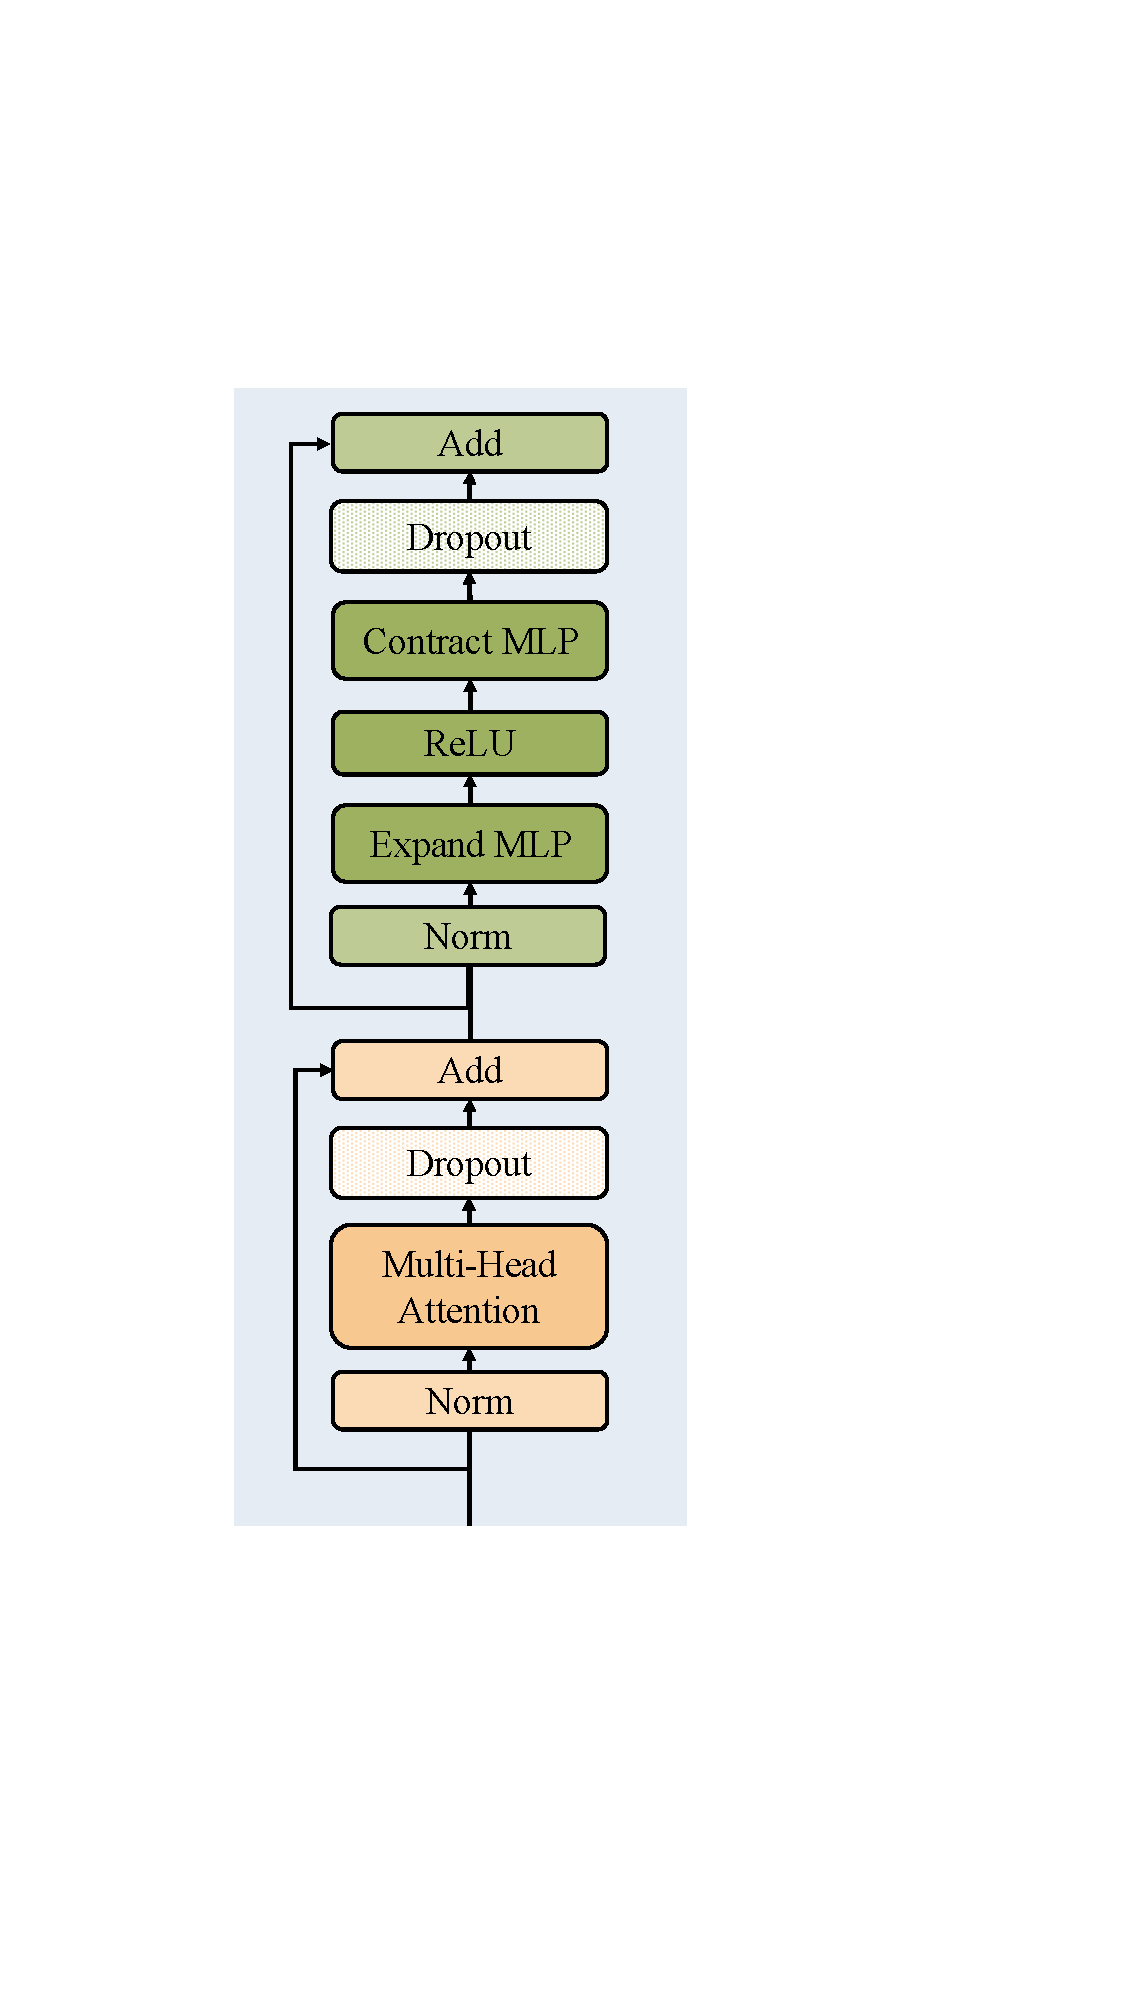
\includegraphics[width=0.18\textwidth]{figure/GPT_Blog_Diagram.pdf}
%   \end{center}
%   \vspace{-4mm}
%     \label{fig:arch}
%     \caption{OPT Architecture}
%       \vspace{-2mm}
% \end{wrapfigure}

\noindent \textbf{Quantization, pruning, distillation for LLM inference.} Various system relaxations have been studied for decades for model inference in machine learning. For example, quantization~\cite{han2015deep, jacob2018quantization,nagel2019data,zhao2019improving}, pruning~\cite{molchanov2016pruning,liu2018rethinking,he2019filter,hoefler2021sparsity}, and distillation~\cite{hinton2015distilling,cho2019efficacy,tang2019distilling,touvron2021training}  have been applied to speed up the inference of the machine learning model. Active research has recently attempted to apply such techniques in LLM inference. For example, zeroQuant~\cite{yao2022zeroquant} and nuQmm~\cite{park2022nuqmm} implement customized CUDA kernels to support tenor-wise or group-wise quantization for LLM inference; LLM.int8 \cite{dettmers2022llm} adopts a mixed \texttt{INT8/FP16} computation to diminish the influence of activation outliers; SmoothQuant~\cite{xiao2022smoothquant} enables efficient 8-bit weight and activation for LLM inference; GPTQ~\cite{frantar2022gptq} adopts a one-shot weight quantization method based on approximate second-order information for accuracy and efficiency; SparseGPT~\cite{frantar2023massive} introduces an approximate sparse regression solver to enable the sparsity in LLM inference; \cite{bansal2022rethinking} has reported that a small set of attention heads can perform primitive induction operations associated with in-context learning, and use this property to prune LLM for acceleration. 

%subsection{Various versions of the efficient large language model.}



%\subsection{Quantization, pruning, distillation}
%old techniques from 1990. no matter image or language


\noindent \textbf{Residual connections in neural networks.} Residual connection shows great advantages for neural network generalization, it provides additional paths for activations to reach the latter parts of the neural network by skipping some layers~\cite{he2016deep}. The advancement of residual connections can be viewed as ensembles of multiple shallow neural networks~\cite{veit2016residual}. Plenty of active research has discussed the effectiveness of residual connections~\cite{balduzzi2017shattered,bello2021revisiting,allen2019can,frei2019algorithm}. However, as far as we know, there is no former work that leverages the property of residual connections to improve the efficiency of LLM inference.  




\section{Additional Observation on Slowly Changing Observation}
\label{sec:appendix-obs}

First, we present more plots on the cosine similarity between representations. Figure~\ref{appendix:observation_changing} plots the cosine similarity between activation across layers on OPT family. It is evident that similarity is high for the larger models.

There are two residual connections inside a transformer layer, one around the attention block, and the other one around the MLP block. The residual connection can be written as $X + F(X)$, where $F$ is either the Multi-Head Attention or two MLP Layer. Figure~\ref{appendix:residual} plots the cosine similarity between $X$ and $X + F(X)$, which is close to 1.0, and the cosine similarity between $X$ and $F(X)$, which is close to 0.0. This happens because $\|X\|$ is significantly greater than $\|F(X)\|$, shown in the purple. In the first layer, $\|F(X)\|$ is larger, which explains the low cosine similarity. The magnitude of the $L2$ norm is different across models, however, we observe a similar trend with models of different sizes. There exists a normalization layer before $F(X)$ and the layer normalization scale $\|X\|$ to a consistent magnitude across layers (e.g. 85 for OPT-30B, 110 for OPT175B), but not necessarily scale down $\|X\|$.

\begin{figure}[t]
  \centering
     \subfigure[OPT-1.3B]{
    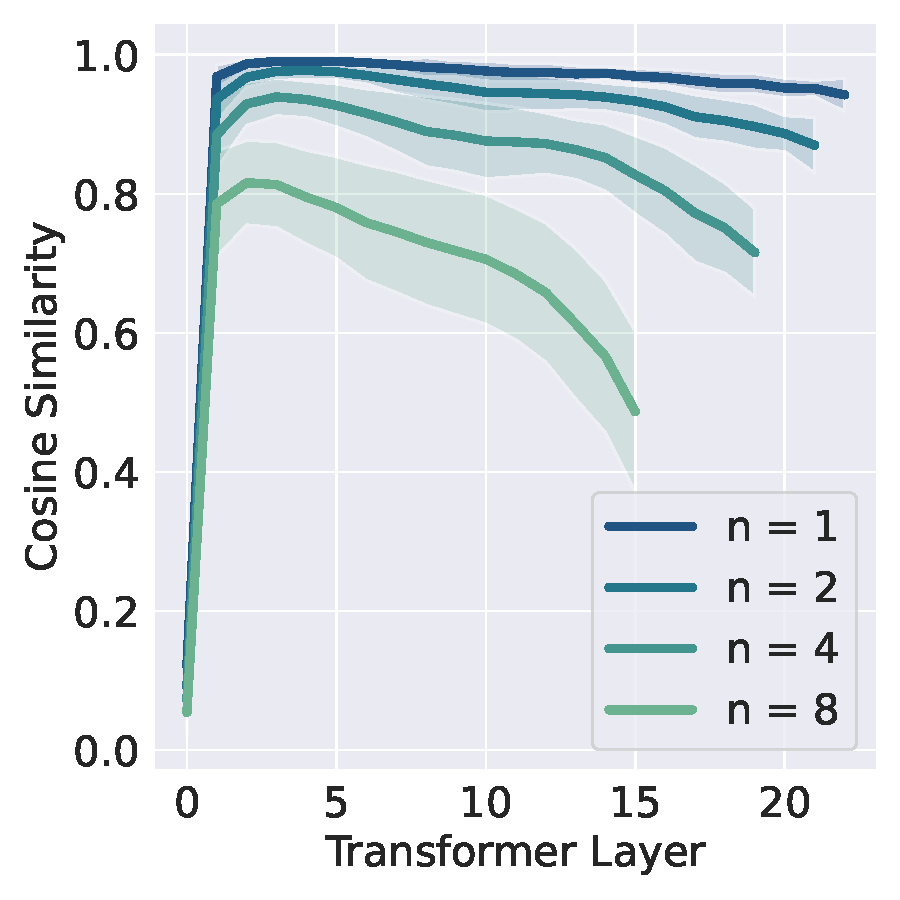
\includegraphics[width=0.30\textwidth]{figure/observation/1.3b_between_layer_cos.pdf}
    }
   \subfigure[OPT-6.7B]{
    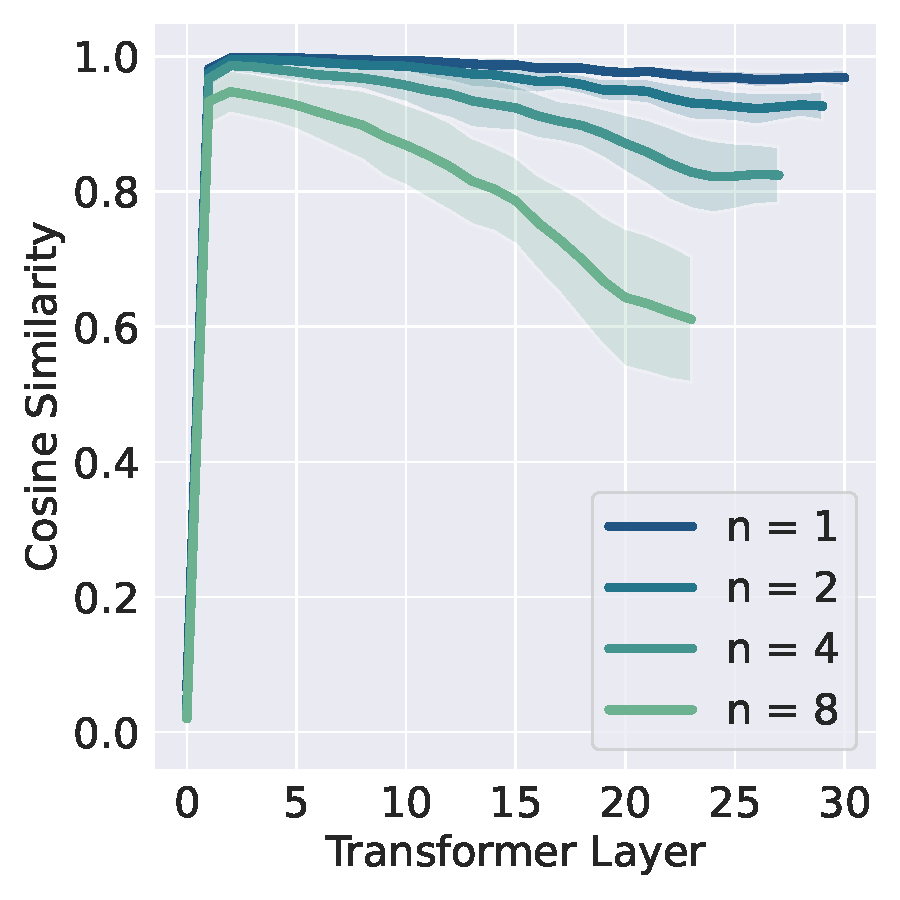
\includegraphics[width=0.30\textwidth]{figure/observation/6.7b_between_layer_cos.pdf}
    }
 \subfigure[OPT-13B]{
    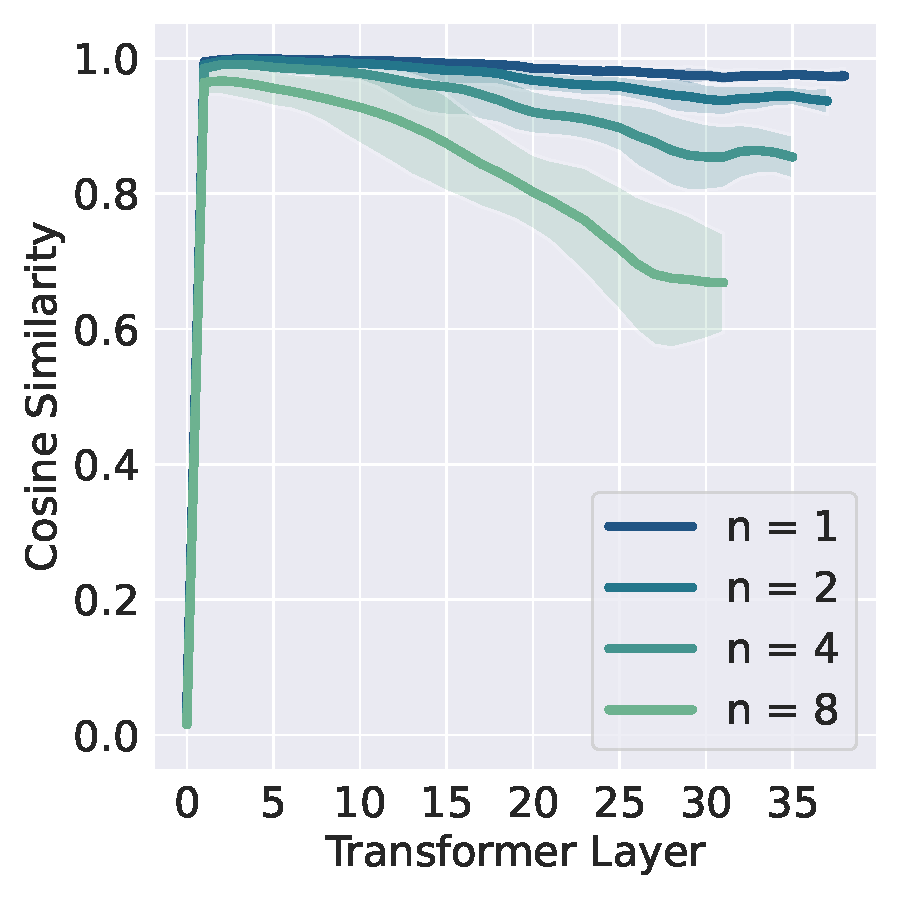
\includegraphics[width=0.30\textwidth]{figure/observation/13b_between_layer_cos.pdf}
    }
  \subfigure[OPT-30B]{
    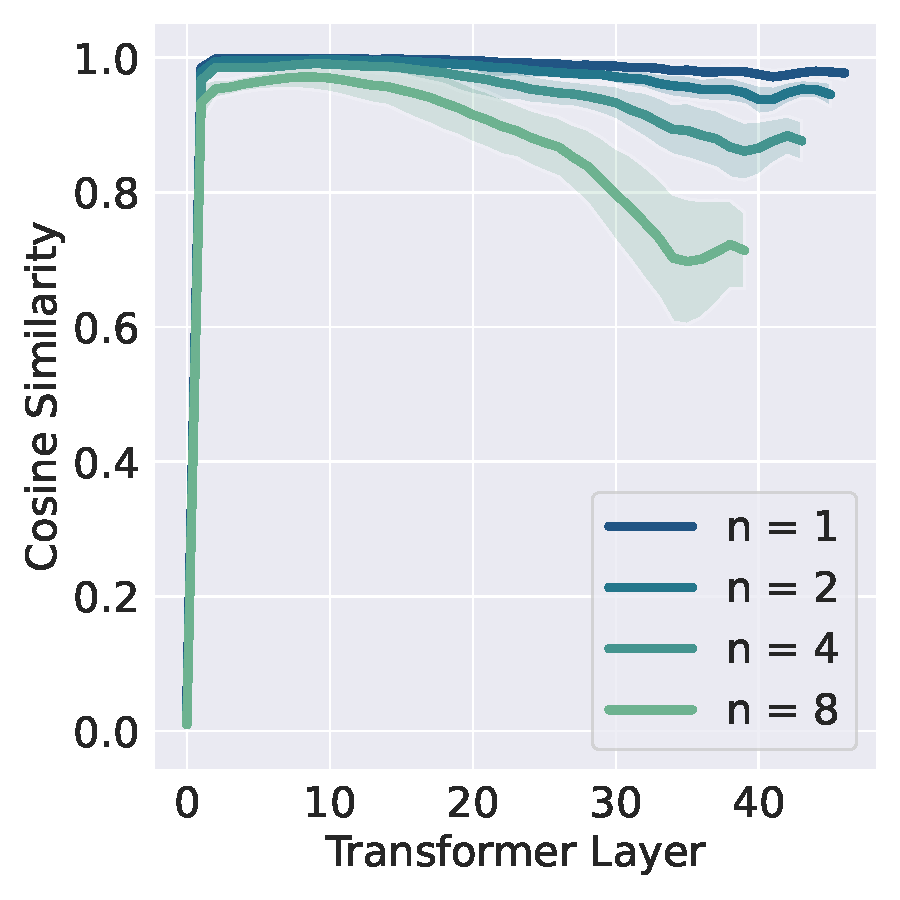
\includegraphics[width=0.30\textwidth]{figure/observation/30b_between_layer_cos.pdf}
  } 
    \subfigure[OPT-66B]{
    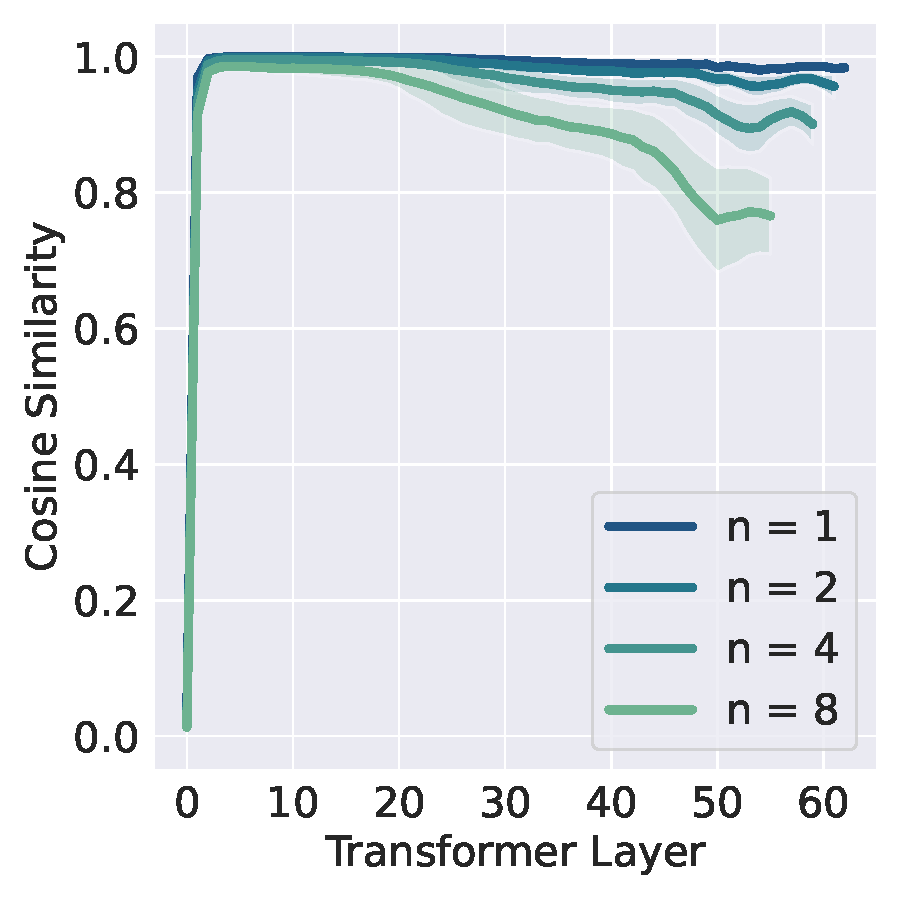
\includegraphics[width=0.30\textwidth]{figure/observation/66b_between_layer_cos.pdf}
  } 
    \subfigure[OPT-175B]{
    \hspace{1mm}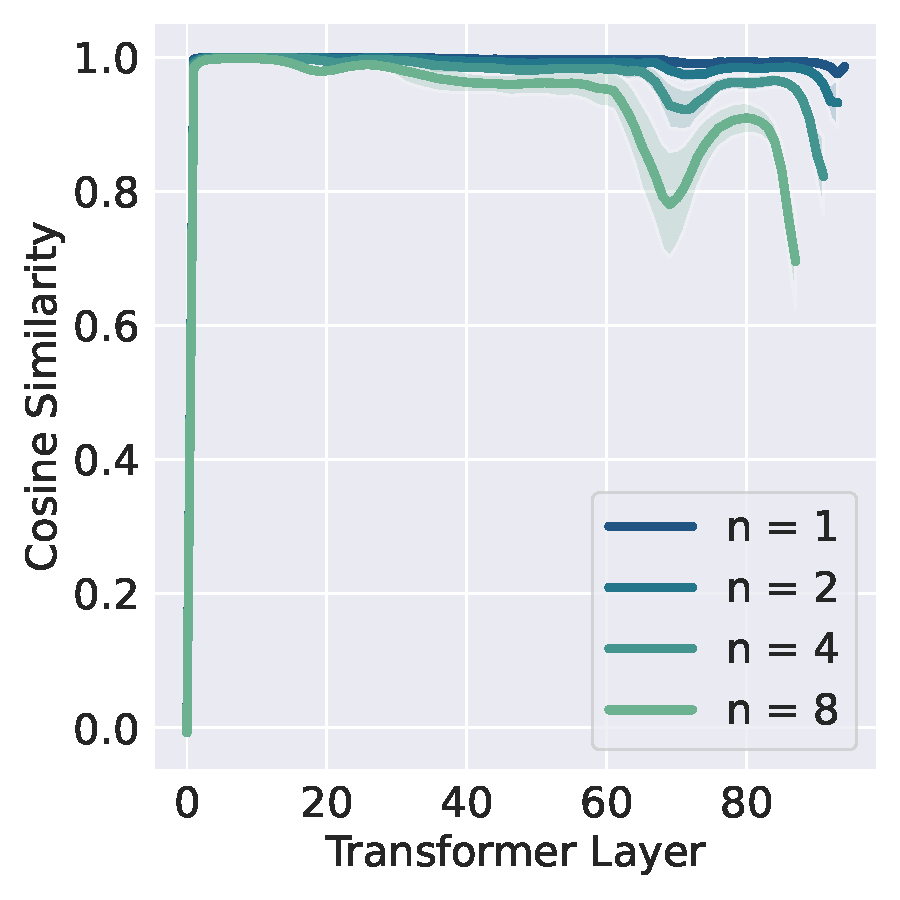
\includegraphics[width=0.30\textwidth]{figure/observation/175b_between_layer_cos.pdf}
  } 
  
  \caption{ Cosine similarity between layer $l$ and layer $l+1$ for various model.}
  \label{appendix:observation_changing} 
\end{figure}

\begin{figure}[t]
  \centering 
    \subfigure[OPT-1.3b]{
    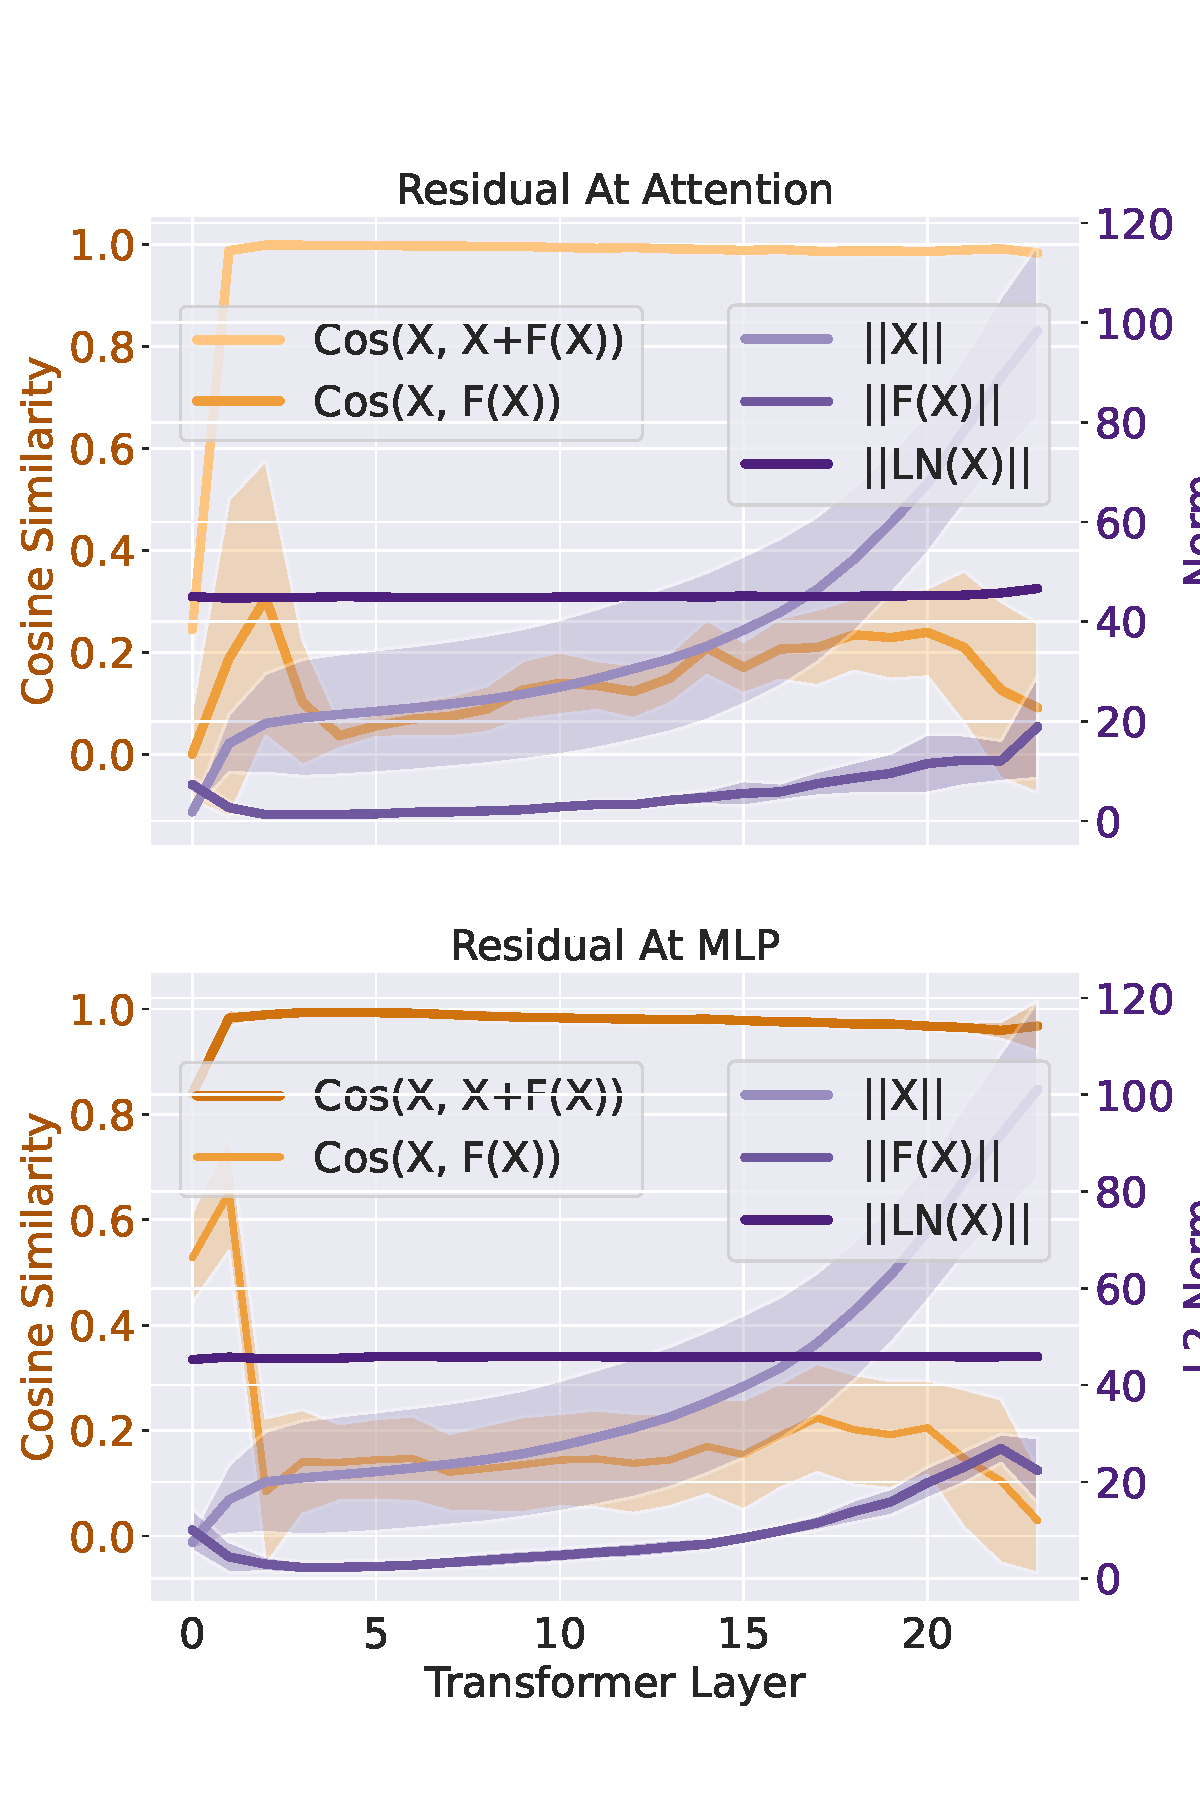
\includegraphics[width=0.30\textwidth]{figure/observation/1.3b_residual_before_after.pdf}
    }
   \subfigure[OPT-6.7b]{
    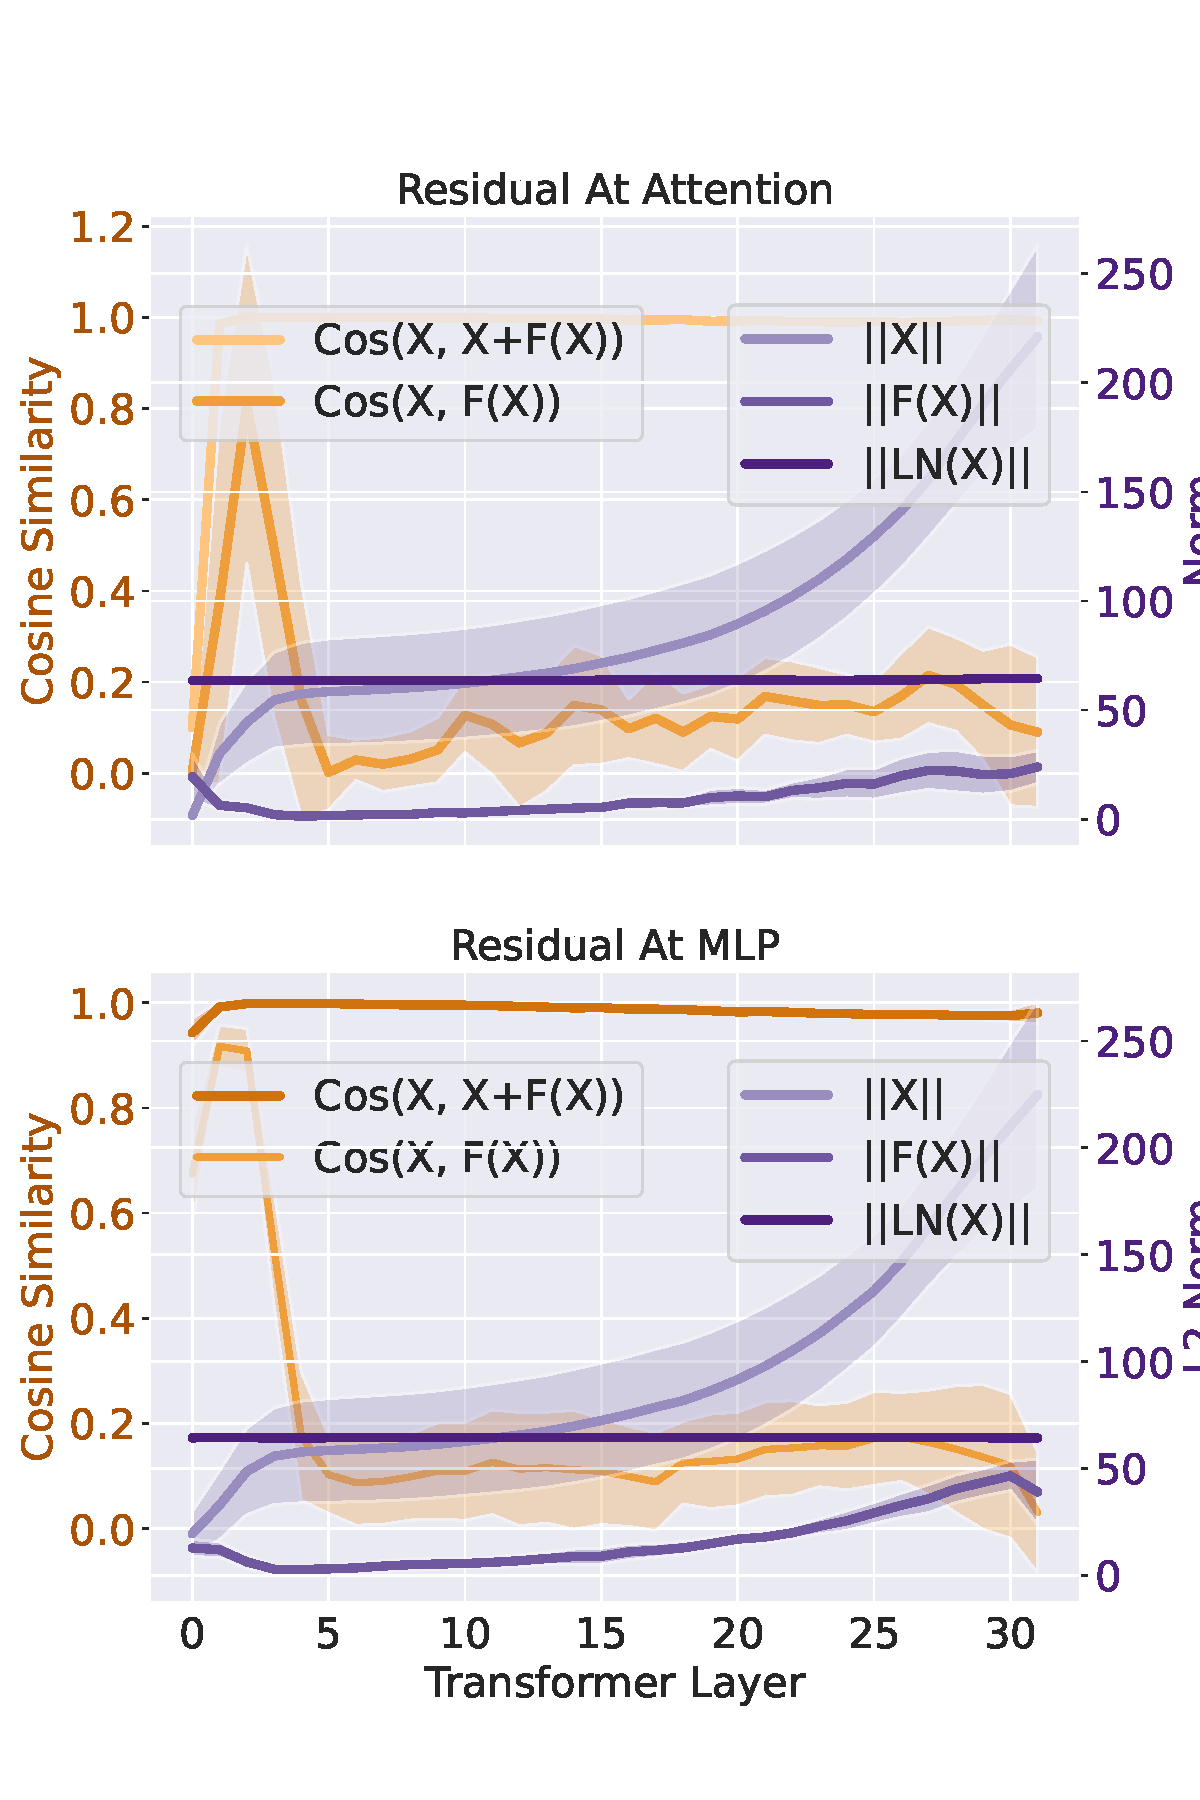
\includegraphics[width=0.30\textwidth]{figure/observation/6.7b_residual_before_after.pdf}
    }
 \subfigure[OPT-13B]{
    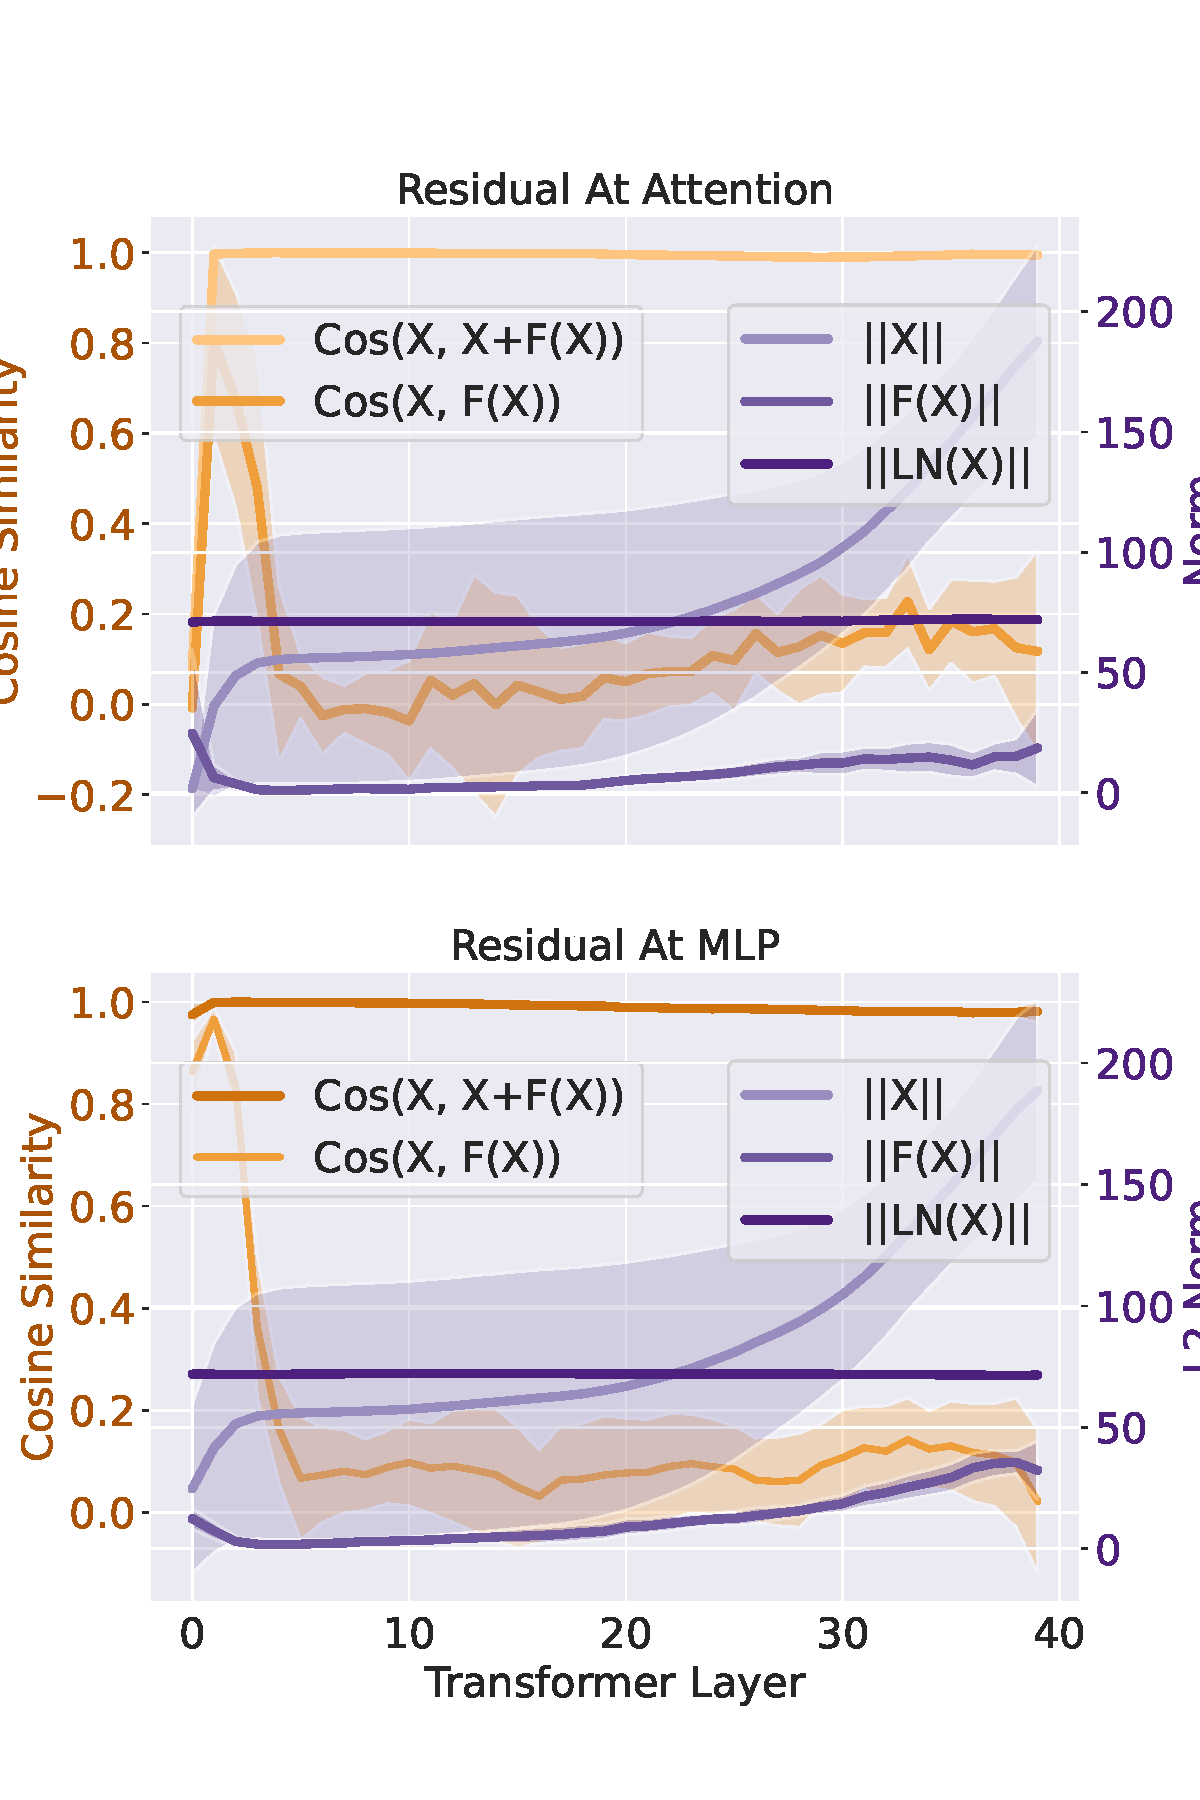
\includegraphics[width=0.30\textwidth]{figure/observation/13b_residual_before_after.pdf}
    }
  \subfigure[OPT-30B]{
    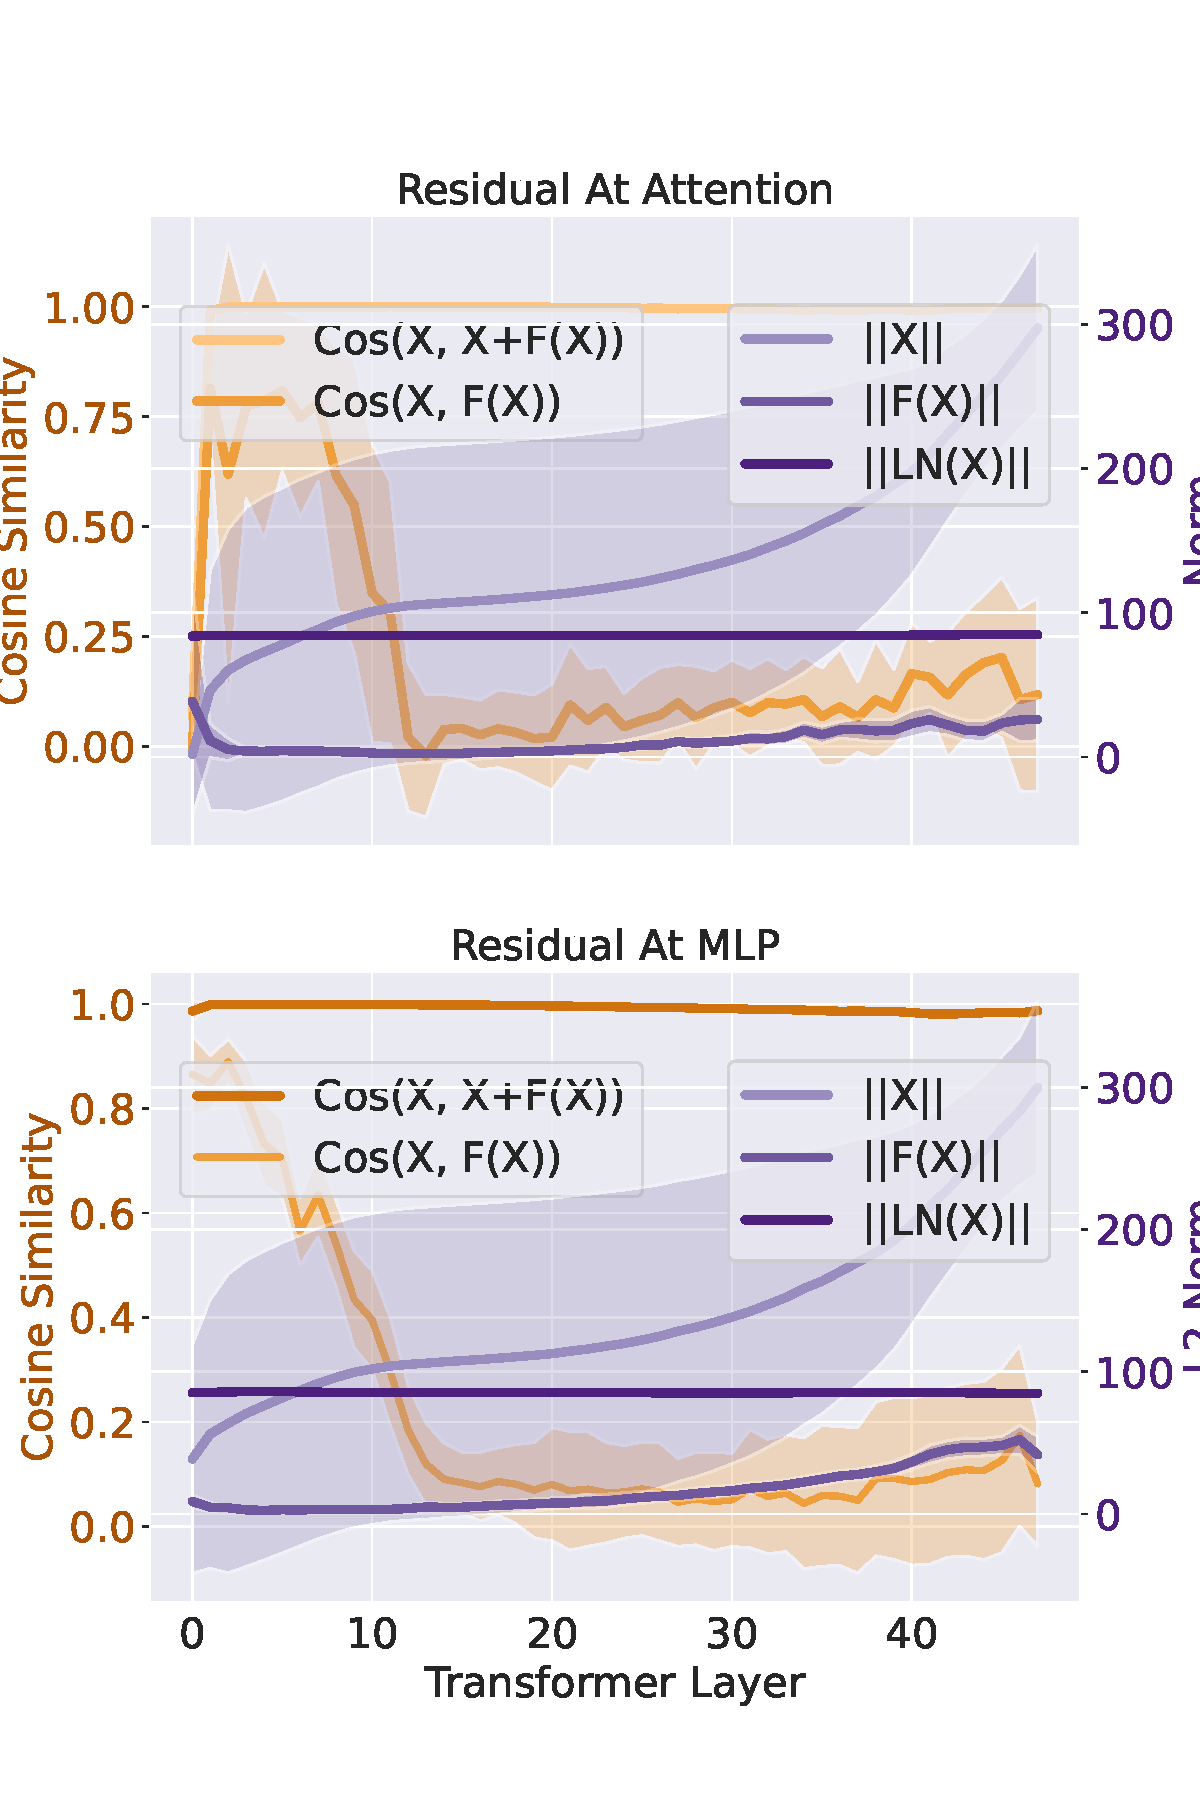
\includegraphics[width=0.30\textwidth]{figure/observation/30b_residual_before_after.pdf}
  } 
    \subfigure[OPT-66B]{
    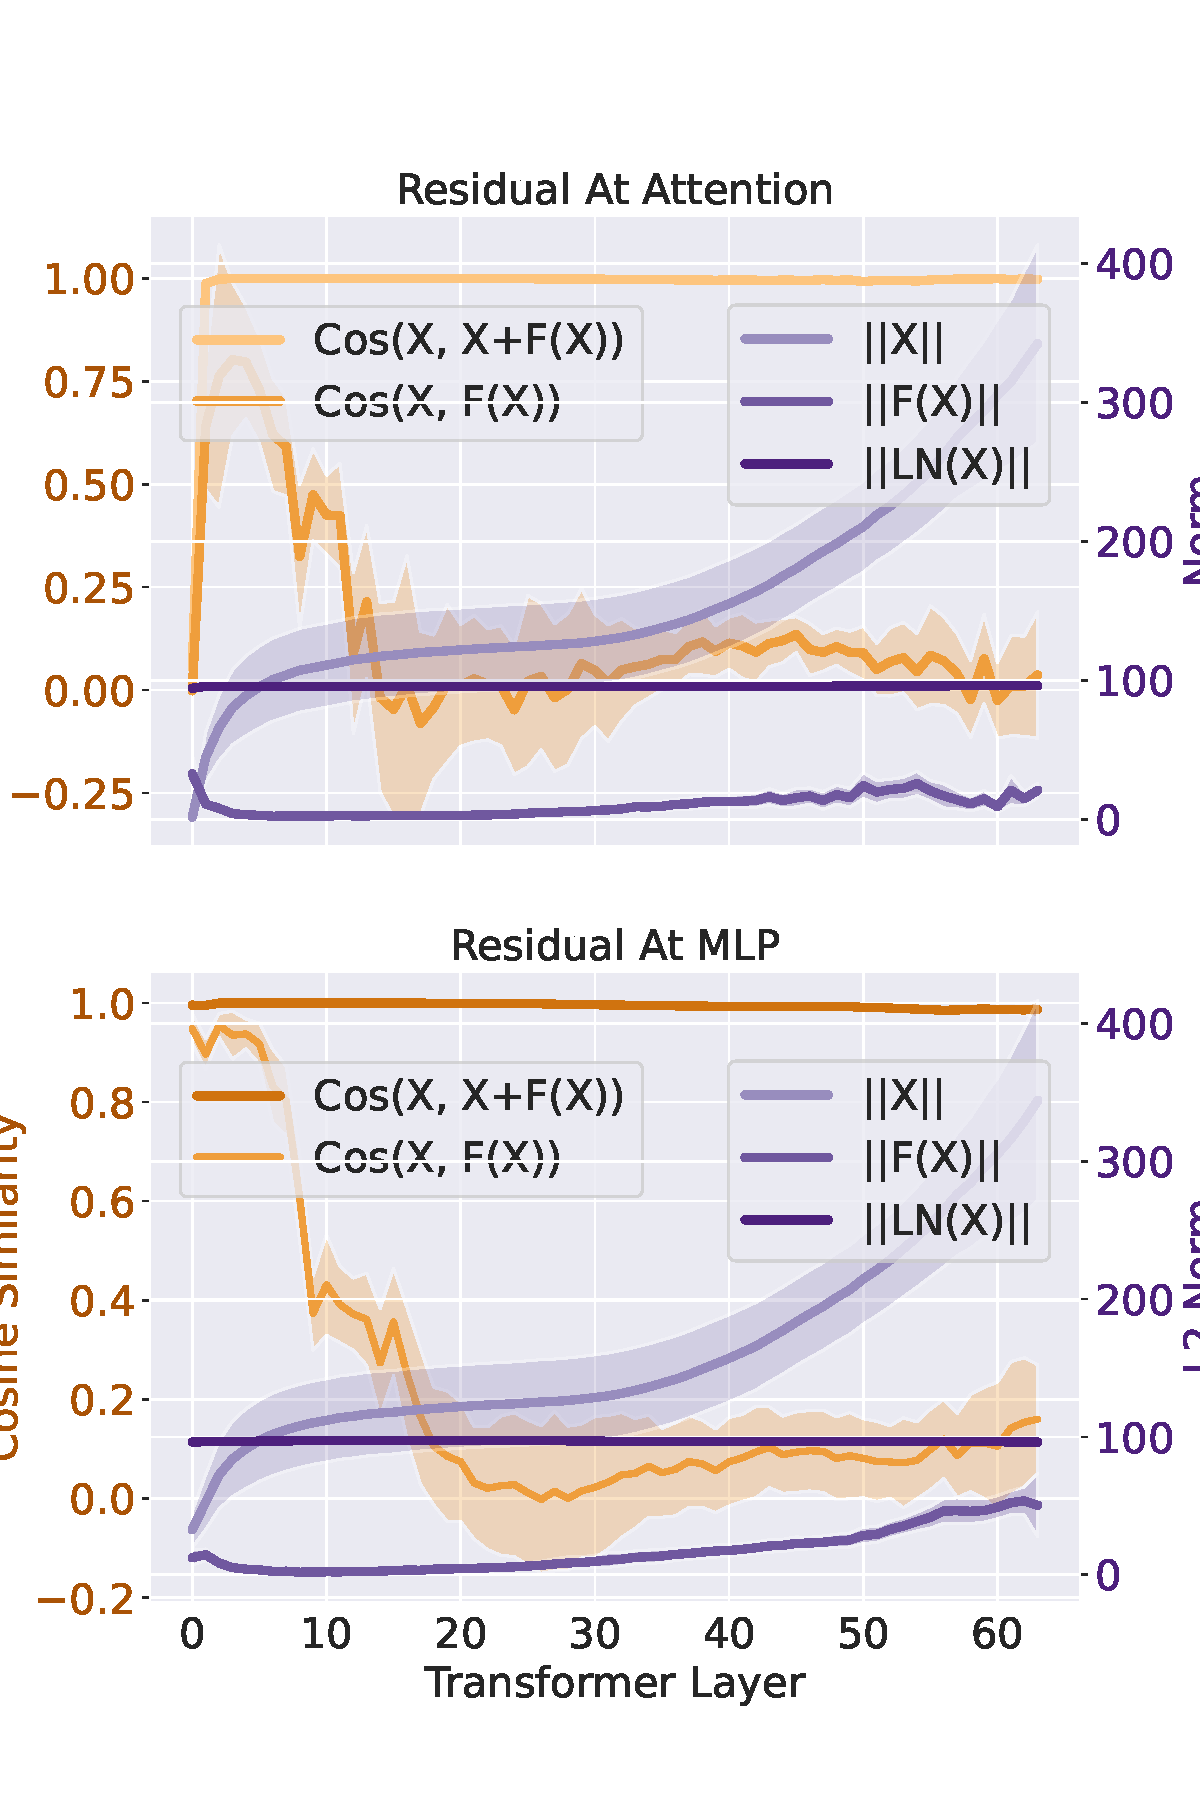
\includegraphics[width=0.30\textwidth]{figure/observation/66b_residual_before_after.pdf}
  } 
    \subfigure[OPT-175B]{
    \hspace{1mm}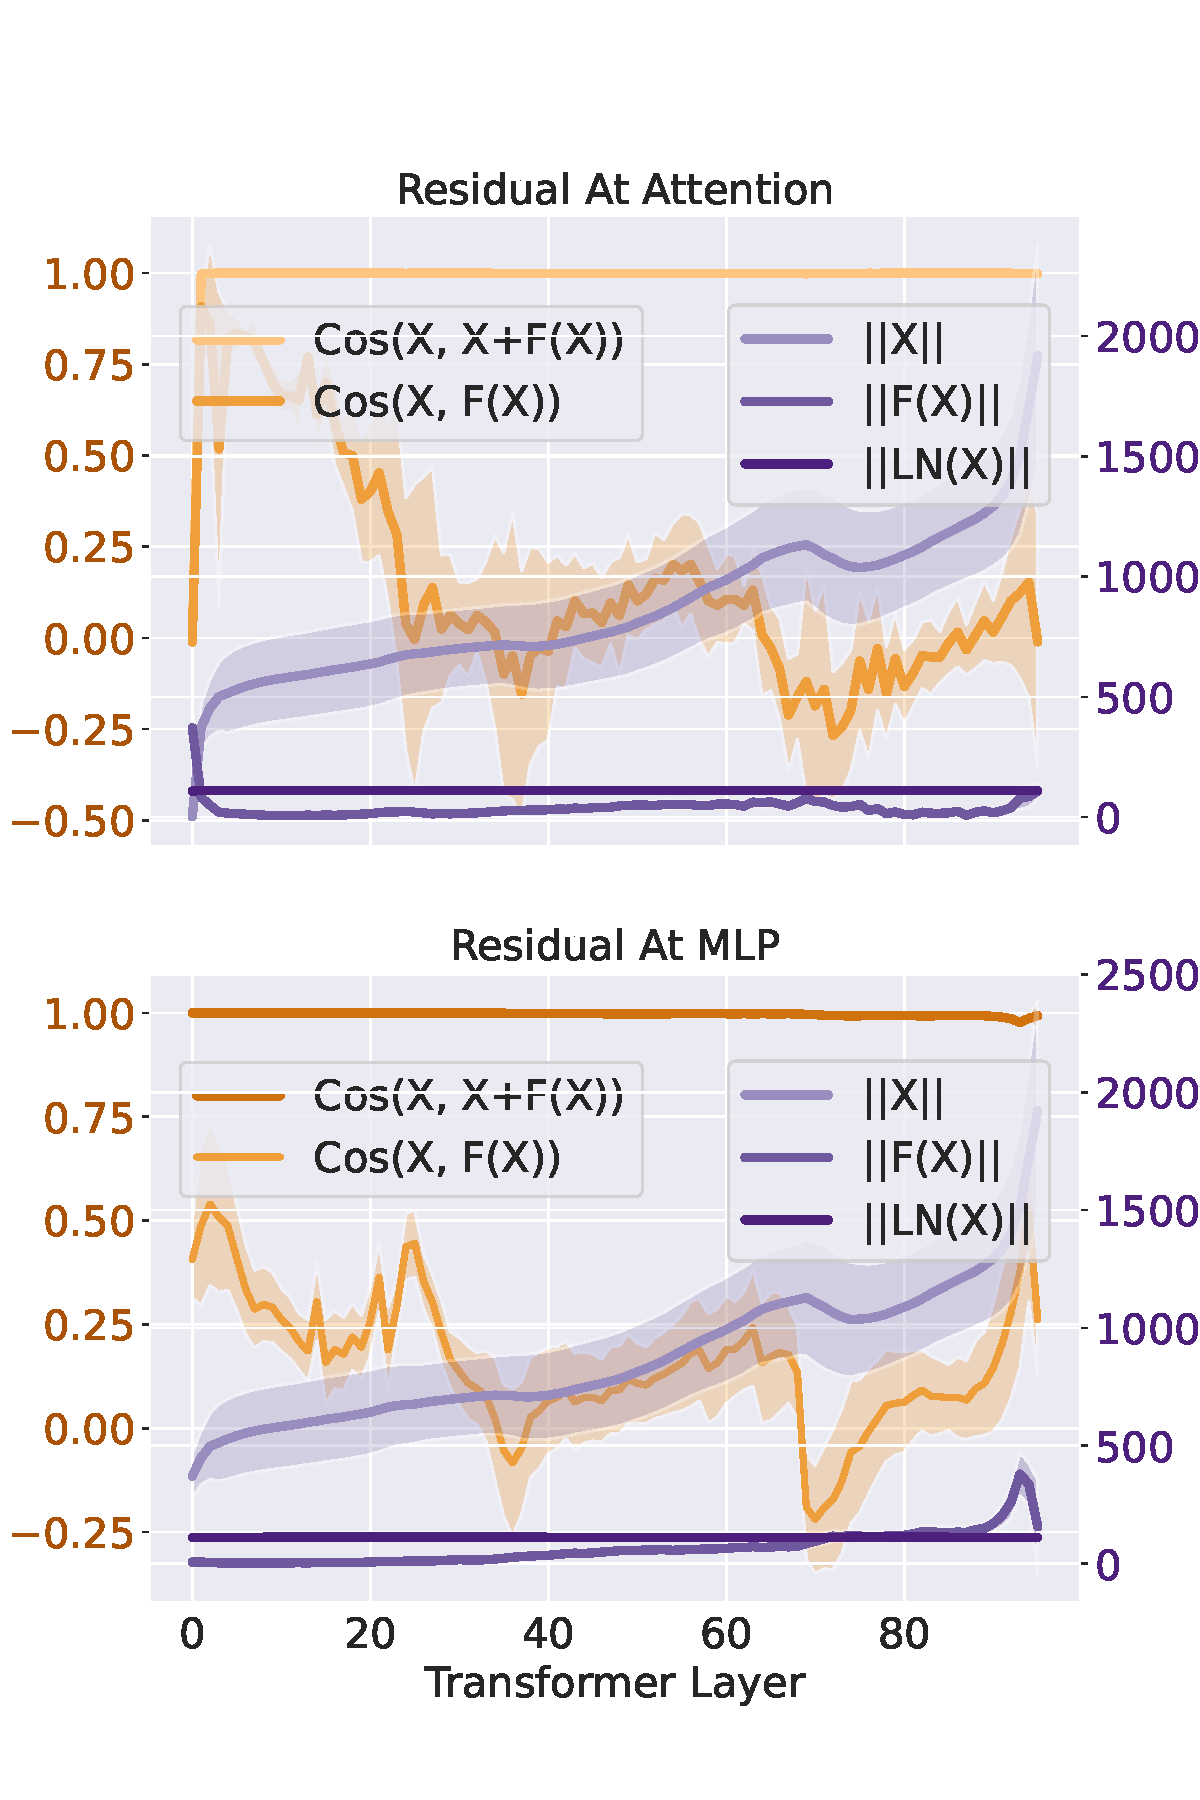
\includegraphics[width=0.30\textwidth]{figure/observation/175b_residual_before_after.pdf}
  } 
  \caption{ Cosine similarity between $X$ and $F(X)$, and the cosine similarity between $X$ and $X'$ in orange color. $L2$ norm of $X$ and $F(X)$ and $X$ after layer normalization in purple on the right. Except on the first layer, $\|X\|$ is significantly higher than $\|F(X)\|$. $\|F(X)\|$ is higher at the first layer, which corresponds to the low cosine similarity at the first layer.}
  \label{appendix:residual} 
\end{figure}

\section{Additional Experiment Detail}
\label{sec:appendix-exp}
\subsection{Large Batch Size}
To help understand where the speed-up comes from when batch size is greater than 1, we present the Union Contextual Sparsity (fraction of neurons/heads that are not used by any of the inputs in the batch) of different batches sizes for MLP and Attention blocks, respectively, in Figure~\ref{appendix:exp_sparsity_batch}. Union Contextual Sparsity is calculated as 1.0 - the union of activated MLP neurons or Attention heads in the batch / total neurons or heads. The union operation is essential to realize a fast sparse GEMM. 

Surprisingly the number of MLP neurons/Attention heads that \name{} activated does not grow linearly with the batch size. This suggests a power law distribution rather than a uniform distribution of parameter access from all input examples. Further, a larger batch size can easily lead to out-of-memory for long sequence settings due to the limited GPU memory, the giant large model size, and the stored KV cache. For example, the total GPU memory of 8 80GB A100 is 640GB. Model parameters are around 350GB for OPT175B. The KV cache for a batch size 32 with a sequence longer than 1920 tokens has already filled up the GPU memory. 

\begin{figure}[h]
  \centering
     \subfigure[MLP]{
    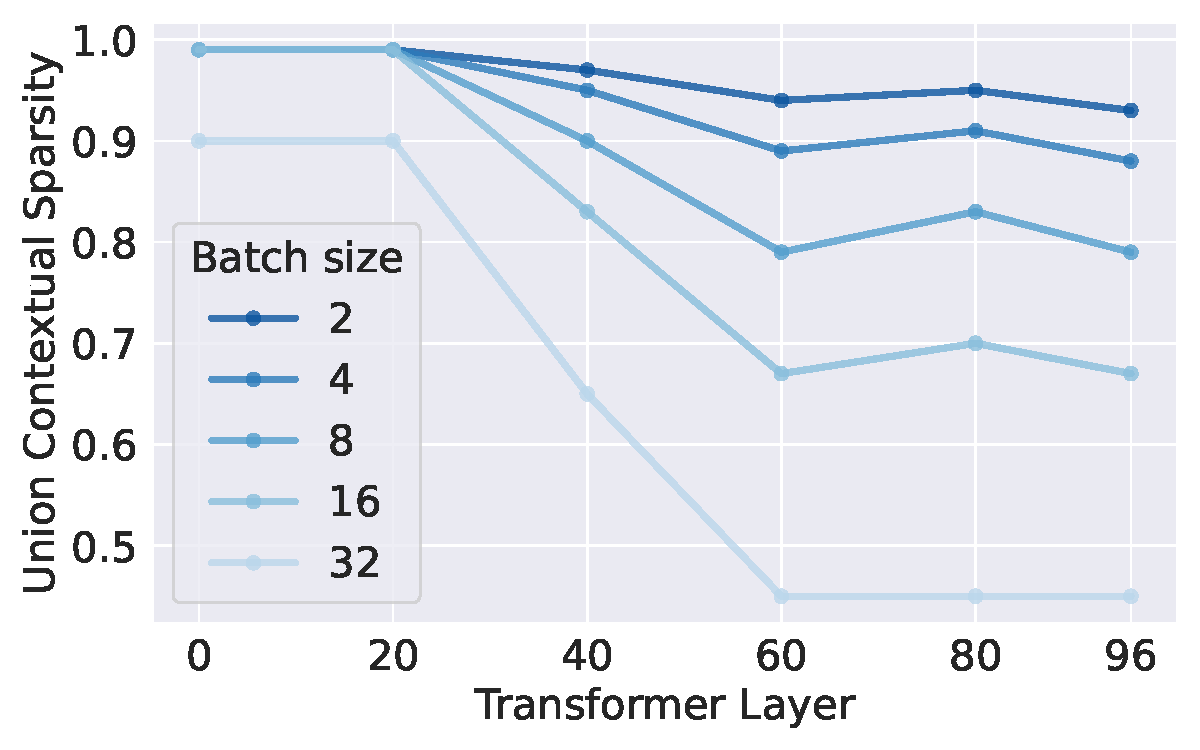
\includegraphics[width=0.40\textwidth]{figure/experiment/batch_sparsity_mlp.pdf}
    }
   \subfigure[Attention]{
    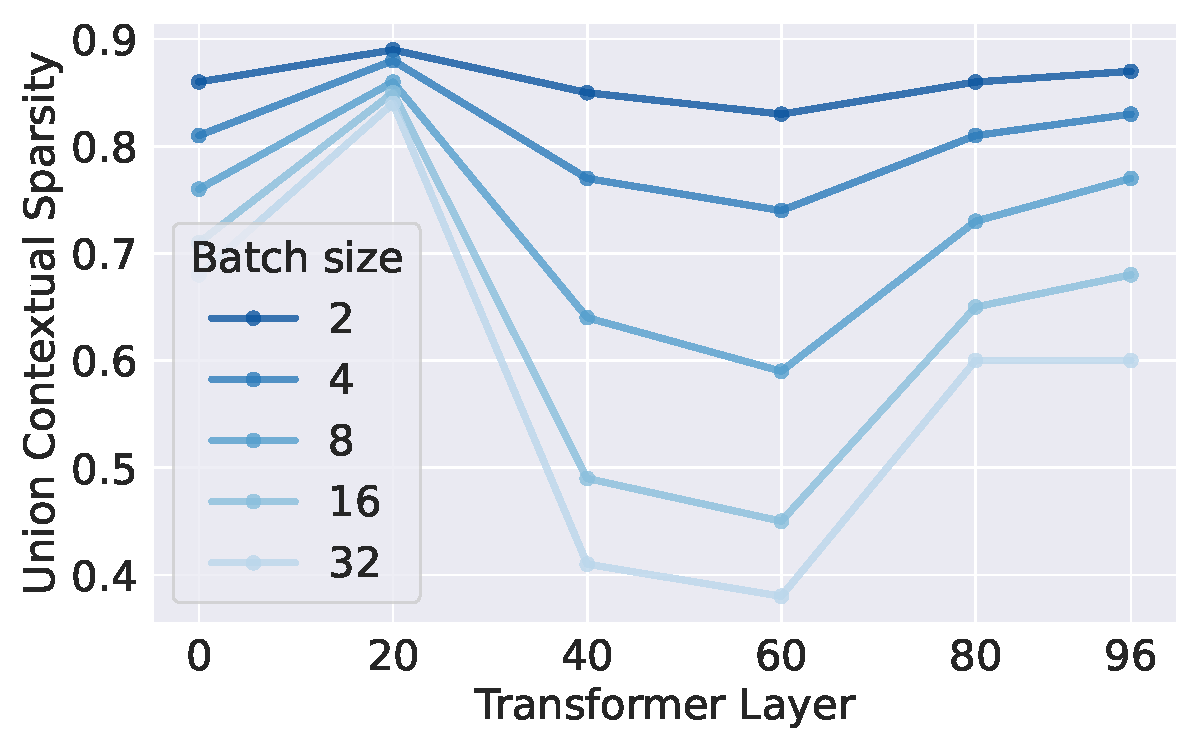
\includegraphics[width=0.40\textwidth]{figure/experiment/batch_sparsity_attention.pdf}
    }
  \caption{Union contextual sparsity with larger batch size.}
  \label{appendix:exp_sparsity_batch} 
\end{figure}
\subsection{Near Neighbor classifier}
In the \name{} framework, any near-neighbor search method under the inner product metric would be sufficient to predict a sparsity pattern. "Training predictor" is to reduce the cost of on-the-fly prediction, rather than training the model itself.

For example, in our exploration stage mentioned in Section 4.1, we adopt HNSW, a state-of-art near-neighbor search method, to predict MLP sparse pattern, and we can see from the following table there is no drop in the perplexity at 90 \% sparsity ratio. However, due to the high dimensionality of embedding and HNSW’s reliance on CPU, the time HNSW took to identify the sparsity pattern is 10ms, which is longer than the MLP computation.

\begin{table}[h]
\centering
\begin{tabular}{ccc}
\hline
          & OPT-1.3B & OPT-1.3B + HNSW \\
\hline
Hellaswag & 0.4154   & 0.4314          \\
C4        & 14.2     & 14.4           \\
\hline
\end{tabular}
\end{table}
In our paper, we choose a neural network classifier as our near neighbor search method to take advantage of the fast matrix multiplication on GPU. And training such classifiers to predict sparsity patterns is not only cheaper in terms of training cost but also inherently different from the method concept.
\subsection{Future Possibility: Skipping Layer}
\label{sec:exp_skip_layer}


\label{sec:block_parallel}
Deja Vu currently sparsifies from the perspective of model width. Here, we explore the possibility of sparsification from model depth. 
As observed in \cref{sec:obs}, we show that the activation of large language models changes slowly across blocks. This property can be leveraged to increase the efficiency of a trained model by parallelizing, reordering, or skipping certain intermediate sub-blocks without significantly impacting the overall accuracy. 
\begin{table}[t]
\scriptsize
\centering
\caption{ Sparsify from the Depth: Skipping or parallel entire transformer blocks may not lead to catastrophic drop in accuracy at test time.}
\resizebox{0.6\linewidth}{!}{
\centering
\Huge
\begingroup
\setlength{\tabcolsep}{10pt}
\renewcommand{\arraystretch}{1.3}
\begin{tabular}{l||cccccc}
\specialrule{.15em}{.05em}{.05em}
 Model & COPA & Hellaswag & Lambada & OpenBookQA & PIQA  & Winogrande	\\
\cline{1-7}
 OPT-175B        
            & 0.8600 & 0.7814  & 0.7584 & 0.4460 & 0.8096 &  0.7261 \\
 \, - Parallel 2  
            & 0.8300 & 0.7737  & 0.7762 & 0.4520 & 0.8030 & 0.7096 \\
 \, - Parallel 4  
            & 0.5200 & 0.2519  & 0      & 0.2720 & 0.5092 & 0.4870 \\
 \, - Skip 2/8  
            & 0.8000 & 0.7112  & 0.6387 & 0.4220 & 0.7840 & 0.6630 \\
 \, - Skip 2/4 
            & 0.6900 & 0.4409  & 0.0240 & 0.3400 & 0.6882 & 0.5383 \\
\cline{1-7}
Bloom         
            & 0.8000  & 0.7460  & 0.6771 & 0.4480 & 0.7949 & 0.7040  \\
\, - Parallel 2   
            & 0.8100  & 0.7404  & 0.6992 & 0.4360 & 0.7813 & 0.7048 \\
\, - Parallel 4
            & 0.6200  & 0.3176  & 0.1325 & 0.2720 & 0.5593 & 0.5217 \\
 \, - Skip 2/8  
            & 0.7900 & 0.6829  & 0.5936 & 0.4120 & 0.7699 & 0.6614 \\
 \, - Skip 2/4 
            & 0.6600 & 0.5538  & 0.3023 & 0.3580 & 0.7046 & 0.5549 \\
\specialrule{.15em}{.05em}{.05em}
\end{tabular}
\endgroup
}
\end{table}
\begin{table}[ht]
\scriptsize
\centering
\resizebox{0.3\linewidth}{!}{
\centering
\Huge
\begingroup
\setlength{\tabcolsep}{10pt}
\renewcommand{\arraystretch}{1.3}
    \begin{tabular}{lrr}
    \toprule
    Setting                 & Wiki(ppl) & C4(ppl) \\
    \midrule
    Baseline                &  11.57    &   10.17    \\
    % Parallelize  2 blocks   &           &          \\
    % Parallelize  4 blocks   &   nan     &    nan    \\
    Skip every 2 layers      &  21.16    &   16.58   \\
    Skip every 4 layers      &  13.45    &   11.37  \\
    % Skip every 8 layers      &  12.37    &           \\
    \bottomrule
    \end{tabular}
\endgroup
}
\label{table:corruption}
\end{table}


Improving the inference efficiency of Transformer models is a challenging task due to their sequential execution of Transformer layers.
Each sub-block depends on the output of the previous one, leading to low hardware efficiency, particularly during the token generation phase where each forward pass is computed for only one token.
% To address this issue, various solutions have been proposed such as pipeline parallelism \cite{} and tensor parallelism \cite{}.
However, the sequential execution of blocks and sub-blocks yields computation bubbles, and the latter involves a large amount of communication overhead. 
Here, we present an interesting observation that can potentially alleviate these challenges. We found that the activation of the model changes slowly across blocks. Specifically, the cosine similarity of activations between adjacent blocks is often above 0.99.
This suggests that the blocks might take the previous activation as input -- parallelize or reorder the blocks -- without significantly affecting the output.
Slowly changing activations suggest that it may be possible to parallelize, reorder, or even skip blocks while maintaining a similar output.
Some existing models, such as GPT-J~\citep{gpt-j}, GPT-NeoX~\citep{gpt-neox-20b}, and PaLM~\citep{chowdhery2022palm} already placed the Attention block and MLP block in parallel in training to facilitate parallel computation and reduce the communication overhead. 

Here we investigate the possibility at inference time. And surprisingly, we found parallelizing those blocks for models that are trained in a sequence manner will not hurt the performance of downstream tasks significantly. And surprisingly, we found parallelizing those blocks for models that are trained in a sequence manner will not hurt the performance of downstream tasks significantly. Table\ref{table:corruption} presents some preliminary results of OPT-175B and Bloom

Given the activation $y$ and Transformer layer $l$, we have:
\begin{align*}
    \widetilde{y}_l \leftarrow y_l + \mathsf{MHA}^{l}(y_l) \\
   \widehat{y}_l \leftarrow \widetilde{y}_l + \mathsf{MLP}^{l}(\widetilde{y}_l)
\end{align*}
Parallelizing two blocks refers to placing the Attention and MLP blocks in parallel, i.e.:
\begin{align*}
    \widehat{y}_l \leftarrow y + \mathsf{MHA}^{l}(y_l) + \mathsf{MLP}^{l}(y_l)
\end{align*}
Parallelizing four blocks then parallelize the blocks of two Transformer layers, defined as follows:
\begin{align*}
    \widehat{y}_{l+1} \leftarrow y_l + \mathsf{MHA}^{l}(y_l) + \mathsf{MLP}^{l}(y_l)
    + \mathsf{MHA}^{l+1}(y_l) + \mathsf{MLP}^{l+1}(y_l)
\end{align*}
Skipping layers is straightforward, which drops an entire Transformer layer for every $n$ layers.


We are surprised to find that parallel two layers preserve accuracy on a series of tasks across models. Besides, randomly skipping 25\% layers doesn't lead to catastrophic quality. Our findings suggest from the downstream task perspective, the activation patterns within the model are relatively consistent across different blocks, providing a potential avenue for future research on model compression and optimization.




% \begin{table}[]
%     \centering
%     \begin{tabular}{lrr}
%     \toprule
%     Setting                  & Wiki(ppl) & C4(ppl) \\
%     \midrule
%     Baseline                 &  10.82    &   8.04      \\
%     Parallelize  0.5 block   &  11.47    &   8.04      \\
%     Parallelize  2 blocks    &           &           \\
%     Parallelize  3 blocks    &   nan     &    nan    \\
%     Skip every 2 blocks      &           &           \\
%     Skip every 4 blocks      &           &           \\
% emma    Skip every 8 blocks      &           &           \\
%     \bottomrule
%     \end{tabular}
%     \caption{OPT-175B, Corruption}
%     \label{tab:opt_corruption}
% \end{table}
% \begin{table}[]
%     \centering
%     \begin{tabular}{lrr}
%     \toprule
%     Setting                 & Wiki(ppl) & C4(ppl) \\
%     \midrule
%     Baseline                &  11.57    &   10.17    \\
%     % Parallelize  2 blocks   &           &          \\
%     % Parallelize  4 blocks   &   nan     &    nan    \\
%     Skip every 2 layers      &  21.16    &   16.58   \\
%     Skip every 4 layers      &  13.45    &   11.37  \\
%     % Skip every 8 layers      &  12.37    &           \\
%     \bottomrule
%     \end{tabular}
%     \caption{Sparsify from the Depth}
%     \label{tab:bloom_corruption}
% \end{table}


% \fi



%%% Local Variables:
%%% mode: latex
%%% TeX-master: "main"
%%% End:

\section{Implementation Details}
\label{appendix:method}

Figure~\ref{fig:sparse_computation_diagram} presents a more detailed workflow of \name{}. The left diagram shows how an input $y$ performs the sparse MHA with selected indices ${0, 3}$, predicted by the head predictor. Similarly, the right diagram shows how an input $y$ performs the sparse MLP with selected indices ${0, 2}$, predicted by the neuron predictor of that layer.

\begin{figure}[h]
  \centering
  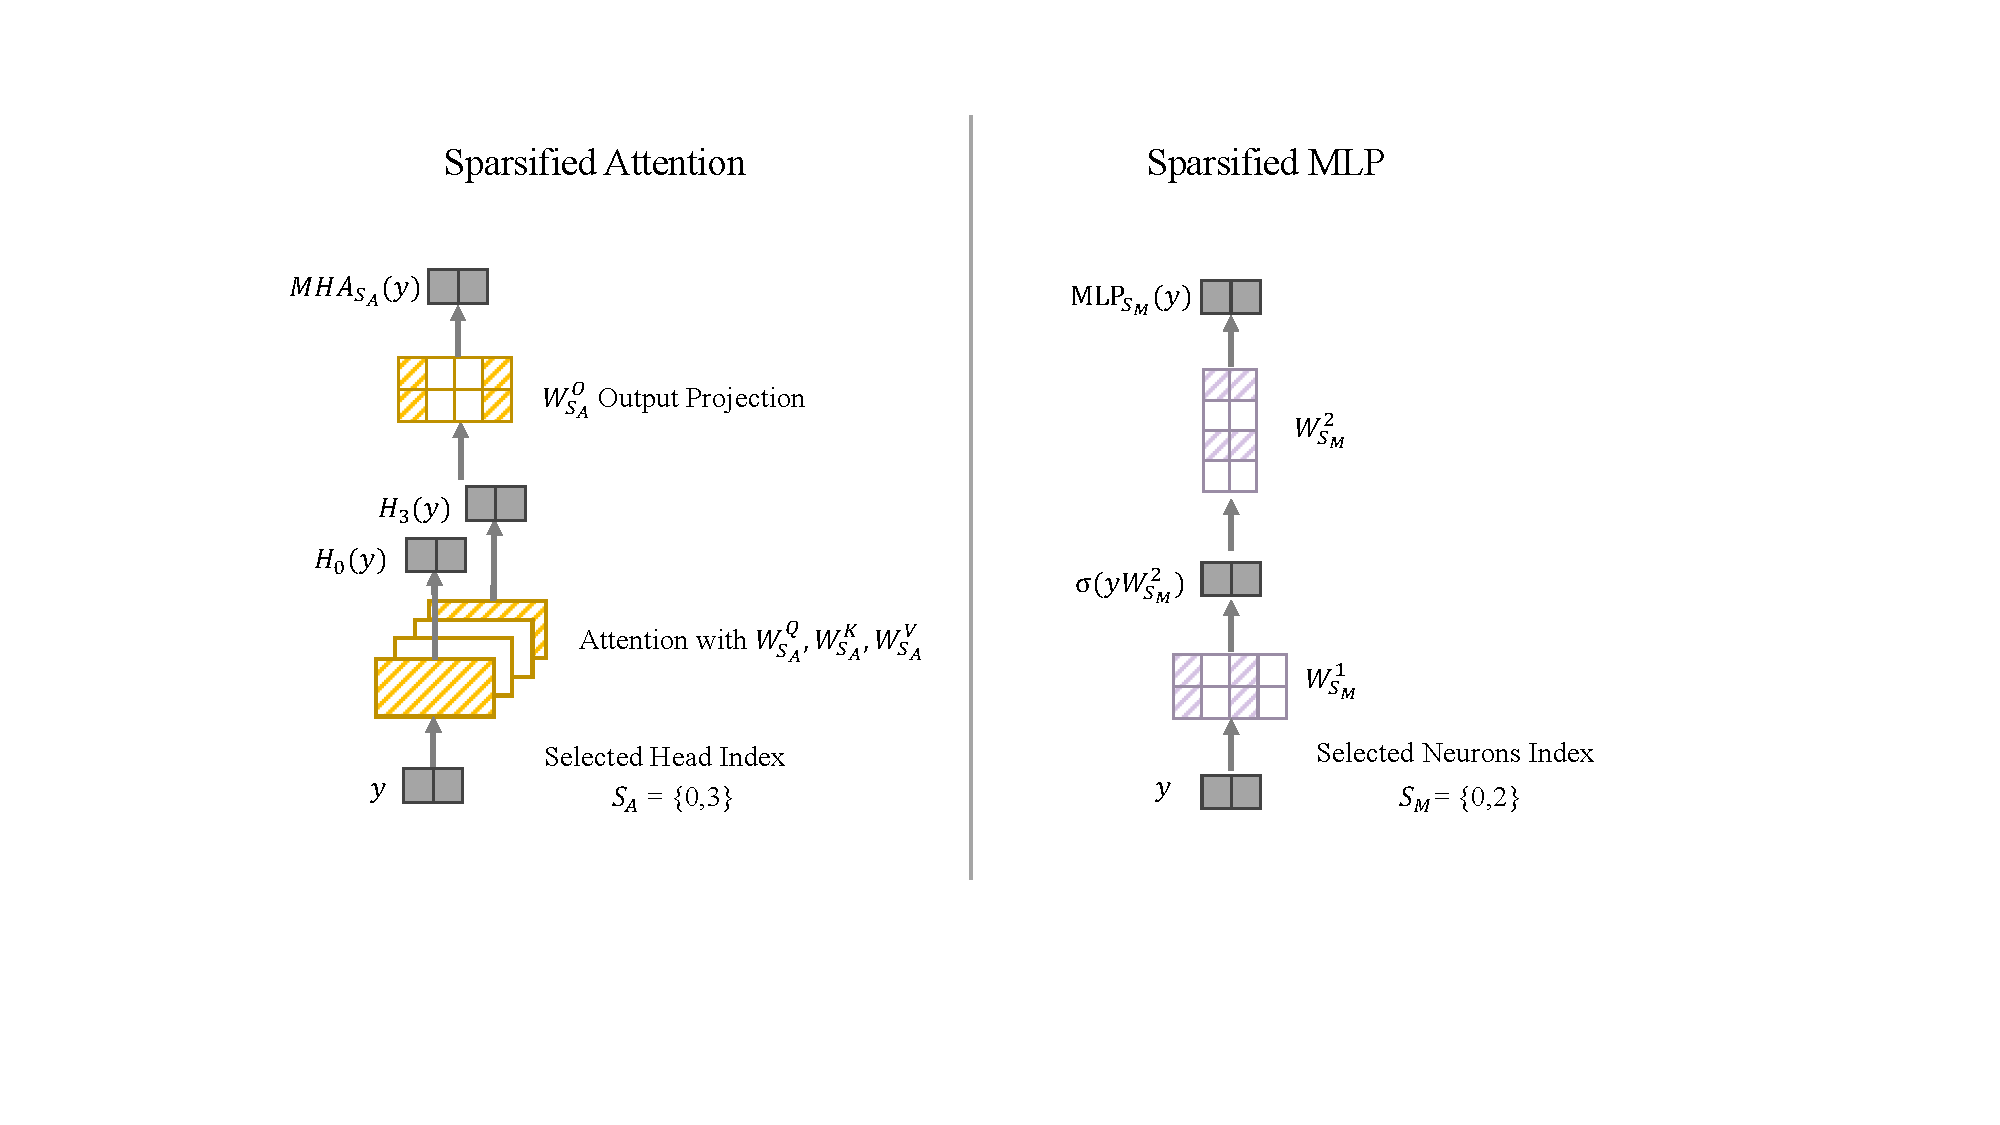
\includegraphics[width=0.8\textwidth]{figure/sparse_computation_diagram.pdf}
  \caption{Detailed diagram on the sparsified computation process of MLP and Attention. Notation refers to Section~\ref{sec:formulation}}
  \label{fig:sparse_computation_diagram}
\end{figure}

Next, we will present a general explanation of two optimizations we used in \name{} implementation. Kernel fusion: A standard implementation of sparse matrix-vector
  multiply (e.g., $Wx$ in PyTorch) that separately indexes a subset of the matrix
  $W[\mathrm{idx}, :]$ before multiplying with input $x$ would incur 3$\times$ the
  amount of memory IOs: one to load a subset of $W$ from GPU memory, one to
  write that subset to a different contiguous region in memory, and one to load
  that (now contiguous) subset in again to multiply with $x$.
  Similarly, to use sparse matrix multiply routines (e.g., cuSparse), we would
  first need to convert $W[\mathrm{idx}, :]$ to sparse format, again incurring
  more memory IOs.
  We instead fuse the indexing and the multiplication step: we load a subset of
  $W[\mathrm{idx}, :]$ to memory, along with $x$, perform the multiply, then
  write down the result.
  This fused implementation (in Triton~\citep{tillet2019triton}) yields up to
  4$\times$ speedup compared to a standard PyTorch implementation (Section~\ref{sec:mlp_attn_benchmarks}). Memory coalescing: the weight matrices are conventionally stored in
  row-major format.
  This allows us to load $W[\mathrm{idx}, :]$ optimally (as the second dimension
  is contiguous in memory).
  However, for cases where we need to load $W[:, \mathrm{idx}]$ (attention
  output projection and the 2nd weight matrix in the MLP) this format
  significantly slows down memory loading, as $\mathrm{idx}$ could contain
  indices pointing to non-contiguous memory.
  A simple solution is to store these matrices in column-major format (i.e.,
  storing $W^\top$ in contiguous row-major format), then use the same fused kernel
  above.
  This transposition is done once when loading the model, and incurs no added
  cost during generation.
\section{Benchmarking Sparse MLP and Sparse Attention}
\label{sec:mlp_attn_benchmarks}

\begin{figure}[h]
  \centering
  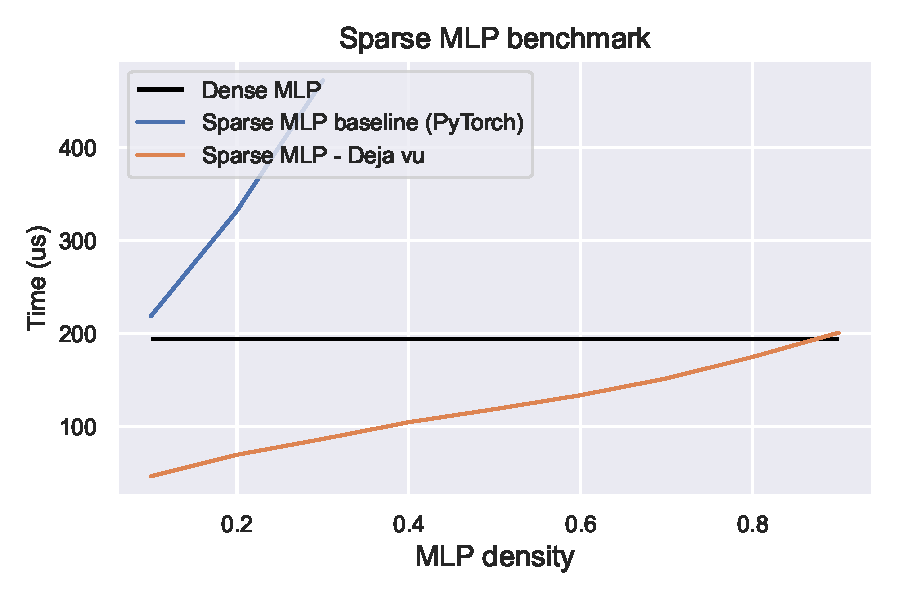
\includegraphics[width=0.8\textwidth]{figure/mlp_sparse_speed.pdf}
  \caption{\label{fig:mlp_sparse_speed}Speed benchmarking of the MLP layer of
    OPT-175B on 8xA100s. Our sparse implementation is up to 4.5$\times$ faster than
    the baseline implementation in PyTorch. Our sparse MLP implementation
    remains faster than dense MLP for density up to 0.8.}
\end{figure}
\begin{figure}[h]
  \centering
  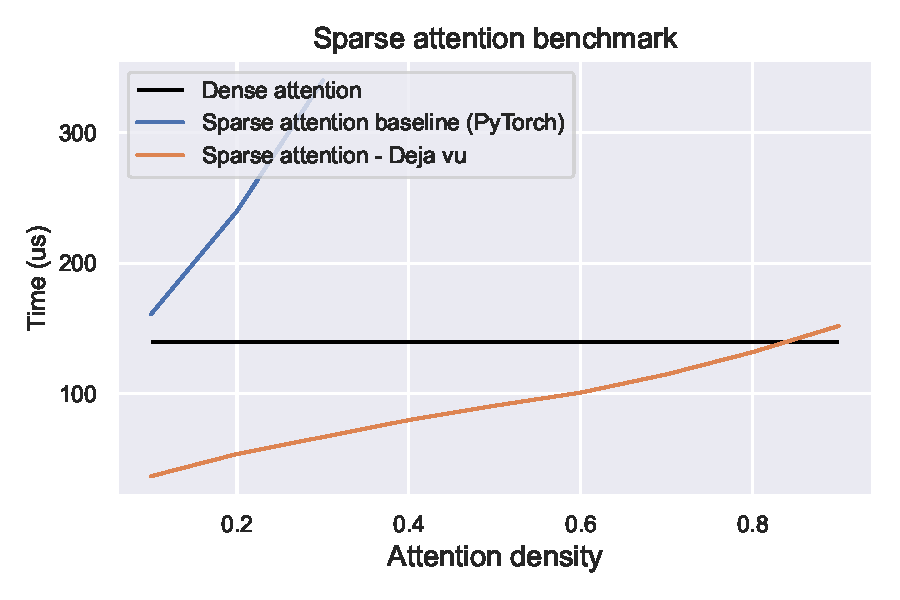
\includegraphics[width=0.8\textwidth]{figure/attn_sparse_speed.pdf}
  \caption{\label{fig:attn_sparse_speed}Speed benchmarking of the attention layer of
    OPT-175B on 8xA100s. Our sparse implementation is up to 5$\times$ faster than
    the baseline implementation in PyTorch. Our sparse attention implementation
    remains faster than dense MLP for density up to 0.8.}
\end{figure}

We validate that our hardware-aware implementation of sparse MLP and sparse
attention (Section~\ref{sec:sparse_matmul}) yields wall-clock speed up compared to both dense MLP/attention and
compared to the standard implementation in PyTorch.

Recall that our implementation fuses the sparse indexing and the multiplication
$(W_{S_M}^1)^\top y$ for weight matrices $(W^1)^\top$ and input vector $y$.
In cases where we need to index $W^2_{S_M}$, we store the transpose of
$W^2$ to ensure memory coalescing.
For the baseline implementation in PyTorch, we index
$(W_{S_M}^1)^\top$ as a separate operation before multiplying with $y$, which
incurs more memory reads/writes. 

Similarly, we fuse the sparse indexing and the multiplication
$(W_{S_A}^Q)^\top y$, $(W_{S_A}^K)^\top y$, $(W_{S_A}^V)^\top y$ for weight matrices $(W^Q)^\top$, $(W^K)^\top$, $(W^V)^\top$ and input vector $y$. Note we usually concatenate all three matrices in the standard implementation, but we separate them here for clarity. In cases where we need to index $W^O_{S_A}$, we store the transpose of
$W^O$ to ensure memory coalescing.

In Figure~\ref{fig:mlp_sparse_speed} and Figure~\ref{fig:attn_sparse_speed}, our
sparse MLP and attention implementations are 4-5$\times$ faster than the baseline
implementation in Pytorch, and remains faster than the dense version for density
up to 0.8.
% \vspace{-4mm}

\section{Notations and Basic Definitions}\label{sec:notation_definition}

For a positive integer $n$, let $[ n ] := \{ 1, 2, \cdots, n\}$. For a matrix $A \in \R^{n \times n}$, let $A_{i, :}$ and $A_{:, j}$ be two column vectors corresponding to the $i$-th row and the $j$-th column of $A$ respectively, and $A_{i, j}$ be the entry at the $i$-th row and the $j$-th column. For a vector $x \in \R^n$, let $\sqrt{x} \in \R^{n}$ denote the vector with the $i$-th entry being $\sqrt{x_i}$ and $\diag ( x ) \in \R^{n \times n}$ denote the diagonal matrix with the $i$-th diagonal entry being $x_i$. For two matrices $A, W \in \R^{n \times n}$, let $\| A \|_W := (\sum_{i=1}^n \sum_{j=1}^n W_{i, j} A_{i, j}^2)^{1/2}$ and $W \circ A$ denote the matrix where $(W \circ A)_{i,j} = W_{i,j} A_{i,j}$. For matrix $W \in \R^{n \times n}$, let $D_{W_i} := \diag( W_{i, :} )$ with $i \in [n]$. 

For two vectors $x \in \R^n$ and $w \in \R^n_{\geq 0}$, let $\| x\|_w := (\sum_{i=1}^n w_i x_i^2)^{1/2}$.   For a vector $x$, we denote $\| x \|_2 := ( \sum_{i=1}^n x_i^2 )^{1/2}$ as its $\ell_2$ norm. We denote $\| x \|_p := (\sum_{i=1}^n |x_i|^p)^{1/p}$ as its $\ell_p$ norm. For a square matrix $A$, we denote $\tr[A]$ as the trace of matrix $A$. 

For a matrix $A \in \R^{n \times k}$ (suppose $n \geq k$), we use $\| A \|$ to denote its spectral norm, i.e., $\| A \| = \sup_{x} \| A x \|_2 / \| x \|_2$. We use $\| A \|_F$ to denote its Frobenius norm $\| A \|_F : = (\sum_{i=1}^n \sum_{j=1}^k A_{i,j}^2 )^{1/2}$.

Suppose matrix $A \in \R^{n \times k}$ has SVD decomposition $U \Sigma V^\top$ where $U \in \R^{n \times k}$ (this matrix has orthonormal columns), $\Sigma \in \R^{k \times k}$ is a diagonal matrix, and $V \in \R^{k \times k}$. We call columns of $U$ are singular vectors. We use $A^\dagger \in \R^{k \times n}$ to denote the Moore-Penrose pseudoinverse, then $A^\dagger = V \Sigma^{-1} U^\top$. Suppose $\Sigma \in \R^{k \times k}$ is sorted diagonal matrix, let $\sigma_1, \cdots, \sigma_k$ denote the diagonal entries of $\Sigma$. Then we call $\sigma_i$ the $i$-th singular value of matrix, and we write it as $\sigma_i(A)$.

For any symmetric matrix $B \in \R^{k \times k}$, we define its eigenvalue decomposition as $U \Lambda U^\top$, where $\Lambda$ is a diagonal matrix. Let $\lambda_1, \cdots, \lambda_k$ denote the entries on diagonal of $\Lambda \in \R^{k \times k}$. We say $\lambda_i$ is the $i$-th eigenvalue. Usually we write it as $\lambda_{i}(B)$.

The connection between eigenvalues and singular values is 
\begin{align*}
\sigma_i^2(A) = \lambda_i (A^\top A)
\end{align*}

We use notation $A \succeq 0$ to denote that matrix $A$ is positive semidefinite (psd). Mathematically, $A\succeq 0$ means for all vectors $x$, we have $x^\top A x \geq 0$.

Similarly, for two squarer matrices $A$ and $B$, we use $A \succeq B$ to denote the case where for all vectors $x$, $x^\top  Ax \geq x^\top B x$. 

We use $\Pr[]$ and $\E[]$ for probability and expectation. We denote $\max\{a,b\}$ as the maximum between $a$ and $b$. We denote $\min \{a,b\}$ (resp. $\max\{a,b\}$) as the minimum (reps. maximum) between $a$ and $b$. 

 Throughout, for non-negative real numbers
a and b, we use the notation $a = (1 \pm \epsilon)b ~\text{if}~a \in [(1 - \epsilon)b,(1 + \epsilon)b]$.

\section{Subspace Embeddings and Norm Preserving}\label{sec:subspace_embedding}
In Section \ref{sec:soft_max_func}, we show the norm preserving of the soft-max functions.
In Section \ref{sec:relu_func}, we show the norm preserving of the ReLU function.
In Section \ref{sec:folded_dist}, we introduce the folded Guassian distribution.
In Section \ref{sec:l2_subspace}, we introduce the $\ell_2$ subspace embedding.
In Section \ref{sec:l1_subspace}, we introduce the $\ell_1$ subspace embedding.
In Section \ref{sec:rand_mat}, we introduce different sketching matrices for subspace embedding.

%\iffalse
%Some useful papers here
%\begin{itemize}
%    \item \cite{lwy21}\href{https://arxiv.org/pdf/2104.12946.pdf}{arxiv link}
%    \item \cite{ww18}\href{https://arxiv.org/pdf/1801.04414.pdf}{arxiv link}
%    \item \cite{swz17}\href{https://arxiv.org/pdf/1611.00898.pdf}{arxiv link}
%    \item \cite{w14}\href{https://arxiv.org/pdf/1411.4357.pdf}{arxiv link}
%\end{itemize}
%\fi
%We use $\phi : \R \rightarrow \R$ to denote ReLU function, i.e., $\phi(z) = \max\{z,0\}$.

\subsection{Soft-Max Functions}\label{sec:soft_max_func}


Let $K \in \R^{s \times d}$ and $V \in \R^{d \times s}$.
Inspired by the softmax unit in the attention scheme of large language models. The softmax related regression has been studied in many settings \cite{zhdk23,as23,bsz23,lsz23,dms23,dls23,gms23,lsx+23,gsy23_dp}. In this work, we follow the standard softmax definition. 
We define $\sigma_1 : \R^s \rightarrow \R^s$ to be a softmax function, i.e., for any vector $y \in \R^s$, the $\sigma(y)$ can be written as
\begin{align*}
\sigma_1( y )_i =  \frac{ \exp(y_i) }{ \sum_{j=1}^d \exp(y_j) } , ~~~ \forall i \in [d]
\end{align*}

The standard softmax is $\ell_1$ version. In this work, we also consider the $\ell_2$ generalization. 
We define $\sigma_2: \R^s \rightarrow \R^s$ to be  a softmax function ($\ell_2$ version), i.e., for any vector $y \in \R^s$, the $\sigma(y)$ can be written as
\begin{align*}
\sigma_2( y )_i =  \frac{ \exp( y_i) }{ ( \sum_{j=1}^d \exp(2 y_j) )^{1/2} } , ~~~ \forall i \in [d]
\end{align*}


We define function $f : \R^d \rightarrow \R^d$
\begin{align}\label{eq:f_x}
f (x) =  V \cdot ( \sigma (K \cdot x) ) 
\end{align}

\begin{definition}
We say ${\cal X} \subset \R^d$ is a rank-$k$ subspace, if there is an orthonormal basis $U \in \R^{d \times k}$, for any $x \in {\cal X}$, there is $ y \in \R^k$ such that
\begin{align*}
x = U y.
\end{align*}
\end{definition}

We can have
\begin{lemma}\label{lem:ell_2_subspace_imply_norm_preserve}
Let $\tau \in (0,1)$. Let ${\cal X} \subset \R^d$ denote a subspace with rank $k$.
Let $f$ be defined based on $\sigma_2$ function. 
Let $\ov{V}$ is a random Gaussian matrices with $d \geq \Omega( \epsilon^{-2} ( k + \log(1/\delta) ))$ rows. Let $V = \tau \ov{V} $, then we have with probability $1-\delta$ 
\begin{align*}
(1-\epsilon) \tau \| x \|_2 \leq \| f(x) \| \leq (1+\epsilon) \tau \| x \|_2.
\end{align*}
for all unit vectors $x \in {\cal X}$.

Further, if $d=  O(k + \log(1/\delta))$, then we have
\begin{align*}
0.5 \tau \| x \|_2 \leq \| f(x) \| \leq 2 \tau \| x \|_2.
\end{align*}
\end{lemma} 
\begin{remark}
The above condition implies that $f$ is a shrinking operator but also not shrinking arbitrarily small.
\end{remark}
\begin{proof}
Given $d \geq \Omega( \epsilon^{-2} ( k + \log(1/\delta) ) )$, by using Lemma~\ref{lem:rand_gauss} 
, we have
\begin{align*}
(1-\epsilon)  \| y \|_2 \leq \| \ov{V} y \|_2 \leq (1+\epsilon)  \| y \|_2
\end{align*}
As the input of the function $f$ here is the output of a softmax function ($\ell_2$ version), we know that $\| y \|_2 = 1$.

Thus, we have
\begin{align*}
(1-\epsilon)  \leq \| \ov{V} y \|_2 \leq (1+\epsilon) 
\end{align*} 
By rescaling $V$, we have
\begin{align*}
(1-\epsilon)  \| x \|_2 \leq \| V y \|_2 \leq (1+\epsilon)   \| x \|_2.
\end{align*} 
\end{proof}


\begin{lemma}
Let $\tau \in (0,1)$. Let ${\cal X} \subset \R^d$ denote a subspace with rank $k$. 
Let $f$ be defined based on $\sigma_1$ function. Suppose $\ov{V}$ is a random Gaussian matrix with $d \geq \Omega( (k + \log(1/\delta)) )$ 
rows. Let $V = \frac{1}{2} \tau \ov{V}$.

Then we have
\begin{align*}
\frac{1}{4\sqrt{s}} \tau \cdot \| x \|_2 \leq \| f( x ) \|_2 \leq  \tau \cdot \| x \|_2
\end{align*}
for all unit vectors $x$.
\end{lemma}
\begin{proof}

By property of subspace embedding, we know that if $d \geq \Omega(\epsilon^{-2} (s+\log(1/\delta)))$,
\begin{align*}
(1-\epsilon) \| y \|_2 \leq \| \ov{V} y \|_2 \leq (1+\epsilon) \| y \|_2
\end{align*}
By property of function of $f$, we know we only need to care $\| y \|_1 = 1$, this implies that %\Tianyi{what is reason for the following step?} \Zhao{Because $y$ has length $s$. The following is true forever. You can try some examples. Then you have a feeling why it's true}
\begin{align*}
\frac{1}{\sqrt{s}} \| y \|_1 \leq \| y \|_2 \leq \| y \|_1
\end{align*}

On one hand, we have
\begin{align}\label{eq:vy_upper}
\| \ov{V} y \|_2 \leq &~  (1+\epsilon) \cdot \| y \|_2 \notag\\
\leq &~  (1+\epsilon) \cdot \| y \|_1 \notag\\
=&~  (1+\epsilon),
\end{align}
where the first step follows from $\| \ov{V} y \|_2 \leq (1+\epsilon) \| y \|_2$, the second step follows from $\| y \|_2 \leq \| y \|_1$ and the last step follows from $\| y \|_1  = 1$.

On the other hand, we have
\begin{align}\label{eq:vy_lower}
\| \ov{V} y \|_2 \geq &~ (1-\epsilon) \| y \|_2 \notag\\
\geq &~  \frac{1}{\sqrt{s}} (1-\epsilon) \| y \|_1 \notag\\
=&~ \frac{1}{\sqrt{s}} (1-\epsilon),
\end{align}
where the first step follows from $(1-\epsilon) \| y \|_2 \leq \| \ov{V} y \|_2 $, the second step follows from $\frac{1}{\sqrt{s}} \| y \|_1 \leq \| y \|_2 $ and the last step follows from $\| y \|_1  = 1$.


Combining Eq.~(\ref{eq:vy_lower})%\Tianyi{the equation notation here is weird, should I just delete Eq.}\Zhao{I think ICML template is funny, you can hard code it as what I do}\Tianyi{fixed}
 and Eq.~(\ref{eq:vy_upper}) together, we have
\begin{align*}
(1-\epsilon) \frac{1}{\sqrt{s}}  \leq \| \ov{V} y \|_2 \leq (1+\epsilon) 
\end{align*} 
Choosing $\epsilon = 1/2$, we have %\Tianyi{the following equation should be $  \frac{1}{2\sqrt{s}}  \leq \| \ov{V} y \|_2 \leq  \frac{3}{2}$}
\begin{align*}
 \frac{1}{2\sqrt{s}}  \leq \| \ov{V} y \|_2 \leq 2.
\end{align*}
By $V = \frac{1}{2} \tau \ov{V}$ and $\|x\|_2 = 1$, we have%\Tianyi{the following equation should be  $\frac{1}{4\sqrt{s}} \tau \| x \|_2 \leq \| V y \|_2 \leq   \frac{3}{4}\tau \| x \|_2.$}
\begin{align*}
\frac{1}{4\sqrt{s}} \tau \| x \|_2 \leq \| V y \|_2 \leq   \tau \| x \|_2.
\end{align*} 

\end{proof}

\subsection{ReLU Functions}\label{sec:relu_func}

We use $\phi : \R \rightarrow \R$ to denote ReLU function, i.e., $\phi(z) = \max\{z,0\}$.

We define function $g : \R^d \rightarrow \R^d$
%%%Zhao: Before this label is {eq:f_x}
\begin{align}\label{eq:g_x}
g (x) =  V \cdot ( \phi (K \cdot x) ) 
\end{align}

Let $K \in \R^{s \times d}$ and $V \in \R^{d \times s}$.

\begin{lemma}
%Let $\tau = 2/d$. 
Let ${\cal X} \subset \R^d$ denote a rank-$k$ subspace. %Let $S$ denote a set of points from ${\cal X} \subset \R^d$ sand $|S| \leq n$. 
Let $K$ denote a random Gaussian matrix. Let $V$ denote a random Gaussian matrix. Let $s \geq \Omega( \epsilon^{-2}  k\log(1/ (\delta \epsilon ) ) )$. Let $d \geq \Omega(\epsilon^{-2} (k + \log(1/\delta)))$. Then we know with high probability $1-\delta$, for all unit vector $x \in {\cal X}$
\begin{align*}
(1-\epsilon) \| x \|_2 \leq \| f(x) \|_2 \leq (1+\epsilon) \| x \|_2
\end{align*}
\end{lemma}
\begin{proof}
Suppose $s \geq \Omega( \epsilon^{-2} \log(1/\delta ) )$.


Using Lemma~\ref{lem:lm}, Fact~\ref{fac:key_property_ReLU}, we can show that for each fixed 
\begin{align*}
(1-\epsilon) \| x \|_2 \leq \| \phi(K x ) \|_2 \leq (1+\epsilon) \| x \|_2
\end{align*}
holds with probability $1-\delta$.

By a standard $\epsilon$-net argument (Lemma~\ref{lem:epsilon_net}), the net points in ${\cal X}$ is at most $(10/\epsilon)^{O(k)}$.


Taking a union bound over all the net points, we can show that for all $x \in {\cal X}$
\begin{align*}
(1-\epsilon) \| x \|_2 \leq \| \phi(K x ) \|_2 \leq (1+\epsilon)\| x \|_2
\end{align*}
holds with probability $1-\delta/2$ and $s \geq \Omega( \epsilon^{-2} k \log(1/ (\delta \epsilon) ) )$.

Further, we using Lemma~\ref{lem:rand_gauss}, we can show that
\begin{align*}
(1-\epsilon) \| \phi(K x) \|_2 \leq \| f(x) \|_2 \leq (1+\epsilon) \| \phi(K x) \|_2
\end{align*}
holds with probability $1-\delta/2$.

Combining together,
\begin{align*}
 (1-\epsilon)^2  \| x \|_2 \leq \| f(x) \|_2 \leq (1+\epsilon)^2 \| x \|_2 
\end{align*}
holds with probability $1-\delta$.

Rescaling the $\epsilon$, we complete the proof.

%Choosing $\epsilon = \Theta(1)$, and setting $\alpha = \Theta(\beta)$, we complete the proof.
\end{proof}

\subsection{Folded Gaussian Distribution}\label{sec:folded_dist}

We state a standard tool from literature,
\begin{lemma}[Lemma 1 on page 1325 of Laurent and Massart \cite{lm00}%, Lemma A.7 in \cite{sy21}
]\label{lem:lm}
    Let $X \sim \mathcal{X}_k^2$ be a chi-squared distributed random variable with $k$ degrees of freedom. Each one has zero means and $\sigma^2$ variance. 
    
    Then,
    \begin{align*}
        \Pr[X - k\sigma^2 \geq (2\sqrt{kt} + 2t) \sigma^2]
        \leq & ~ \exp{(-t)}\\
        \Pr[k\sigma^2 - X \geq 2\sqrt{kt}\sigma^2]
        \leq & ~ \exp{(-t)}
    \end{align*}
    Further if $k \geq \Omega(\epsilon^{-2} t)$ and $t \geq \Omega(\log(1/\delta))$, then we have
    \begin{align*}
    \Pr[ | X - k \sigma^2 | \leq \epsilon k \sigma^2 ] \leq \delta.
    \end{align*}
\end{lemma}

We prove the following property,
\begin{fact}\label{fac:key_property_ReLU}
Let $h, q \in \R^p$ be fixed vectors and $h \neq 0, W \in \R^{m \times p}$ be random matrix with i.i.d. entries $W_{i, j} \sim \mathcal{N} (0, \frac{2}{m} )$, and vector $v \in \R^m$ defined as $v_i=\phi ((W h)_i )=\mathbf{1}_{(W(h+q))_i \geq 0}(W h)_i$. Then,
\begin{itemize}
    \item $ |v_i |$ follows i.i.d. from the following distribution: with half probability $ |v_i |=0$, and with the other half probability $ |v_i |$ follows from folded Gaussian distributions $ |\mathcal{N} (0, \frac{2\|h\|^2}{m} ) |$.
    \item $\frac{m\|v\|^2}{2\|h\|^2}$ is in distribution identical to $\chi_\omega^2$ (chi-square distribution of order $\omega$ ) where $\omega$ follows from binomial distribution $\mathcal{B}(m, 1 / 2)$.
\end{itemize}

\end{fact}

\begin{proof}
    We assume each vector $W_i$ is generated by first generating a gaussian vector $g \sim \mathcal{N} (0, \frac{2   I}{m} )$ and then setting $ W_i=\pm g$ where the sign is chosen with half-half probability. Now, $ | \langle W_i, h \rangle |=|\langle g, h\rangle|$ only depends on $g$, and is in distribution identical to $ |\mathcal{N} (0, \frac{2\|h\|^2}{m} ) |$. Next, after the sign is determined, the indicator $\mathbf{1}_{ \langle W_i, h+q \rangle \geq 0}$ is $1$ with half probability and $0$ with another half. Therefore, $ |v_i |$ satisfies the aforementioned distribution. As for $\|v\|^2$, letting $\omega \in\{0,1, \ldots, m\}$ be the variable indicator how many indicators are $1$ , then $\omega \sim \mathcal{B}(m, 1 / 2)$ and $\frac{m\|v\|^2}{2\|h\|^2} \sim \chi_\omega^2$.
\end{proof}
 

\subsection{$\ell_2$ subspace embedding}\label{sec:l2_subspace}

We define a standard notion in sketching technique.\footnote{We remark that sketching technique has widely applied to many applications such as linear regression, low-rank approximation \cite{cw13,nn13,ldfu13,bwz16,c16,rsw16,swz17,swz19}, linear programming \cite{sy21,dly21,jswz21,gs22}, semi-definite programming \cite{gs22,syyz23}, empirical risk minimization\cite{lsz19,qszz23}, training over-parameterized neural network \cite{bpsw21,szz21,als+22,hswz22,z22}.}
\begin{definition}[$\ell_2$ subspace embedding \cite{s06}]\label{def:l2_subspace_embedding}%\cite{w+14}
A $(\epsilon, \delta, \ell_2)$-subspace embedding for the column space of an $n \times d$ matrix $A$ is a matrix $S$ for which %for which all $x \in \R^d$
\begin{align*}
  \Pr [ \forall x \in \mathbb{R}^d,  \|S Ax\|_2^2 = (1 \pm \epsilon) \|Ax\|_2^2 ] \geq 1-\delta.
\end{align*}
%holds with probability $1-\delta$.
The above condition is equivalent to
\begin{align*}
\Pr[ \| U^\top U - U^\top S^\top S U \| \leq \epsilon ] \geq 1-\delta.
\end{align*}
where the $U$ is the orthonormal basis of $A$.
\end{definition}
For the reason of above conditions are equivalent, we refer the readers to the survey \cite{w14}.

We state a standard tool in literature,
\begin{lemma}[Lemma 5 in \cite{w14}]\label{lem:epsilon_net}
Let ${\cal X} \subset\R^d$ be rank $k$. For any $\gamma \in (0,1)$, there is a $\gamma$-net $N$ of ${\cal X}$ for which $|N| \leq (1+4 /\gamma)^k$.
\end{lemma}

\subsection{$\ell_1$ subspace embedding}\label{sec:l1_subspace}

 When $p=1$, using Cauchy random variables, Sohler and Woodruff \cite{sw11} showed there exist $\ell_1$ oblivious subspace embeddings with $O(d \log d)$ rows and $\kappa=O(d \log d)$. This approach was generalized by using $p$-stable random variables in work of Meng and Mahoney \cite{mm13} to $\ell_p$-norms when $1<p<2$, where they showed there exist $\ell_p$ oblivious subspace embeddings with $O(d \log d)$ rows and $\kappa=O ((d \log d)^{1 / p} )$. Unlike the case when $p=2$, due to the large distortion

% Previous impossibility results for dimension reduction in $\ell_1$ \cite{ln04,bc05,cs02} are established by creating a set of $O(n)$ points in $\R^n$ and showing that any (non-oblivious) embedding on them incurs a large distortion. In this paper, we focus on embedding a $d$-dimensional subspace of $\R^n$ into $\R^{\text {poly }(d)}$ using oblivious embeddings. We stress that $O(n)$ points in a $d$-dimensional subspace have a very different structure from $O(n)$ arbitrary points in $\R^n$. Previous results \cite{cp15} showed that any $d$-dimensional subspace in $\R^n$ can be embedded into $\R^{O (d(\log d) \epsilon^{-2} )}$ with $(1+\epsilon)$ distortion in $\ell_1$ using non-oblivious linear embeddings, where $\epsilon>0$ is an arbitrarily small constant. Here the subspace structure is critically used, since Charikar and Sahai \cite{cs02} showed that there exist $O(n)$ points such that any linear embedding $\R^n \rightarrow \R^d$ must incur a distortion of $\Omega(\sqrt{n / d})$, even for non-oblivious linear embeddings.

 In \cite{ww18}, they show for every $1 \leq p<2$, any oblivious subspace embedding with dimension $r$ has distortion $\kappa=\Omega (\frac{1}{ (\frac{1}{d} )^{1 / p} \cdot \log ^{2 / p} r+ (\frac{r}{n} )^{1 / p-1 / 2}} )$. 
 They also give sparse oblivious subspace embeddings for every $1 \leq p<2$ which are optimal in dimension and distortion, up to poly $(\log d)$ factors. Importantly for $p=1$, they achieve $r=O(d \log d), \kappa=O(d \log d)$ and $s=O(\log d)$ non-zero entries per column. 

\begin{definition}[$\ell_1$ subspace embedding]\label{def:l1_subspace_embedding}%\cite{w+14}
Let $0< \alpha < \beta$ be parameters. We will say a matrix $S$ is an $\ell_1$ subspace embedding for an $n \times d$ matrix $A$ if there are constants $c_1, c_2 > 0$ so that for all $x \in \R^{d}$,
\begin{align*}
    \|Ax\|\leq \|SAx\|_1 \leq d^{c_1} \|Ax\|_1,
\end{align*}
and $S$ has at most $d^{c_2}$ rows.
\end{definition}

%\begin{lemma}
%Suppose that $A \in \R^{d \times d}$ is random matrix, and $\|y \|_1=1$, we want to show that
%\begin{align*}
%\| A y \|_1 \approx (1\pm \epsilon) \| y \|_1
%\end{align*}
%\end{lemma}
\subsection{Random Matrices}\label{sec:rand_mat}


\begin{table*}[!ht]
    \centering
\begin{tabular}{|c|l|l|l|}
\hline {\bf Matrices} & $b$ & {\bf Time for} $R \cdot A$ & {\bf Reference} \\
\hline Random Gaussian & $\epsilon^{-2}(d+\log (1 / \delta))$ & $\Tmat(b, n, d)$ & Thm. 6 of \cite{w14} \\
\hline SRHT & $\epsilon^{-2}(\sqrt{d}+\sqrt{\log n})^2 \log (d / \delta)$ & $n d \log  (\epsilon^{-1} d(\log n) )$ & Thm. 7 of \cite{w14} \\
\hline AMS & $\epsilon^{-2}(d+\log (1 / \delta))$ & $\Tmat(b, n, d)$ & Follow from JL guarantee \\
\hline Count-sketch & $\epsilon^{-2} \delta^{-1} d^2$ & $\mathrm{nnz}(A)$ & Thm. 9 of \cite{w14} \\
\hline Sparse embedding & $\epsilon^{-2} d \cdot$ poly $\log (d /(\epsilon \delta))$ & $\epsilon^{-1} \mathrm{nnz}(A)$ poly $\log (d /(\epsilon \delta))$ & Thm. 10 (2) of \cite{w14} \\
\hline Sparse embedding& $\epsilon^{-2} d^{1+\gamma}$ & $\epsilon^{-1} \mathrm{nnz}(A) \operatorname{poly}(1 / \gamma)$ & Thm. 10 (1) of \cite{w14} \\
\hline
\end{tabular}
\caption{Summary for different sketching matrices for subspace embedding. The sketching matrix $R$ has size $b \times n$. The vectors are from the column subspace of matrix $A$ with size $n \times d . \epsilon \in(0,1)$ is the error parameter, and $\delta \in(0,1)$ is the probability parameter. $\mathcal{T}_{\text {mat }}(a, b, c)$ denotes the running time of fast matrix multiplication of two matrices with size $a \times b$ and $b \times c .$ In the first sparse embedding matrix, each column has $s \geq \epsilon^{-1}$ poly $\log (d /(\epsilon \delta))$ non-zero entries;  In the second sparse embedding matrix, each column has $s \geq \epsilon^{-1}$ poly $(1 / \gamma)$ non-zero entries, $\gamma>0$ is a tunable parameter that gives different trade-offs, and $\delta$ can be as small as $1 /$ poly $(d).$ For count-sketch matrices, the subspace embedding guarantee is proved from JL moment property, instead of directly from JL guarantee.}
\label{tab:summary_sketching}
\end{table*}

\begin{lemma}[Theorem 6 of \cite{w14}]\label{lem:rand_gauss}
    Let $0<\epsilon, \delta <1$ and $S=\frac{1}{\sqrt{k}}   R \in \R^{k \times n}$ where the entries $  R_{i, j}$ of $  R$ are independent standard normal random variables. Then if $k=$ $\Theta (\epsilon^{-2}(d+\log (1 / \delta))  )$, then for any fixed $n \times d$ matrix $A$, with probability $1-\delta, S$ is a $(1 \pm \epsilon) \ell_2$-subspace embedding for $A$, that is, simultaneously for all $x \in \R^d, \| S A x\|_2=(1 \pm \epsilon)\|A x\|_2$. Here $C>0$ is an absolute constant.
\end{lemma}


We consider several standard sketching matrices:
\begin{enumerate}
    \item Random Gaussian matrices.
    \item Subsampled randomized Hadamard/Fourier transform (SRHT) matrices \cite{ldfu13}.
    \item AMS sketch matrices \cite{ams96}, random $\{-1,+1\}$ per entry.
    \item Count-Sketch matrices \cite{ccf02}, each column only has one non-zero entry, and is $-1,+1$ half probability each.
    \item Sparse embedding matrices \cite{nn13}, each column only has $s$ non-zero entries, and each entry is $-\frac{1}{\sqrt{s}},+\frac{1}{\sqrt{s}}$ half probability each.
    \item Uniform sampling matrices.
\end{enumerate}

\begin{definition}[Random Gaussian matrix]
    We say $R \in \R^{b \times n}$ is a random Gaussian matrix if all entries are sampled from $\mathcal{N}(0,1 / b)$ independently.
\end{definition}

\begin{definition}[Subsampled randomized Hadamard/Fourier transform matrix \cite{ldfu13}]
    We say $R \in \R^{b \times n}$ is a subsampled randomized Hadamard transform (SRHT) matrix \footnote{ In this case, we require  $\log n$  o be an integer. } if it is of the form $R=\sqrt{n / b} S H D$, where $S \in \R^{b \times n}$ is a random matrix whose rows are b uniform samples (without replacement) from the standard basis of $\R^n, H \in \R^{n \times n}$ is a normalized Walsh-Hadamard matrix, and $D \in \R^{n \times n}$ is a diagonal matrix whose diagonal elements are i.i.d. Rademacher random variables.
\end{definition}

\begin{definition}[AMS sketch matrix \cite{ams96}]
   Let $h_1, h_2, \cdots, h_b$ be $b$ random hash functions picking from a 4-wise independent hash family $\mathcal{H}=\{h:[n] \rightarrow\{-\frac{1}{\sqrt{b}},+\frac{1}{\sqrt{b}}\}\}$. Then $R \in \R^{b \times n}$ is a AMS sketch matrix if we set $R_{i, j}=h_i(j)$
\end{definition}

\begin{definition}[Count-sketch matrix \cite{ccf02}]
    Let $h:[n] \rightarrow[b]$ be a random 2-wise independent hash function and $\sigma:[n] \rightarrow\{-1,+1\}$ be a random 4-wise independent hash function. Then $R \in \R^{b \times n}$ is a count-sketch matrix if we set $R_{h(i), i}=\sigma(i)$ for all $i \in[n]$ and other entries to zero.
\end{definition}

\begin{definition}[Sparse embedding matrix I \cite{nn13}]
    We say $R \in \R^{b \times n}$ is a sparse embedding matrix with parameter $s$ if each column has exactly $s$ non-zero elements being $\pm 1 / \sqrt{s}$ uniformly at random, whose locations are picked uniformly at random without replacement (and independent across columns) \footnote{For our purposes the signs need only be $O(\log d)$-wise independent, and each column can be specified by a $O(\log d)$-wise independent permutation, and the seeds specifying the permutations in different columns need only be $O(\log d)$-wise independent.}.
\end{definition}

\begin{definition}[Sparse embedding matrix II \cite{nn13}]
   Let $h:[n] \times[s] \rightarrow[b / s]$ be a random 2-wise independent hash function and $\sigma:[n] \times[s] \rightarrow\{-1,1\}$ be a 4-wise independent. Then $R \in \R^{b \times n}$ is a sparse embedding matrix II with parameter $s$ if we set $R_{(j-1) b / s+h(i, j), i}=\sigma(i, j) / \sqrt{s}$ for all $(i, j) \in[n] \times[s]$ and all other entries to zero \footnote{This definition has the same behavior as sparse embedding matrix I for our purpose}.
\end{definition}

\begin{definition}[Uniform sampling matrix]
    We say $R \in \R^{b \times n}$ is a uniform sampling matrix if it is of the form $R=\sqrt{n / b} S D$, where $S \in \R^{b \times n}$ is a random matrix whose rows are b uniform samples (without replacement) from the standard basis of $\R^n$, and $D \in \R^{n \times n}$ is a diagonal matrix whose diagonal elements are i.i.d. Rademacher random variables.
\end{definition}



%The above is only one layer, do we need multiple layer.
\section{Distances, Angles, and Inner Product}\label{sec:distances_angles}

Most of the properties in this section are very standard in literature, e.g., see \cite{gsyz23}.

Let $U \in \R^{n \times k}$ denote an orthonormal basis, we use $U_{\bot} \in \R^{n \times (n-k)}$ denote the matrix such that $U U^\top + U_{\bot} U_{\bot}^\top = I_n$.


\begin{definition}\label{def:angle_and_distance}
Let $X \in \R^{n \times k}$ and $Y \in \R^{n \times k}$.

For any matrix $X$, and for orthogonal matrix $Y$ ($Y^\top Y = I_k$) we define
%\Tianyi{what is the definition of $A_\bot$} \Zhao{See above}
\begin{itemize}
    \item $\tan \theta(Y,X) := \| Y_{\bot}^\top X ( Y^\top X )^{-1} \|$
\end{itemize}
For orthogonal matrices $Y$ and $X$ ($Y^\top Y = I_k$ and $X^\top X = I_k$), we define %\Tianyi{what is $\sigma$} \Zhao{Read notation section}
\begin{itemize}
    \item $\cos \theta (Y,X) := \sigma_{\min} (Y^\top X)$. 
    \begin{itemize} 
        \item It is obvious that $\cos (Y,X) = 1/ \| (Y^\top X)^{-1} \|$ and $\cos(Y,X) \leq 1$.
    \end{itemize}
    \item $\sin \theta(Y,X) := \| (I - Y Y^\top) X \|$.
    \begin{itemize} 
        \item It is obvious that $\sin \theta(Y,X) = \| Y_{\bot} Y_{\bot}^\top X \| = \| Y_{\bot}^\top X \|$ and $\sin \theta(Y,X) \leq 1$.
    \end{itemize}
    \item $\dist(Y,X) := \min_{Q \in O_k} \| YQ - X \|$
\end{itemize}  
where $O_k$ is the set of $k \times k$ orthogonal matrices. 
\end{definition}

\begin{lemma}[Structural lemma for orthogonal matrices]
\label{lem:trig_structural}
Let $X, Y\in \R^{n\times k}$ be orthogonal matrices. Then
\begin{align*}
    (Y^\top X)_\bot = & ~ Y_\bot^\top X.
\end{align*}
\end{lemma}

\begin{proof}
    Let us first compute the Gram of $Y^\top X$, which is
\begin{align*}
    X^\top YY^\top X 
    = & ~ X^\top (I-Y_\bot Y_\bot^\top) X \\
    = & ~ X^\top X-X^\top Y_\bot Y_\bot^\top X \\
    = & ~ I_k-X^\top Y_\bot Y_\bot^\top X,
\end{align*}
where the first step follows from $Y_\bot Y_\bot^\top + YY^\top = I$, the second step follows from simple algebra, and the last step follows from $X$ is an orthogonal matrix, so $X^\top = X^{-1}$.

This means that $(Y^\top X)_\bot=Y_\bot^\top X$.
\end{proof}

\begin{lemma}[Orthogonal and inverse share singular vectors]
\label{lem:perp_inv_singular}
Let $A\in \R^{k\times k}$ be non-singular, then $A_\bot$ and $A^{-1}$ have the same set of singular vectors. Consequently, $\|A_\bot A^{-1}\|=\|A_\bot\|\|A^{-1}\|$. 

\end{lemma}

\begin{proof}
     Let $A\in \R^{k\times k}$ and $A^\top A+A_\bot^\top A_\bot=I_k$, we will show that $\|A_\bot A^{-1}\|=\|A_\bot \| \|A^{-1}\|$. Let $x\in \R^k$ be the unit eigenvector of $A$ that realizes the spectral norm, note that
\begin{align*}
    \|A_\bot x\|_2^2 = & ~ 1-\|A\|^2,
\end{align*}
we argue that $x$ corresponds to the smallest singular value of $A_\bot$ via contradiction. Suppose there exists some unit vector $y$ with $\|A_\bot y\|_2 < \|A_\bot x\|_2$, by definition, we know that $\|A_\bot y\|_2^2+\|Ay\|_2^2=1$, this means that $\|Ay\|_2>\|Ax\|_2=\|A\|$, contradicts the definition of spectral norm. Similarly, if $z$ is the unit vector that realizes the spectral norm of $A_\bot$, then it is also singular vector corresponds to the smallest singular value of $A$, or equivalently, the spectral norm of $A^{-1}$. Our above argument essentially implies that $A_\bot$ and $A^{-1}$ have the same set of singular vectors. The proof is then straightforward: suppose $A_\bot z=\lambda z$ and $A^{-1}z=\mu z$, then
\begin{align*}
    A_\bot A^{-1} z 
    = & ~ A_\bot \mu z \\
    = & ~ \mu (A_\bot z) \\
    = & ~ \lambda \mu z,
\end{align*}
where the first step follows from our assumption, the second step follows from $\mu$ is a real number and a real number multiplying a matrix is commutative and follows from the associative property, and the third step follows from our assumption.

Thus, we have $\|A_\bot A^{-1}\|=\|A_\bot\|\|A^{-1}\|$, and we have proved the assertion.
\end{proof}

\begin{lemma}\label{lem:tan_is_sin_cos}
Let $X, Y\in \R^{n\times k}$ be orthogonal matrices, then 
\begin{align*}
    \tan \theta(Y,X) = & ~ \frac{\sin \theta(Y,X)}{\cos \theta(Y,X)}.
\end{align*}
\end{lemma}


\begin{proof}
Due to Lemma~\ref{lem:trig_structural}, we have $(Y^\top X)_\bot=Y^\top_\bot X$. Thus, $\tan\theta(Y,X)=\|(Y^\top X)_\bot (Y^\top X)^{-1}\|$. The proof then follows straightforwardly from Lemma~\ref{lem:perp_inv_singular}.
\end{proof}

\begin{lemma}\label{lem:sin^2_and_cos^2_is_1}
Let $X, Y\in \R^{n\times k}$ be orthogonal matrices, then $\sin^2\theta(Y, X) + \cos^2\theta(Y,X) =1$.
\end{lemma}
\begin{proof}
Recall that $\cos\theta(Y,X)=\frac{1}{\|(Y^\top X)^{-1}\|}$ and $\sin\theta(Y,X)=\|Y_\bot^\top X\|$, by Lemma~\ref{lem:trig_structural}, we know that $(Y^\top X)_\bot=Y^\top_\bot X$, therefore $\sin\theta(Y,X)=\|(Y^\top X)_\bot \|$. Let $A:=Y^\top X$, by Lemma~\ref{lem:perp_inv_singular}, we know that $A_\bot$ and $A^{-1}$ have the same singular vectors, or equivalently, the singular vector realizing $\|A_\bot\|$ corresponds to the smallest singular value of $A$. Let $z\in \R^k$ be the unit singular vector with singular value $\|A_\bot\|$, then
\begin{align*}
    z^\top A^\top Az+z^\top A_\bot^\top A_\bot z = & ~ 1, \\
    \|A_\bot\|^2+\sigma_{\min}^2(A) = & ~ 1, \\
    \cos^2\theta(Y,X)+\sin^2\theta(Y,X) = & ~ 1.
\end{align*}
This completes the proof.
\end{proof}


\subsection{Angle is close}

\begin{lemma}
Let $\epsilon \in (0,0.1)$
Let $x$ denote a unit vector, i.e., $\| x \|_2 = 1$.

Let $z = (x+y) / \| x + y\|_2$.

If $ \| y \|_2 \leq \epsilon \cdot \| x \|_2$, then
\begin{align*}
\sqrt{1-\langle x, z \rangle^2} \leq 2 \sqrt{\epsilon} 
\end{align*}
\end{lemma}
\begin{proof}
We have
\begin{align*}
 \| x + y \|_2 
 \geq & ~\| x \|_2 - \| y \|_2 \\
\geq & ~ 1- \epsilon
\end{align*}
where the first step follows from triangle inequality.

We also have
\begin{align}\label{eq:x_y_bound}
 \| x + y \|_2 
 \leq & ~\| x \|_2 + \| y \|_2 \notag \\
\leq & ~ 1 + \epsilon
\end{align}


We have
\begin{align}\label{eq:1_minus_eps}
(1- \epsilon)^2 \geq 1- 2\epsilon
\end{align}

We also have
\begin{align}\label{eq:1_plus_eps}
\frac{1}{(1+\epsilon)^2} \geq 1- 3 \epsilon
\end{align}
where $\epsilon \in (0,0.1)$.



Combining Eq.~(\ref{eq:1_minus_eps}) and Eq.~(\ref{eq:1_plus_eps}), we have
\begin{align}\label{eq:1_2eps}
\frac{1}{(1+\epsilon)^2} \cdot ( 1 - \epsilon )^2 \geq &~ (1-2\epsilon) \cdot (1-3 \epsilon) \notag\\
=&~ 1 -5 \epsilon + 6 \epsilon^2 \notag\\
\geq &~  1 - 5\epsilon + \epsilon \notag\\
=&~ 1 - 4 \epsilon 
\end{align}
where the first step follows from Eq.~(\ref{eq:1_minus_eps}) and Eq.~(\ref{eq:1_plus_eps}) and the rest of them follow from simple algebra.


Finally, we have
\begin{align*}
1 - \langle x, z \rangle^2
= & ~ 1 - \langle x, \frac{x+y}{ \| x + y \|_2 } \rangle^2 \\
= & ~ 1 - \frac{1}{\| x + y \|_2^2} \langle x , x+y \rangle^2 \\
= & ~ 1 - \frac{1}{\| x + y \|_2^2} \cdot ( \| x \|_2^2 + \langle x , y \rangle )^2 \\
= & ~  1 - \frac{1}{\| x + y \|_2^2} \cdot ( 1 + \langle x , y \rangle )^2 \\
\leq & ~ 1 - \frac{1}{(1+\epsilon)^2} \cdot ( 1 + \langle x , y \rangle )^2 \\
\leq & ~ 1 - \frac{1}{(1+\epsilon)^2} \cdot ( 1 - \epsilon )^2 \\
\leq & ~ 1 -  (1- 4 \epsilon) \\
= & ~ 4 \epsilon,
\end{align*}
where the first step follow the definition of $z$, the second step follows from the reorganization, the third step follows from the definition of inner product, the fourth step follows from $\| x \|_2 = 1$, the fifth step follows from Eq.~(\ref{eq:x_y_bound}), the sixth step follows from  $1+\langle x,y\rangle \geq 1 - | \langle x , y \rangle | \geq 1 - \| x \|_2 \cdot \| y \|_2 \geq 1- \epsilon$, the seventh step follows from Eq.~(\ref{eq:1_2eps}) and the last step follows from simple algebra.


\end{proof}
%Check if $\| f(x) + x \|_2 \approx(1 \pm \epsilon) \| x \|_2$, then cosin is good.

\section{Function Approximations}\label{sec:function_approx}

% \Zhao{Write a roadmap}
We first we show the function approximation for two operators in Section \ref{sec:fun_app_app}, which means that there are two functions. Then we show the function approximations for four operators in Section \ref{sec:fun_app_operators_app}.


\subsection{Function Approximations for Two Operators}\label{sec:fun_app_app}

\begin{lemma}
Let $f_1 : \R^d \rightarrow \R^d$ and let $f_2 : \R^d \rightarrow \R^d$.

Assume the the following conditions
\begin{itemize}
    \item Condition 1a. $f_1$ is a linear function 
    \item Condition 1b. $\| f_1(x) \|_2 \leq \epsilon_1 \| x \|_2$ ($f_1$ is shrinking)
    \item Condition 1c. $\| f_1 (x)  -f_1(y) \|_2 \leq L_1 \| x - y \|_2$ ($f_1$ is Lipschitz)
    \item Condition 2a. $f_2$ is a linear function 
    \item Condition 2b. $\| f_2(x) \|_2 \leq \epsilon_2 \| x \|_2$  ($f_2$ is shrinking)
    \item Condition 2c. $\| f_2 (x)  -f_2(y) \|_2 \leq L_2 \| x - y \|_2$ ($f_2$ is Lipschitz)
\end{itemize}

We define three functions
\begin{itemize}
\item 
\begin{align*}
g_1 (x) = : & ~ (I + f_1) \cdot (I + f_2) (x)  \\
= & ~ x + f_2(x) + f_1 ( x + f_2(x) )
\end{align*}
\item
\begin{align*}
g_2 (x) = : & ~ (I + f_2) \cdot (I + f_1) (x)  \\
= & ~ x + f_1(x) + f_2 ( x + f_1(x) )
\end{align*}
\item
\begin{align*}
g_3 (x) = : & ~ (I + f_1 + f_2) (x)  \\
= & ~ x + f_1(x) + f_2(x)
\end{align*}
\end{itemize}
Then we can show that
\begin{itemize}
    \item Part 1. $\| g_1 (x) - g_2 (x) \|_2 \leq 2 \epsilon_1 \epsilon_2 \| x \|_2$(if $f_1$ and $f_2$ are linear functions)
    \item Part 2. $\| g_1 (x) - g_2 (x) \|_2 \leq (\epsilon_2 \cdot L_1+ \epsilon_1 \cdot L_2) \| x \|_2  $  (if $f_1$ and $f_2$ are Lipschitz functions)
    \item Part 3. $\| g_1 (x) -g_3 (x) \|_2 \leq \epsilon_1 \epsilon_2 \| x \|_2$ (if $f_1$ is a linear function)
    \item Part 4. $\| g_1 (x) -g_3 (x) \|_2 \leq \epsilon_2 \cdot L_1 \| x \|_2$ (if $f_1$ is a Lipschitz function)
    \item Part 5.  $\| g_2 (x) -g_3 (x) \|_2 \leq \epsilon_1 \epsilon_2 \| x \|_2$ (if $f_2$ is a linear function)
    \item Part 6. $\| g_2 (x) -g_3 (x) \|_2 \leq \epsilon_1 \cdot L_2 \| x \|_2$ (if $f_2$ is a Lipschitz function)
\end{itemize}
\end{lemma}
\begin{proof}

{\bf Part 1.}



We have 
\begin{align*}
\| g_1 (x) - g_2 (x) \|_2 \leq &~ \|g_1(x) - g_3(x) \|_2 + \|g_3(x) - g_2(x)\|_2\\
\leq &~   \epsilon_1 \epsilon_2 \| x \|_2 + \epsilon_1 \epsilon_2 \| x \|_2 \\
= &~  2 \epsilon_1 \epsilon_2 \| x \|_2
\end{align*}
where the first step follows from triangular inequality, the second step follows from Part 3 and Part 5 and the last step follows from simple algebra.

{\bf Part 2.}

We have 
\begin{align*}
\| g_1 (x) - g_2 (x) \|_2 \leq &~ \|g_1(x) - g_3(x) \|_2 + \|g_3(x) - g_2(x)\|_2\\
\leq &~  \epsilon_2 \cdot L_1 \| x \|_2+ \epsilon_1 \cdot L_2 \| x \|_2 \\
= &~  (\epsilon_2 \cdot L_1+ \epsilon_1 \cdot L_2) \| x \|_2 
\end{align*}
where the first step follows from triangular inequality, the second step follows from Part 4 and Part 6 and the last step follows from simple algebra.



{\bf Part 3.}

We have 
\begin{align*}
\| g_1 (x) - g_3(x) \|_2
= & ~ \| f_1(x+ f_2(x) ) - f_1(x) \|_2 \\
= & ~ \| f_1 (x+ f_2(x) - x) \|_2 \\
= & ~ \| f_1 (f_2(x) ) \|_2 \\
\leq & ~ \epsilon_1 \cdot \| f_2(x) \|_2 \\
\leq & ~ \epsilon_1 \cdot \epsilon_2 \cdot \| x \|_2,
\end{align*}
where the first step follows from the definition of $g_1$ and $g_3$, the second step follows from the fact that $f_1$ is a linear function, the third step follows from simple algebra, the fourth step follows from Condition 1b and the last step follows from Condition 2b.

{\bf Part 4.}

\begin{align*}
\| g_1 (x) - g_3(x) \|_2
= & ~ \| f_1(x+ f_2(x) ) - f_1(x) \|_2 \\
\leq & ~L_1 \cdot \| x+ f_2(x) - x \|_2  \\
= & ~  L_1 \cdot \| f_2 (x) \|_2 \\
\leq & ~ L_1 \cdot \epsilon_2 \| x \|_2,
\end{align*}
where the first step follows from definition of $g_1$ and $g_3$, the second step follows from Condition 1c, the third step follows from simple algebra and the last step follows from Condition 2b. 
\end{proof}

{\bf Part 5.}

We have 
\begin{align*}
\| g_2 (x) - g_3(x) \|_2
= & ~ \| f_2(x+ f_1(x) ) - f_2(x) \|_2 \\
= & ~ \| f_2 (x+ f_1(x) - x) \|_2 \\
= & ~ \| f_2 (f_1(x) ) \|_2 \\
\leq & ~ \epsilon_2 \cdot \| f_1(x) \|_2 \\
\leq & ~ \epsilon_2 \cdot \epsilon_1 \cdot \| x \|_2,
\end{align*}
where the first step follows from the definition of $g_2$ and $g_3$, the second step follows from the fact that $f_2$ is a linear function, the third step follows from simple algebra, the fourth step follows from Condition 2b and the last step follows from Condition 1b.

{\bf Part 6.}

\begin{align*}
\| g_2 (x) - g_3(x) \|_2
= & ~ \| f_2(x+ f_1(x) ) - f_2(x) \|_2 \\
\leq & ~L_2 \cdot \| x+ f_1(x) - x \|_2  \\
= & ~  L_2 \cdot \| f_1 (x) \|_2 \\
\leq & ~ L_2 \cdot \epsilon_1 \| x \|_2,
\end{align*}
where the first step follows from definition of $g_1$ and $g_3$, the second step follows from Condition 2c, the third step follows from simple algebra and the last step follows from Condition 1b. 

\subsection{Function Approximations for Four Operators}\label{sec:fun_app_operators_app}

\begin{lemma}
For each $i \in [4]$, we assume the following conditions
\begin{itemize}
    \item i(a) $f_i$ is a linear function
    \item i(b) $\| f_i(x) \|_2 \leq \epsilon_i \| x \|_2$ ($f_i$ is shriking)
    \item i(c)  $\| f_i(x) - f_i(y) \|_2 \leq L_i \| x-y\|_2$ ($f_i$ is Lipschitz)
\end{itemize}
We define three functions
\begin{itemize}
    \item $g_1(x):= (I+ f_1) \cdot (I + f_2) \cdot (I + f_3) \cdot (I + f_4) (x)$
    \item $g_2(x): = (I+ f_1) \cdot (I + f_3) \cdot (I + f_2) \cdot (I + f_4) (x)$
    \item $g_3(x) := (I + f_1 + f_2 + f_3 + f_4) (x)$
\end{itemize}
Then, we can show that
\begin{itemize}
    \item Part 1. $\| g_1 (x) - g_2 (x ) \|_2 \leq 2 ( \epsilon_1 \epsilon_2+ \epsilon_1 \epsilon_3 + \epsilon_1 \epsilon_4
        +\epsilon_2\epsilon_3+ \epsilon_2 \epsilon_4
        +\epsilon_3 \epsilon_4 
         + \epsilon_1 \epsilon_2 \epsilon_3 + \epsilon_1 \epsilon_2 \epsilon_4 + \epsilon_1 \epsilon_3 \epsilon_4 +\epsilon_2 \epsilon_3 \epsilon_4 + \epsilon_1 \epsilon_2 \epsilon_3 \epsilon_4) \|x\|_2$ (if $f_i,~\forall i \in [4]$ are linear functions)
    \item Part 2. $\| g_1 (x) - g_2 (x ) \|_2  \leq (2L_1 \epsilon_2  + 2L_1 \epsilon_3  +2L_1 \epsilon_4   +
        L_2 \epsilon_3  + 2L_2  \epsilon_4  + 2L_3  \epsilon_4  +
        2L_1 \epsilon_2 \epsilon_3  +2L_1 \epsilon_2 \epsilon_4   +2L_1 \epsilon_3 \epsilon_4 +
         L_2 \epsilon_3 \epsilon_4  +
        2L_1 \epsilon_2 \epsilon_3 \epsilon_4 + 
         L_3 \epsilon_2 +
          L_3 \epsilon_2 \epsilon_4) \| x\|_2$ (if $f_i,~\forall i \in [4]$ are Lipschitz functions)
    \item Part 3. $\| g_1 (x) - g_3 (x ) \|_2 \leq ( \epsilon_1 \epsilon_2+ \epsilon_1 \epsilon_3 + \epsilon_1 \epsilon_4
        +\epsilon_2\epsilon_3+ \epsilon_2 \epsilon_4
        +\epsilon_3 \epsilon_4 
         + \epsilon_1 \epsilon_2 \epsilon_3 + \epsilon_1 \epsilon_2 \epsilon_4 + \epsilon_1 \epsilon_3 \epsilon_4 +\epsilon_2 \epsilon_3 \epsilon_4 + \epsilon_1 \epsilon_2 \epsilon_3 \epsilon_4) \|x\|_2$ (if $f_i,~\forall i \in [4]$ are linear functions)
    \item Part 4. $\| g_1 (x) - g_3 (x ) \|_2 \leq (L_1 \epsilon_2  + L_1 \epsilon_3  +L_1 \epsilon_4   +
        L_2 \epsilon_3  + L_2  \epsilon_4  + L_3  \epsilon_4  +
        L_1 \epsilon_2 \epsilon_3  +L_1 \epsilon_2 \epsilon_4   +L_1 \epsilon_3 \epsilon_4 +
        L_2 \epsilon_3 \epsilon_4  +
        L_1 \epsilon_2 \epsilon_3 \epsilon_4)  \|x \|_2   $ (if $f_i,~\forall i \in [4]$ are Lipschitz functions)
    \item Part 5. $\| g_2 (x) - g_3 (x ) \|_2\leq ( \epsilon_1 \epsilon_2+ \epsilon_1 \epsilon_3 + \epsilon_1 \epsilon_4
        +\epsilon_2\epsilon_3+ \epsilon_2 \epsilon_4
        +\epsilon_3 \epsilon_4 
         + \epsilon_1 \epsilon_2 \epsilon_3 + \epsilon_1 \epsilon_2 \epsilon_4 + \epsilon_1 \epsilon_3 \epsilon_4 +\epsilon_2 \epsilon_3 \epsilon_4 + \epsilon_1 \epsilon_2 \epsilon_3 \epsilon_4) \|x\|_2$ (if $f_i,~\forall i \in [4]$ are linear functions)
    \item Part 6.$\| g_2 (x) - g_3 (x ) \|_2\leq  (L_1 \epsilon_2 + L_1 \epsilon_3 + L_1 \epsilon_4 +
        L_2 \epsilon_4+
        L_3 \epsilon_2 + L_3 \epsilon_4+
        L_1 \epsilon_2 \epsilon_3 + L_1 \epsilon_2 \epsilon_4 + L_1 \epsilon_3 \epsilon_4+
        L_3 \epsilon_2 \epsilon_4+
        L_1  \epsilon_2 \epsilon_3 \epsilon_4) \| x\|_2\\$ (if $f_i,~\forall i \in [4]$ are Lipschitz functions)
\end{itemize}
\end{lemma}
\begin{proof}

{\bf Part 1.}

We have 
\begin{align*}
\| g_1 (x) - g_2 (x) \|_2 \leq &~ \|g_1(x) - g_3(x) \|_2 + \|g_3(x) - g_2(x)\|_2\\
\leq &~   2 ( \epsilon_1 \epsilon_2+ \epsilon_1 \epsilon_3 + \epsilon_1 \epsilon_4
        +\epsilon_2\epsilon_3+ \epsilon_2 \epsilon_4
        +\epsilon_3 \epsilon_4 
         + \epsilon_1 \epsilon_2 \epsilon_3 + \epsilon_1 \epsilon_2 \epsilon_4 + \epsilon_1 \epsilon_3 \epsilon_4 +\epsilon_2 \epsilon_3 \epsilon_4 + \epsilon_1 \epsilon_2 \epsilon_3 \epsilon_4) \|x\|_2
\end{align*}
where the first step follows from triangular inequality and the last step follows from Part 3 and Part 5.

{\bf Part 2.}

We have 
\begin{align*}
\| g_1 (x) - g_2 (x) \|_2 \leq &~ \|g_1(x) - g_3(x) \|_2 + \|g_3(x) - g_2(x)\|_2\\
\leq &~    (2L_1 \epsilon_2  + 2L_1 \epsilon_3  +2L_1 \epsilon_4   +
        L_2 \epsilon_3  + 2L_2  \epsilon_4  + 2L_3  \epsilon_4  +
        2L_1 \epsilon_2 \epsilon_3  +2L_1 \epsilon_2 \epsilon_4   +2L_1 \epsilon_3 \epsilon_4 +\\
        &~ L_2 \epsilon_3 \epsilon_4  +
        2L_1 \epsilon_2 \epsilon_3 \epsilon_4 + 
         L_3 \epsilon_2 +
          L_3 \epsilon_2 \epsilon_4) \| x\|_2
\end{align*}
where the first step follows from triangular inequality and the last step follows from Part 4 and Part 6.



    {\bf  Part 3.}
    We have
    \begin{align*}
       \| g_1 (x) - g_3 (x ) \|_2 =  &~ \| (I+ f_1) \cdot (I + f_2) \cdot (I + f_3) \cdot  (x + f_4(x) ) - (I + f_1 + f_2 + f_3 + f_4) (x) )  \|_2 \\
        =  &~ \| (x + f_4(x)  + f_3(x + f_4(x)) + f_2(x + f_4(x)  +\\
        &~ f_3(x + f_4(x)))+ f_1(x + f_4(x)  + f_3(x + f_4(x) ) + f_2(x + f_4(x)  + f_3(x + f_4(x) )))  \\
        &~ - (I + f_1 + f_2 + f_3 + f_4) (x) )  )  \|_2 \\
        =  &~ \|    f_3( f_4(x)) + f_2( f_4(x)  + f_3(x + f_4(x)))+ f_1( f_4(x)  +\\
        &~ f_3(x + f_4(x) ) + f_2(x + f_4(x)  + f_3(x + f_4(x) )) )  )  \|_2 \\
        =  &~ \|    f_3( f_4(x)) + f_2( f_4(x))  + f_2(f_3(x)) + f_2(f_3(f_4(x)))+ \\
        &~  f_1(f_4(x))  + f_1(f_3(x)) + f_1(f_3(f_4(x)))  + f_1(f_2(x)) + f_1(f_2(f_4(x)))  \\
        &~ + f_1(f_2(f_3(x))) + f_1(f_2(f_3(f_4(x) )))  )  \|_2 \\
        \leq  &~ \| f_3( f_4(x)) \|_2 + \|f_2( f_4(x))\|_2  + \|f_2(f_3(x))\|_2 + \|f_2(f_3(f_4(x)))\|_2+ \\
        &~  \|f_1(f_4(x))\|_2  +\| f_1(f_3(x))\|_2 + \|f_1(f_3(f_4(x)))\|_2  + \|f_1(f_2(x))\|_2 + \|f_1(f_2(f_4(x)))\|_2  + \\
        &~ \|f_1(f_2(f_3(x)))\|_2 + \|f_1(f_2(f_3(f_4(x) )))\|_2  \\
        \leq &~ (\epsilon_3 \epsilon_4 + \epsilon_2 \epsilon_4+\epsilon_2\epsilon_3+\epsilon_2 \epsilon_3 \epsilon_4 + \epsilon_1 \epsilon_4 + \epsilon_1 \epsilon_3 + \epsilon_1 \epsilon_3 \epsilon_4 + \epsilon_1 \epsilon_2 + \epsilon_1 \epsilon_2 \epsilon_4 + \epsilon_1 \epsilon_2 \epsilon_3 + \epsilon_1 \epsilon_2 \epsilon_3 \epsilon_4) \|x\|_2\\
        = &~ ( \epsilon_1 \epsilon_2+ \epsilon_1 \epsilon_3 + \epsilon_1 \epsilon_4
        +\epsilon_2\epsilon_3+ \epsilon_2 \epsilon_4
        +\epsilon_3 \epsilon_4 
         + \epsilon_1 \epsilon_2 \epsilon_3 + \epsilon_1 \epsilon_2 \epsilon_4 + \epsilon_1 \epsilon_3 \epsilon_4 +\epsilon_2 \epsilon_3 \epsilon_4 + \epsilon_1 \epsilon_2 \epsilon_3 \epsilon_4) \|x\|_2,
    \end{align*}
where the first step follows from the definition of $g_1$ and $g_3$, the second step follows from simple algebra, the third step follows from reorganization, the fourth step follows from the fact that all $f_i, \forall i \in [4]$ are linear function, the fifth step follows from triangular inequality, the sixth step follows from $i(b)$ and the last step follows from reorganization. 


    {\bf  Part 4.}
    We have
    \begin{align*}
       \| g_1 (x) - g_3 (x ) \|_2 =  &~ \| (I+ f_1) \cdot (I + f_2) \cdot (I + f_3) \cdot  (x + f_4(x) ) - (I + f_1 + f_2 + f_3 + f_4) (x) )  \|_2 \\
        =  &~ \| x + f_4(x)  + f_3(x + f_4(x)) + f_2(x + f_4(x)  +\\
        &~ f_3(x + f_4(x)))+ f_1(x + f_4(x)  + f_3(x + f_4(x) ) + f_2(x + f_4(x)  + f_3(x + f_4(x) )))  \\
        &~ - (I + f_1 + f_2 + f_3 + f_4) (x)   )  \|_2 \\
        =  &~ \|  f_3(x + f_4(x)) + f_2(x + f_4(x)  + f_3(x + f_4(x)))\\
        &~ + f_1(x + f_4(x)  + f_3(x + f_4(x) ) + f_2(x + f_4(x)  + f_3(x + f_4(x) )))  \\
        &~ -  f_1 (x) - f_2 (x) - f_3 (x) )  \|_2 \\     
        =  &~ \|  f_3(x + f_4(x))- f_3 (x)  + f_2(x + f_4(x)  + f_3(x + f_4(x)))- f_2 (x)\\
        &~ + f_1(x + f_4(x)  + f_3(x + f_4(x) ) + f_2(x + f_4(x)  + f_3(x + f_4(x) )))-  f_1 (x)   \| \\
        \leq  &~  L_3 \|  x + f_4(x)- x  \|_2   + L_2 \| x + f_4(x)  + f_3(x + f_4(x))- x \|_2\\
        &~ + L_1 \| x + f_4(x)  + f_3(x + f_4(x) ) + f_2(x + f_4(x)  + f_3(x + f_4(x) ))-  x\|_2    \\
        \leq  &~  L_3 \|  f_4(x)\|_2   + L_2 \|  f_4(x)  + f_3(x + f_4(x)) \|_2\\
        &~ + L_1 \| f_4(x)  + f_3(x + f_4(x) ) + f_2(x + f_4(x)  + f_3(x + f_4(x) ))\|_2    \\
        \leq  &~  L_3  \epsilon_4 \|x\|_2   + L_2  \epsilon_4 \|x\|_2 + L_2 \epsilon_3 \| x + f_4(x) \|_2\\
        &~ + L_1 \epsilon_4 \| x\|_2  + L_1 \epsilon_3 \|x + f_4(x) \|_2 + L_1 \epsilon_2 \|x + f_4(x)  + f_3(x + f_4(x) )\|_2    \\
        \leq  &~  L_3  \epsilon_4 \|x\|_2   + L_2  \epsilon_4 \|x\|_2 + L_2 \epsilon_3 \| x\| +L_2 \epsilon_3 \epsilon_4 \|  x \|_2\\
        &~ + L_1 \epsilon_4 \| x\|_2  + L_1 \epsilon_3 \|x\|_2 +L_1 \epsilon_3 \epsilon_4 \| x \|_2 + L_1 \epsilon_2 \|x\|_2 + L_1 \epsilon_2 \epsilon_4 \| x\|_2  + L_1 \epsilon_2 \epsilon_3 \|x + f_4(x) \|_2    \\
        \leq  &~  L_3  \epsilon_4 \|x\|_2  + L_2  \epsilon_4 \|x\|_2 + L_2 \epsilon_3 \| x\| +L_2 \epsilon_3 \epsilon_4 \|  x \|_2\\
        &~ + L_1 \epsilon_4 \| x\|_2  + L_1 \epsilon_3 \|x\|_2 +L_1 \epsilon_3 \epsilon_4 \| x \|_2 + L_1 \epsilon_2 \|x\|_2 + L_1 \epsilon_2 \epsilon_4 \| x\|_2  + L_1 \epsilon_2 \epsilon_4 \|x\|_2 +  L_1 \epsilon_2 \epsilon_3 \epsilon_4\|x \|_2    \\
        =  &~  (L_3  \epsilon_4  + L_2  \epsilon_4  + L_2 \epsilon_3  +L_2 \epsilon_3 \epsilon_4  + L_1 \epsilon_4   + L_1 \epsilon_3  +L_1 \epsilon_3 \epsilon_4 + L_1 \epsilon_2  + L_1 \epsilon_2 \epsilon_4   + L_1 \epsilon_2 \epsilon_3  +  L_1 \epsilon_2 \epsilon_3 \epsilon_4)  \|x \|_2   \\
        =  &~  (L_1 \epsilon_2  + L_1 \epsilon_3  +L_1 \epsilon_4   +
        L_2 \epsilon_3  + L_2  \epsilon_4  + L_3  \epsilon_4  +
        L_1 \epsilon_2 \epsilon_3  +L_1 \epsilon_2 \epsilon_4   +L_1 \epsilon_3 \epsilon_4 +
        L_2 \epsilon_3 \epsilon_4  +
        L_1 \epsilon_2 \epsilon_3 \epsilon_4)  \|x \|_2   \\
    \end{align*}
where the first step follows from the definition of $g_1$ and $g_3$, 
the second step follows from simple algebra, 
the third step follows from simple algebra, 
the fourth step follows from reorganization, 
the fifth step follows from the fact that all $f_i, \forall i \in [4]$ are Lipschitz functions,
the sixth step follows from simple algebra, 
the seventh step follows from $i(b)$,
the eighth step follows from triangular inequality,
the ninth step follows from $i(b)$,
the tenth step follows from $i(b)$
and the last step follows from reorganization. 

    {\bf  Part 5.}
    We have
    \begin{align*}
       \| g_2 (x) - g_3 (x ) \|_2 =  &~ \| (I+ f_1) \cdot (I + f_3) \cdot (I + f_2) \cdot  (x + f_4(x) ) - (I + f_1 + f_2 + f_3 + f_4) (x) )  \|_2 \\
        =  &~ \| (x + f_4(x)  + f_2(x + f_4(x)) + f_3(x + f_4(x)  +\\
        &~ f_2(x + f_4(x)))+ f_1(x + f_4(x)  + f_2(x + f_4(x) ) + f_3(x + f_4(x)  + f_2(x + f_4(x) )))  \\
        &~ - (I + f_1 + f_2 + f_3 + f_4) (x) )  )  \|_2 \\
        =  &~ \|  f_2( f_4(x)) + f_3( f_4(x))  +\\
        &~ f_3(f_2(x + f_4(x)))+ f_1( f_4(x))  + f_1 (f_2(x + f_4(x) )) + f_1(f_3(x + f_4(x)  + f_2(x + f_4(x) )))  )  \|_2 \\
        \leq  &~ ( \epsilon_2\epsilon_4 + \epsilon_3\epsilon_4  + \epsilon_3 \epsilon_2 + \epsilon_3 \epsilon_2 \epsilon_4 +\epsilon_1 \epsilon_4 + \epsilon_1 \epsilon_2 + \epsilon_1 \epsilon_2 \epsilon_4 + \epsilon_1 \epsilon_3 + \epsilon_1 \epsilon_3 \epsilon_4 + \epsilon_1 \epsilon_3 \epsilon_2 + \epsilon_1 \epsilon_3 \epsilon_2 \epsilon_4 ) \|x\|_2 \\
        = &~ ( \epsilon_1 \epsilon_2+ \epsilon_1 \epsilon_3 + \epsilon_1 \epsilon_4
        +\epsilon_2\epsilon_3+ \epsilon_2 \epsilon_4
        +\epsilon_3 \epsilon_4 
         + \epsilon_1 \epsilon_2 \epsilon_3 + \epsilon_1 \epsilon_2 \epsilon_4 + \epsilon_1 \epsilon_3 \epsilon_4 +\epsilon_2 \epsilon_3 \epsilon_4 + \epsilon_1 \epsilon_2 \epsilon_3 \epsilon_4) \|x\|_2,
    \end{align*}
where the first step follows from the definition of $g_2$ and $g_3$, 
the second step follows from simple algebra, 
the third step follows from the fact that all $f_i, \forall i \in [4]$ are linear function, 
the fourth step follows from triangular inequality and $i(b)$,
and the last step follows from reorganization. 


    {\bf  Part 6.}
    We have
    \begin{align*}
       \| g_2 (x) - g_3 (x ) \|_2 =  &~ \| (I+ f_1) \cdot (I + f_3) \cdot (I + f_2) \cdot  (x + f_4(x) ) - (I + f_1 + f_2 + f_3 + f_4) (x) )  \|_2 \\
        =  &~ \| (x + f_4(x)  + f_2(x + f_4(x)) + f_3(x + f_4(x)  + f_2(x + f_4(x))) \\
        &~ + f_1(x + f_4(x)  + f_2(x + f_4(x) ) + f_3(x + f_4(x)  + f_2(x + f_4(x) )))  \\
        &~ - (I + f_1 + f_2 + f_3 + f_4) (x) )  )  \|_2 \\
        =  &~ \| f_2(x + f_4(x))- f_2(x) + f_3(x + f_4(x)  + f_2(x + f_4(x))) - f_3(x)  \\
        &~ + f_1(x + f_4(x)  + f_2(x + f_4(x) ) + f_3(x + f_4(x)  + f_2(x + f_4(x) )))- f_1(x) \|_2  \\
        \leq  &~ \| f_2(x + f_4(x))- f_2(x) \|_2  +  \|f_3(x + f_4(x)  + f_2(x + f_4(x))) - f_3(x) \|_2 \\
        &~ + \|f_1(x + f_4(x)  + f_2(x + f_4(x) ) + f_3(x + f_4(x)  + f_2(x + f_4(x) )))- f_1(x) \|_2  \\
        \leq  &~ L_2 \epsilon_4 \| x \|_2  +  L_3 \epsilon_4 \| x \|_2   + L_3 \epsilon_2 \| x + f_4(x)  \|_2 \\
        &~ + L_1 \epsilon_4 \| x\|_2  + L_1 \epsilon_2 \|x + f_4(x) \|_2 + L_1 \epsilon_3 \|x + f_4(x)  + f_2(x + f_4(x) )\|_2  \\
        \leq  &~ L_2 \epsilon_4 \| x \|_2  +  L_3 \epsilon_4 \| x \|_2   + L_3 \epsilon_2 \| x\|_2  +  L_3 \epsilon_2 \epsilon_4 \|x\|_2 \\
        &~ + L_1 \epsilon_4 \| x\|_2  + L_1 \epsilon_2 \|x\|_2 +  L_1 \epsilon_2 \epsilon_4\| x \|_2 + L_1 \epsilon_3 \|x\| +L_1 \epsilon_3 \epsilon_4 \| x\|_2  + L_1 \epsilon_3 \epsilon_2 \|x\|_2  + L_1 \epsilon_3 \epsilon_2 \epsilon_4 \|x \|_2  \\
        = &~  (L_1 \epsilon_2 + L_1 \epsilon_3 + L_1 \epsilon_4 +
        L_2 \epsilon_4+
        L_3 \epsilon_2 + L_3 \epsilon_4+
        L_1 \epsilon_2 \epsilon_3 + L_1 \epsilon_2 \epsilon_4 + L_1 \epsilon_3 \epsilon_4+
        L_3 \epsilon_2 \epsilon_4+
        L_1  \epsilon_2 \epsilon_3 \epsilon_4) \| x\|_2\\
    \end{align*}
where the first step follows from the definition of $g_2$ and $g_3$, 
the second step follows from simple algebra, 
the third step follows from reorganization, 
the fourth step follows from triangular inequality, 
the fifth step follows from the fact that all $f_i, \forall i \in [4]$ are Lipschitz functions and $i(b)$,
the sixth step follows from triangular inequality,
and the last step follows from reorganization. 


\end{proof}

\section{Nearest Neighbor Search Data Structure}\label{sec:nearest_neighbor}


%We present the overview of proofs in this section. We start with introducing the efficient $\maxip$ data-structures. Next, we show how to transform the direction search in a conditional gradient approach into a $\maxip$ problem. 

We use the reduction-based approximate $\maxip$ method with {\lsh} data-structure to achieve sublinear iteration cost. 
Note that we choose this method due to its clear theoretical guarantee on the retrieval results. It is well-known that an {\lsh} data-structures is used for approximate nearest neighbor problem. 
The following definition of approximate nearest neighbor search is very standard in literature~\cite{am93,im98,diim04,ainr14,ailrs15,ar15,iw18,alrw17,air18,dirw19,ccd+20,pmlr-v162-li22m,li2019re}.











\subsection{\texorpdfstring{{\lsh}}{~} and \texorpdfstring{$\maxip$}{~}}

We start with the defining the Approximate  Nearest Neighbor ($\ann$) problem~\cite{am93,im98,diim04,ainr14,ailrs15,ar15,iw18,alrw17,air18,dirw19,ccd+20} as:
\begin{definition}[Approximate Nearest  Neighbor ($\ann$)]\label{def:ann:formal}
Let $\ov{c} >1$ and $r \in (0,2)$ denote two parameters.  Given an $n$-vector set $Y \subset \mathbb{S}^{d-1}$ on a unit sphere, the objective of the $(\ov{c},r)$-Approximate Nearest Neighbor ($\ann$) is to construct a data structure that, for any query $x \in \mathbb{S}^{d-1}$ such that $\min_{y\in Y}\| y - x \|_2 \leq r$, it returns a vector $z$ from $Y$ that satisfies $\| z - x \|_2 \leq \ov{c} \cdot r$.
\end{definition}

The $\ann$ problem can be solved via locality sensitive hashing ({\lsh})~\cite{im98,diim04,iw18}. In this paper, we use the standard definitions of {\lsh} (see Indyk and Motwani~\cite{im98}).
\begin{definition}[Locality Sensitive Hashing]
Let $\ov{c}>1$ denote a parameter. Let $p_1, p_2\in (0,1)$ denote two parameters and $p_1 > p_2 $. We say a function family $\mathcal{H}$ is $(r,\ov{c} \cdot r,p_1,p_2)$-sensitive if and only if, for any vectors $x,y \in \R^d$, for any $h$ chosen uniformly at random from $\mathcal{H}$, we have:
\begin{itemize}
    \item if $\| x-y\|_2 \leq r$, then $\Pr_{h\sim {\cal H}} [ h(x)=h(y) ] \geq p_1$,
    \item if $ \|x-y\|_2 \geq \ov{c} \cdot r$, then $\Pr_{h\sim {\cal H}} [ h(x)=h(y) ] \leq p_2$.
\end{itemize}
\end{definition}


Next, we show that {\lsh} solves $\ann$ problem with sublinear query time complexity.



\begin{theorem}[Andoni, Laarhoven, Razenshteyn and Waingarten \cite{alrw17}]\label{thm:ar17:formal}
Let $\ov{c} > 1$ and $r \in (0,2)$ denote two parameters. One can solve $(\ov{c},r)$-$\ann$ on a unit sphere in query time $O(d \cdot n^{\rho})$ using preprocessing time $O(dn^{1+o(1)})$ and space $O(n^{1+o(1)} + d n)$, where $\rho = \frac{2}{\ov{c}^2} -\frac{1}{\ov{c}^4}+o(1)$.
\end{theorem}
Here we write $o(1)$ is equivalent to $O(1/\sqrt{\log n})$. Note that we could reduce $d$ to $n^{o(1)}$ with Johnson–Lindenstrauss Lemma~\cite{jl84}. Besides, we could achieve better $\rho$ using {\lsh} in~\cite{ar15} if we allowed to have more proprocessing time. 



In this work, we focus on a well-known problem in computational complexity: approximate $\maxip$. In this work, we follow the standard notation in \cite{c18} and define the approximate $\maxip$ problem as follows:


\begin{definition}[Approximate $\maxip$]\label{def:approximate_maxip}
Let $c \in (0,1)$ and $\tau \in (0,1)$ denote two parameters.
Given an $n$-vector dataset $Y \subset \mathbb{S}^{d-1}$ on a unit sphere, the objective of the $(c,\tau)$-{$\maxip$} is to construct a data structure that, given a query $x \in \mathbb{S}^{d-1}$ such that $\max_{y\in Y}\langle x , y \rangle \geq \tau$, it retrieves a vector $z$ from $Y$ that satisfies $\langle x , z \rangle \geq c \cdot \max_{y \in Y} \langle x,y \rangle$.
\end{definition}


In many applications, it is more convenient to doing inner product search in a transformed/projected space compared to doing inner product search in the original space. Thus, we propose the following definitions (Definition~\ref{def:projected_maxip} and Definition~\ref{def:proj_approximate_maxip})
\begin{definition}[Projected $\maxip$]\label{def:projected_maxip} 
Let $\phi, \psi: \R^d \rightarrow \R^k$ denote two transforms. Given a data set $Y\subseteq \R^d$ and a point $x\in\R^d$, we define $(\phi, \psi)$-$\maxip$ as follows:
\begin{align*}
    (\phi, \psi)\text{-}\maxip (x,Y) := \max_{y \in Y} \langle \phi(x),\psi(y) \rangle
\end{align*}
\end{definition}


\begin{definition}[Projected approximate $\maxip$]\label{def:proj_approximate_maxip}
Let $\phi, \psi: \R^d \rightarrow \R^k$ denote two transforms. Given an $n$-vector dataset $Y \subset \R^d $ so that $\psi(Y) \subset \mathbb{S}^{k-1}$, the goal of the $(c,\phi, \psi,\tau)$-{$\maxip$} is to construct a data structure that, given a query $x\in \R^d$ and $\phi(x) \in \mathbb{S}^{k-1}$ such that $\max_{y\in Y}\langle \phi(x) , \psi(y) \rangle \geq \tau$, it retrieves a vector $z \in Y$ that satisfies $\langle \phi(x) , \psi(z) \rangle \geq c \cdot (\phi, \psi)\text{-}\maxip (x,Y)$.
\end{definition}

\subsection{Connections}
\begin{fact}\label{fac:x_x_eps}
Let $\widetilde{x}$ denote the vector that $\langle \widetilde{x}, x \rangle \geq 1-\frac{1}{2}\epsilon^2$, where both $\widetilde{x}$ and $x$ are unit vectors. We have
    \begin{align*}
        \| \widetilde{x} - x \|_2 \leq \epsilon
    \end{align*}
\end{fact}
\begin{proof}
    \begin{align*}
        \| \widetilde{x} - x \|_2 = &~ (\| \widetilde{x}\|_2^2 + \|x\|_2^2 - 2 \langle x,\widetilde{x} \rangle )^{1/2}\\
        = &~ (2 - 2\langle x,\widetilde{x} \rangle)^{1/2} \\
        \leq &~ (2 - 2(1-\frac{1}{2}\epsilon^2))^{1/2}\\
        = &~ \epsilon
    \end{align*}
    Now, we complete the proof.
\end{proof}
\begin{lemma}%[Informa]
Let $\widetilde{x}$ denote the vector that $\langle \widetilde{x}, x \rangle \geq 1-\frac{1}{2}\epsilon^2$, where both $\widetilde{x}$ and $x$ are unit vectors. Let $0.01 c \cdot \tau > \epsilon$. 

Suppose there is a $z \in Y$, where $\|z\|_2 = 1$, such that
\begin{align*}
\langle x, z \rangle \geq c \cdot \max_{y \in Y} \langle x , y \rangle
\end{align*}
Note that $\max_{y \in Y}\langle x , y \rangle \geq \tau$.
Then, we can find a $z \in Y$ such that 
\begin{align*}
\langle \widetilde{x}, z \rangle \geq \frac{1}{2} c  \cdot \max_{y \in Y} \langle x , y \rangle
\end{align*}
\end{lemma}
\begin{proof}
We have
\begin{align*}
\langle \widetilde{x}, z \rangle 
= & ~ \langle x , z \rangle + \langle \widetilde{x}-x, z\rangle \\
\geq & ~ \langle x , z \rangle - | \langle \widetilde{x}-x, z\rangle | \\
\geq & ~  \langle x , z \rangle -  \| \widetilde{x} - x \|_2 \cdot \| z \|_2 \\
\geq & ~  \langle x , z \rangle -\epsilon \\
\geq & ~ c \cdot \max_{y \in Y} \langle x, y \rangle - \epsilon \\
\geq & ~ 0.99 \cdot c \cdot \max_{y \in Y} \langle x, y \rangle
\end{align*}
where the first step follows from simple algebra, the second step follows from the fact that $\langle x,y\rangle \geq -| \langle x , y \rangle |$, the third step follows from the property of inner product, the fourth step follows from Fact \ref{fac:x_x_eps}, the fifth step follows from $\langle x, z \rangle \geq c \cdot \max_{y \in Y} \langle x , y \rangle$ and the final step follows from the fact that $0.01 c \cdot \tau > \epsilon$.

\end{proof}

\subsection{Efficient Transformations}\label{sec:transform_intro}

We have learned from %Section~\ref{sec:app_max_data} 
that $(c,\tau)$-{$\maxip$} on a unit sphere $\mathcal{S}^{d-1}$ using {\lsh} for {$\ann$}. Therefore, the next step is to transform the direction search procedure in iterative optimization algorithm into a $\maxip$ on a unit sphere. To achieve this, we formulate the direction search as a projected approximate $\maxip$ (see Definition~\ref{def:projected_maxip}). We start with presenting a pair of transformation $\phi_0,\psi_0:\R^{d} \rightarrow \R^{d+1}$ such that, given a function $g : \R^d \rightarrow \R$, for any $x,y$ in a convex set $\mathcal{K}$, we have
 
\begin{align}\label{eq:asym_trans_direct}
\phi_0 (x) := &  [\nabla g(x) ^\top, x^\top\nabla g(x)]^\top, ~~~
\psi_0(y) := [ -y^\top,1]^\top.
\end{align}

In this way, we show that
\begin{align}\label{eq:asym_trans_direct_res}
    \langle y-x,\nabla g(x) \rangle =&~-\langle  \phi_0(x) , \psi_0(y) \rangle,\notag\\
    \arg\min_{y\in Y} \langle y-x,\nabla g(x) \rangle=&~\arg\max_{y\in Y} \langle  \phi_0(x) , \psi_0(y) \rangle
\end{align}

Therefore, we could transform the direction search problem into a $\maxip$ problem.

Next, we present a standard transformations~\cite{ns15} that connects the $\maxip$ to $\ann$ in unit sphere. For any $x,y\in \R^d$, we propose transformation $\phi_1,\psi_1:\R^{d} \rightarrow \R^{d+2}$ such that
\begin{align}\label{eq:asym_trans_mips}
  \phi_1(x) =&~ \begin{bmatrix} (D_{x}^{-1}x)^\top & 0 & \sqrt{1-\|x D_{x}^{-1}\|_2^2}  \end{bmatrix}^\top      \notag\\
  \psi_1(y) =&~ \begin{bmatrix} (D_{y}^{-1}y)^\top & \sqrt{1-\|yD_{y}^{-1}\|_2^2} & 0 \end{bmatrix}^\top
\end{align}

Here $D_x$, $D_y$ are some constant that make sure both $x/D_x$ and $y/D_y$ have norms less than $1$. Under these transformations, both $\phi_1(x)$ and $\psi_1(y)$ have norm $1$ and $\arg\max_{y\in Y} \langle \phi_1(x),\psi_1(y)\rangle=\arg\max_{y\in Y} \langle x,y\rangle$.

Combining transformations in Eq.~(\ref{eq:asym_trans_direct}) and Eq.~(\ref{eq:asym_trans_mips}), we obtain query transform $\phi:\R^d\rightarrow \R^{d+3}$ with form $\phi(x)=\phi_1(\phi_0(x))$ and data transform $\phi:\R^d\rightarrow \R^{d+3}$ with form $\psi(y)=\psi_1(\psi_0(y))$. Using $\phi$ and $\psi$, we transform the direction search problem in optimization into a $\maxip$ in unit sphere. Moreover, given a set $Y\subset \R^d$ and a query $x\in \R^d$, the solution $z$ of $(c,\phi,\psi,\tau)$-$\maxip$ over $(x,Y)$ has the propriety that $\langle z-x,\nabla g(x)\rangle\leq c\cdot \min_{y\in Y} \langle y-x,\nabla g(x) \rangle$. Thus, we could approximate the direction search with {\lsh} based {$\maxip$} data-structure.  

Note that only $\maxip$ problem with positive inner product values could be solved by {\lsh}. We found the direction search problem naturally satisfies this condition. We show that if $g$ is convex, given a set $S \subset \R^d$, we have $\min_{s \in S } \langle \nabla g(x) ,  s-x \rangle\leq 0$ for any $x\in \mathcal{B}(S)$, where $\mathcal{B}$ is the convex hull of $S$. Thus, $\max_{y\in Y} \langle  \phi_0(x) , \psi_0(y) \rangle$ is non-negative following Eq.~(\ref{eq:asym_trans_direct_res}).
%\section{Preliminary}\label{sec:preli}

%\subsection{Notations}





%Besides $\maxip$, We also define a version of the minimum inner product search problem.


\subsection{Data Structures}\label{sec:data_structure}

In this section, we present a formal statement that solves $(c,\tau)$-$\maxip$ problem on unit sphere using {\lsh} for $(\ov{c},r)$-$\ann$.

\begin{theorem}[%Formal statement of Corollary~\ref{coro:maxip_lsh_informal}
]\label{coro:maxip_lsh_formal}
Let $c \in (0,1)$ and $\tau \in(0,1)$. Given a set of $n$-vector set $Y \subset {\cal S}^{d-1}$ on the unit sphere, there exists a data structure with $O(d n^{1+o(1)})$ preprocessing time and $O(n^{1+o(1)} + d n)$ space so that for any query $x \in {\cal S}^{d-1}$, we take $O(d\cdot n^{\rho})$ query time to retrieve the $(c,\tau)$-$\maxip$ of $x$ in $Y$ with probability at least $0.9$\footnote{It is obvious to boost probability from constant to $\delta$ by repeating the data structure $\log(1/\delta)$ times.}, where $\rho:=  \frac{2(1-\tau)^2}{(1-c\tau)^2}-\frac{(1-\tau)^4}{(1-c\tau)^4}+o(1)$
\end{theorem}

\begin{proof}
We know that $\|x-y\|_2^2= 2 - 2\langle x , y\rangle$ for all $x,y\in {\cal S}^{d-1}$. In this way,  if we have a {\lsh} data-structure for $(\ov{c}, r)$-$\ann$. It could be used to solve $(c, \tau)$-$\maxip$ with $\tau = 1-0.5 r^2$ and $c = \frac{1-0.5 \ov{c}^2 r^2}{1 - 0.5 r^2}$. Next, we write $\ov{c}^2$ as
\begin{align*}
\ov{c}^2= \frac{ 1 - c(1-0.5 r^2) }{0.5r^2} = \frac{1 - c \tau }{1-\tau} .
\end{align*}


Next, we show that if  the {\lsh} is initialized following Theorem~\ref{thm:ar17:formal}, it takes query time $O(d \cdot n^{\rho})$, space $O(n^{1+o(1)} + d n)$ and preprocessing time $O(dn^{1+o(1)})$ to solve $(c,\tau)$-$\maxip$ through solving $(\ov{c}, r)$-$\ann$,   where
\begin{align*}
    \rho =  \frac{2}{\ov{c}^2} -\frac{1}{\ov{c}^4} +o(1) = \frac{2(1-\tau)^2}{(1-c\tau)^2}-\frac{(1-\tau)^4}{(1-c\tau)^4}+o(1). 
\end{align*}
\end{proof}




In practice, $c$ is increasing as we set parameter $\tau$ close to $\maxip(x,Y)$. 
There is also another {\lsh} data structure~\cite{ar15} with longer preprocessing time and larger space that could solve the $(c, \tau)$-$\maxip$ with similar query time complexity. We refer readers to Section 8.2 in~\cite{ssx21} for more details\footnote{Recently, there a line of work that use fast $\maxip$ data structure to speedup the iterative-type optimization algorithms \cite{ssx21,sy23,qsw23,swy23}.}. Moreover, Corollary~\ref{coro:maxip_lsh_formal} could be applied to projected $\maxip$ problem. 


\begin{theorem}[]\label{thm:proj_maxip_lsh}
Let $c \in (0,1)$ and $\tau \in(0,1)$. Let $\phi, \psi: \R^d \rightarrow \R^k$ denote two transforms.   Let ${\cal T}_{\phi}$ denote the time to compute $\phi(x)$ and ${\cal T}_{\psi}$ denote the time to compute $\psi(y)$. Given a set of $n$-points $Y\in \R^d$ with $\psi(Y) \subset {\cal S}^{k-1}$ on the sphere, one can construct a data structure with $O(dn^{1+o(1)}+{\cal T}_{\psi}n)$ preprocessing time and $O(n^{1+o(1)} + d n)$ space so that for any query $x \in \R^d$ with $\phi(x)\in {\cal S}^{k-1}$, we take query time complexity $O(d\cdot n^{\rho}+{\cal T}_{\phi})$ to solve $(c,\phi,\psi,\tau)$-$\maxip$ with respect to $(x,Y)$ with probability at least $0.9$, where $\rho:=  \frac{2(1-\tau)^2}{(1-c\tau)^2}-\frac{(1-\tau)^4}{(1-c\tau)^4}+o(1)$.
\end{theorem}

\begin{proof}

The preprocessing phase can be decomposed in two parts.
\begin{itemize}
    \item It takes $O({\cal T}_{\psi}n)$ time to transform every $y\in Y$ into $\psi(y)$.
    \item It takes $O(O(dn^{1+o(1)})$ time and $O(dn^{1+o(1)}+dn)$ to index every  $\psi(y)$ into {\lsh} using Theorem~\ref{coro:maxip_lsh_formal}.
\end{itemize}

The query phase can be decomposed in two parts.
\begin{itemize}
    \item It takes $O({\cal T}_{\phi})$ time to transform every $x\in \R^d$ into $\phi(x)$.
    \item It takes $O(d\cdot n^{\rho})$ time perform query for  $\phi(x)$ in {\lsh} using Theorem~\ref{coro:maxip_lsh_formal}.
\end{itemize}
\end{proof}

\iffalse
\newpage
\subsection{Other discussion}

$W_1 \in \R^{4d \times d}$, $W_2 \in \R^{d\times 4d}$, 

1. $W_2(ReLU(W_1(x))$

1.1 $W_2(GeLU(W_1(x))$

2. $W_2((M \circ W_1)(x))$, $M_i \in \{\textbf{0}, \textbf{1\}}$

f1(x) = $A \cdot V \cdot ( \sigma (K \cdot W \cdot x) ) $ \\
f2(x) = $W_2(ReLU(W_1(y1))$
\fi

%(1) $y1 = (I + f2) (I + f1) (x)$ \\ \Zhao{We already write down that.}
%(2) $y2 = ( I + f1+ f2)(x) $


%(3) $y3 = (I + f22) (I + f21)(I + f12) (I + f11) (x)$ \\
%(4) $y4 = (I + f22) (I + f12)(I + f21) (I + f11) (x)$ \\
%(5) $y5 = ( I + f11+ f12 + f21 + f22 )(x) $ \Zhao{We have written the proofs for this.}


\iffalse
\begin{lemma}
$\| A B x \|_2 \approx \| B A x \|_2$
\end{lemma}
\begin{proof}
$A = U \Sigma_1 U^\top$ and $B = U \Sigma_2 U^\top$
\begin{align*}
A B = U \Sigma_1 U^\top \cdot U \Sigma_2 U^\top = U \Sigma_1 \Sigma_2 U^\top
\end{align*}
$U^\top U =I$
\end{proof}

\fi
%%% Local Variables:
%%% mode: latex
%%% TeX-master: "main"
%%% End:

\section{Self-attention layer as a clustering algorithm}
\label{sec:clustering understanding}
The self-attention layer in the Transformer looks like mean-shift clustering. Suppose $\{(\vx_j, \vv_j)\}$ are a bunch of key and value pairs and $\vq$ is the query. Note that $\vq=W_q\vx$, $\vk=W_k \vx$ and $\vv=W_v \vx$ are computed by three projection matrices $W_k$, $W_q$ and $W_v$ from a common $\vx$. Then from self-attention we have:
%~\cite{katharopoulos2020transformers}:
\begin{equation}
    \vv = \sum_j p_j \vv_j = \frac{\sum_j \exp(\vx^\t W_q^\t W_k \vx_j) W_v \vx_j}{\sum_j \exp(\vx^\t W_q^\t W_k \vx_j)} = W_v \frac{\sum_j \exp(\vx^\t W_q^\t W_k \vx_j) \vx_j}{\sum_j \exp(\vx^\t W_q^\t W_k \vx_j)} 
\end{equation}
where $\sim(\vq, \vk_j) := \exp(\vq^\t \vk_j) = \exp(\vx^\t W_q^\t W_k\vx_j)$ and $p_j = \sim(\vq, \vk_j) / \sum_j \sim(\vq, \vk_j)$. 

On the other hand, mean-shift clustering looks like the following:
\begin{equation}
    m(\vx) = \frac{\sum_j K(\vx_j,\vx) \vx_j}{\sum_j K(\vx_j,\vx)}
\end{equation}
where $K(\vx_j,\vx)$ is a kernel matrix that measure the similarity between $\vx_j$ and $\vx$. According to the mean-shift algorithm, in the next iteration, we will simply replace $\vx$ with $m(\vx)$.

So in some sense, self-attention is just to do some kind of clustering for the input embedding $\vq$ and $\vk$, plus a transformation of the embedding to another place. The term ``projection'' is due to the fact that there is a projection matrix $W_v$ on $\vx$ for the next level.  

% Note that if $W_q = W_k$ then we have a positive definite kernel $\exp(\vx^\t W_q^\t W_q \vx_j)$. {\exper{Not sure whether this would help the performance or not?}}

\textbf{Residue connection and LayerNorm}. Compared to mean-shift, Transformer layer has residue connection. Therefore, for single-headed attention, what you actually get is $\vv + \vx$, followed by a LayerNorm. 
% If all input $\vx$ are zero-mean vector, and $W_v$ has zero-mean columns (i.e., $\vone^\t W_v = 0$), then $\vv$ is also zero-mean and LayerNorm reduces to just $\ell_2$ normalization. {\exper{So this suggests that we can reduce the number of parameter for $W_v$? Also if $\vx$ is zero-mean, then $W_q \vx$ is the same as $(W_q+ \vu\vone^\t)\vx$ for any $\vu$, so we could further remove $1$ parameter for each row of $W_q$ and $W_k$.}} Note that RMSNorm~\cite{zhang2019root} shows that the zero-mean property in LayerNorm is not necessarily useful.  
For the residue connection, the mean-shift analog already shows the output $m(\vx)$ contains $\vx+$ part. The reason why we need residue connection is that the self-attention part might only model the ``change'' of $\vx$ in the mean-shift picture, rather than the full update of $\vx$.
% As a result, maybe we don't need the similarity (or the kernel) to be positive-definite in the self-attention layer?

\section{The role of self-attention}
Consider we have a vocabulary of size $m$ and $d$ dimensional embedding space. In practice, many papers in NLP have reported clustering behaviors of word embeddings: such a clustering of word embedding naturally occurs after training.  

% Why that's the case? Why these embedding needs to be clustered towards each other? 
An explanation for the above phenomenon is that, by grouping these word embedding together, we might generalize better, since similarity in word now can transfer (e.g., A linked to B, B linked to C, then A might link to C as well) and generalization follows. 

Let's treat it as a fact and focus on how this is achieved and how self-attention plays a role here.  

\subsection{The capacity of embedding layer}
First let us take a look at the following pairwise distance constraints between word embedding (e.g., some words should be close to each other, some should be far away from each other) as the following:
\begin{equation}
    \|\vx_i - \vx_j\| = D(i, j) \label{eq:mds}
\end{equation}
where $D(i,j)$ is large for $i$ and $j$ that should be far apart and $D(i,j)$ is small for $i$ and $j$ that are close to each other. In visualization, this is called Multidimensional Scaling (MDS)~\cite{cox2008multidimensional}. 

Note that in neural network training, the constraint (Eqn.~\ref{eq:mds}) is not directly enforced during training, but the clustering naturally happens. Since we talk about capacity, how we achieve Eqn.~\ref{eq:mds} doesn't matter for now. 

In general we cannot find a \emph{fixed} low-dimensional embedding ($d \ll m$) to satisfy these constraints, since we only have $md$ parameters ($m$ vectors, each has $d$ entries), but $m^2$ constraint. So two vectors that are supposed to be close may not be close enough (but hopefully they remain close to each other). 

\subsection{The role of self-attention}
For this, the self-attention mechanism comes to the rescue, trading model-size with additional computation. It fulfills what (static) embedding cannot achieve: to further group the embedding vectors together in a multi-layer structure.

Note that one sentence never covers all $d$ vocabularies. Once the words in the sentence are picked, they are grouped together via self-attention layers to collectively represent a concept that can be useful for the task. 

\subsection{How the clustering happens through self-attention?}
Now one fundamental questions arise: How the static clustering of embedding happens during end-to-end training? In practice, no one explicitly enforces the MDS constraint (Eqn.~\ref{eq:mds}). 

Let's start with a simple example. we have two unit embedding: $\vx$ and $\vy$ with the normalization condition that $\|\vx\|_2 = 1$ and $\|\vy\|_2 = 1$, and a simple self-attention layer (without projection) which output $\vz$:
\begin{equation}
    \vz = (1 - p)\vx + p \vy 
\end{equation}
Where the attention map is:
\begin{equation}
    p = \frac{e^{\vx^\t\vy}}{e^{\vx^\t\vx} + e^{\vx^\t\vy}} = \frac{1}{1 + e^{1 - \vx^\t\vy}}
\end{equation}
Note that here we attend to $\vx$ so $0 < p < 1/2$ always. The last two is due to normalization condition. 

Now we consider a loss function $L = -\frac{1}{2}\|\vz\|_2^2$. The intuition behind is that ``for some reason, we found that $\vz$ is a good representation for our task, and want to make sure its length is as long as possible''. 

Under this context, what would be the gradient rule for $\vx$ and $\vy$? Will they cluster together? 

The answer is yes! We could compute 
\begin{eqnarray}
    \frac{\partial \vz}{\partial \vx} &=& (1-p) I + \frac{\partial p}{\partial \vx} (\vy - \vx)^\t \\
    \frac{\partial \vz}{\partial \vy} &=& p I + \frac{\partial p}{\partial \vy} (\vy - \vx)^\t 
\end{eqnarray}
Let $t := 1 - \vx^\t\vy$ and define the following function with respect to $t$: 
\begin{equation}
    f(t) := (\vx-\vy)^\t\vz = (1-2p)(1 - \vx^\t\vy) > 0
\end{equation}
Therefore, we can compute the gradient for $\vx$ and gradient for $\vy$:
\begin{eqnarray}
    -\vg_\vx &:=& -\frac{\partial L}{\partial \vx} = -\frac{\partial \vz}{\partial \vx} \frac{\partial L}{\partial \vz} = (1 - p)^2\vx + p(1-p)(1 - f(t))\vy \\ 
    -\vg_\vy &:=& -\frac{\partial L}{\partial \vy} = -\frac{\partial \vz}{\partial \vy} \frac{\partial L}{\partial \vz} = p^2\vy + p(1-p)(1 - f(t))\vx  
\end{eqnarray}
Note that since $\vx$ and $\vy$ are kept to be normalized, the term $(1-p)^2\vx$ in $\partial L / \partial \vx$ is gone (and similarly $p^2\vy$ for $\vg_\vy$). So how $\vx$ and $\vy$ move depends on the sign of $1 - f(t)$. 

With some computation, we could see $0 < f(t) < 1$ when $t < 1.5424$. In summary, if $\vx^\t\vy > -0.4576$, then the (negative) gradient of $\vx$ pushes it towards $\vy$ and pushes $\vx$ towards $\vy$, and the clustering of static embedding happens during training. Note that since both $\vx$ and $\vy$ are normalized, $-1 \le \vx^\t\vy \le 1$, so this is a quite loose condition and can be easily satisfied.  

\subsection{Multiple embeddings}
People might wonder what happen to multiple unit embeddings $\vx, \vy_1, \vy_2, \ldots, \vy_K$? In this case, we can similarly define self-attention probability $p_i$ (note that here we consider the case that every embedding attends to $\vx$):
\begin{equation}
    p_i := \frac{e^{\vx^\t\vy_i}}{e^{\vx^\t\vx} + \sum_j e^{\vx^\t\vy_j}} = \frac{e^{\vx^\t\vy_i}}{1 + \sum_j e^{\vx^\t\vy_j}}
\end{equation}
Define $p_S := \sum_{i=1}^K p_i = 1 - \frac{1}{1 + \sum_j e^{\vx^\t\vy_j}} < 1$ and we have:
\begin{equation}
    \vz = (1 - p_S) \vx + \sum_i p_i \vy_i
\end{equation}
Let $\tilde p_i := p_i / p_S$ be the (normalized) probability on $\vy_i$ and $\bar\vy := \frac{1}{p_S}\sum_i p_i \vy_i = \sum_i \tilde p_i \vy_i$ be the weighted mean of $\{\vy_i\}$ other than $\vx$, then we have: 
\begin{equation}
    \vz = (1 - p_S)\vx + p_S \bar\vy
\end{equation}
Now we can still compute the partial derivative:
\begin{eqnarray}
    \frac{\partial p_j}{\partial \vx} &=& p_j \left[-p_S \bar \vy + \vy_j\right] \\
    \frac{\partial p_j}{\partial \vy_i} &=& p_i \left[-p_j + \mathbb{I}(i = j)\right]\vx 
\end{eqnarray}
which gives
\begin{eqnarray}
\frac{\partial \vz}{\partial \vx} &=& (1 - p_S)I + \sum_j \frac{\partial p_j}{\partial \vx}(\vy_j - \vx)^\t  \\
\frac{\partial \vz}{\partial \vy_i} &=& p_i I + \sum_j \frac{\partial p_j}{\partial \vy_i}(\vy_j - \vx)^\t
\end{eqnarray}
After some manipulation, we have:
\begin{equation}
\frac{\partial \vz}{\partial \vx} = (1-p_S) [I + p_S \bar\vy (\bar \vy - \vx)^\t ] + p_S Q 
\end{equation}
where $Q := \sum_j \tilde p_j (\vy_j - \bar \vy)(\vy_j - \bar\vy)^\t$ is the weighted covariance matrix of data points $\{\vy_j\}$. 

Similar to the two unit case, we want to check $-\vg_\vx$ to see how the embedding $\vx$ changes over time.
\begin{eqnarray}
    -\vg_\vx &=& -\frac{\partial L}{\partial \vx} = -\frac{\partial \vz}{\partial \vx} \frac{\partial L}{\partial \vz} \\
    &=& (1 - p_S)^2\vx + p_S \left[(1-2p_S)\vx^\t\bar\vy - (1 - p_S) + p_S \|\bar\vy\|^2\right]\bar\vy + p_S Q\vz \nonumber 
\end{eqnarray}
If things are already quite clustered, then $\|\bar\vy\| \approx 1$ (usually $\|\bar\vy\|_2 < 1$ since sphere is a convex set), $Q\vz \approx 0$ (since $Q$ spans on the tangent space of $\vz$ at the sphere and $\vz$ is perpendicular to it), and we have:
\begin{equation}
    -\vg_\vx \approx (1 - p_S)^2 \vx + p_S(1-2p_S)(\vx^\t\bar\vy - 1) \bar\vy
\end{equation}
It is clear that $\vx^\t\bar\vy < 1$. When $p_S > 1/2$, which is high likely for large $K$, then $-\vg_\vx$ has positive component of $\bar\vy$ and $\vx$ will move towards $\bar\vy$. 

On the other hand, we could also check
\begin{equation}
    \frac{\partial \vz}{\partial \vy_i} = p_i \left[I + (1 - p_S)\vx (\bar\vy - \vx)^\t\right] + p_i \vx (\vy_i - \bar\vy)^\t
\end{equation}
which gives an expression of $-\vg_\vy$:
\begin{equation}
\cdot    
\end{equation}
With the same argument, it moves towards $\bar\vy$ (so all $\vy_i$ will cluster together) and towards $\vx$. 

When there is a $W_k$ and $W_q$ before the embedding, following the same logic, only the column subspace of $W_k$ (or $W_q$) will be clustered together. On the other hand, the value part will be different in order to enable encoding of more complicated concepts based on co-occurrence of multiple tokens. 

\def\pr{\mathbb{P}}

\section{Link self-attention with generative models.}
Consider the following self-attention structure. Consider an embedding matrix $X\in \rr^{n\times d}$ and for embedding $\vx_i$ and $\vx_j$, let
\begin{equation}
    \vy_{ij} = \phi(\vx_i; \vx_j) := (1 - \beta_{ij})\vx_i + \beta_{ij} \vx_j, \quad \beta_{ij} := \frac{e^{\vx_i^\t \vx_j}}{e^{\vx_i^\t \vx_i} + e^{\vx_i^\t \vx_j}} \\ 
\end{equation}
Here $\phi(\vx_i;\vx_j) := \vx_i + \beta_{ij}(\vx_j-\vx_i)$ is the self-attention operation. More properties of this operator $\phi$ need to be explored. Then we want to maximize the following objective:
\begin{equation}
    \max_{X, \|\vx_i\|_2=1} \sum_{ijk} \pr(k|i,j) \vy^\t_{ij} \vx_k 
\end{equation}
or more formally, using a softmax to avoid trivial solution $\vx_i \equiv \vx$, we have:
\begin{equation}
    \max_{X, \|\vx_i\|_2=1} J := \max_{X, \|\vx_i\|_2=1} \sum_{ijk} \pr(k|i,j) \log\delta_{ijk}, \quad \delta_{ijk} := \frac{e^{\vy^\t_{ij} \vx_k}}{\sum_k e^{\vy^\t_{ij} \vx_k}} 
\end{equation}
which is:
\begin{equation}
    \max_{X, \|\vx_i\|_2=1} \sum_{ijk} \pr(k|i,j) \left[\vy^\t_{ij} \vx_k - \log \sum_k e^{\vy^\t_{ij} \vx_k} \right] 
\end{equation}
We can compute its gradient update. Here we assume the index $k$ never appears in index $i$ and $j$ (encoding and decoding matrices are decoupled), then by gradient rule, we have:
\begin{equation}
    \dot \vx_k = \frac{\partial L}{\partial \vx_k} = P^\perp_{\vx_k} \sum_{ij} \pr(k|i,j) (1 - \delta_{ijk}) \vy_{ij}
\end{equation}
where $P^{\perp}_{\vx_k}$ is the projection matrix that projects a vector to the orthogonal complement space of $\vx_k$. The projection is due to the constraint $\|\vx_k\|_2=1$. If the training converges ($\dot \vx_k = 0$), then we know that 
\begin{equation}
    \sum_{ij} \pr(k|i,j) (1 - \delta_{ijk}) \vy_{ij} = \gamma \vx_k
\end{equation}
for some $\gamma > 0$ (note that $\gamma < 0$ will be an unstable stationary point).  

Depending on different structure of the generative model specified by $P(k|i, j)$, we might end up learning different embedding matrix $X$. 

The first thing we want to check is independency. Assume that for some specific token $k$ and $i$, we have $\pr(k|i, j) = \pr(k|i)$ for any $j$, which means that the frequency of token $k$ has nothing to do with the second entry $j$. Furthermore, token $k$ is not connected with other token $i'\neq i$, i.e, $\pr(k|i', j) \equiv 0$. If we just let $\delta_{ijk} = \delta > 0$, then we have:
\begin{equation}
    \pr(k|i) \sum_j \vy_{ij} = \gamma' \vx_k
\end{equation}
which yields
\begin{equation}
    \pr(k|i) n\vx_i + \sum_j \beta_{ij}(\vx_j-\vx_i) = \gamma' \vx_k
\end{equation}
And we could possibly show that $\sum_j \beta_{ij}(\vx_j-\vx_i) \approx 0$ since $\beta_{ij} = 1 / (1 + e^{1 - \vx_i^\t\vx_j})$ applies equal weights for embeddings around $\vx_i$ and they cancel out. Therefore, $\vx_k$ is aligned with $\vx_i$.  

Another thing we might want to check is identification of two tokens. Assume that there exists two tokens $j_1$ and $j_2$ and specific $k$ and $i$, so that $\pr(k|i,j_1) = \pr(k|i,j_2)$. For other $k, i, j$ combination $\pr(k|i,j) \equiv 0$, then we have:
\begin{eqnarray}
    \pr(k|i,j_1) \vy_{ij_1} = \gamma_1 \vx_k
\end{eqnarray}
(not sure how to continue). 

If we have $W_q$, $W_k$ and $W_v$, then the formulation doesn't change that much. The only difference here is that now 
\begin{equation}
    \beta_{ij} := \frac{e^{\vx_i^\t W_{pq} \vx_j}}{e^{\vx_i^\t W_{pq} \vx_i} + e^{\vx_i^\t W_{pq} \vx_j}}
\end{equation}
and $\vy_{ij}^\t \vx_k$ now becomes $\vy_{ij}^\t W_v \vx_k$. 

\iffalse
Alternatively, we could think about $L = |\vw^\t \vz - y|$ where $y$ is some predefined target. 
\fi

